\documentclass[a4paper,11pt,twoside]{memoir}
\chapterstyle{veelo}
\usepackage{amsthm}
\usepackage{enumitem,amsmath,amssymb}
\usepackage{TUINFDA}

\usepackage{url}
\usepackage{hyperref}					% links in pdf
\usepackage{graphicx}            			% Figures
\usepackage{verbatim}            			% Code-Environment
\usepackage[lined,linesnumbered,algochapter]{algorithm2e} % Algorithm-Environment

\usepackage{pgf}					
\usepackage{tikz}					% tikz graphics
\usetikzlibrary{arrows,automata}

\usepackage{ngerman}
\usepackage[ngerman]{babel}
\usepackage{bibgerm,cite}       % Deutsche Bezeichnungen, Automatisches Zusammenfassen von Literaturstellen
\usepackage[ngerman]{varioref}  % Querverweise
% to use the german charset include cp850 for MS-DOS, ansinew for Windows and latin1 for Linux.
% \usepackage[latin1]{inputenc}

\usepackage{logictools}
\usepackage{prooftheory}
\usepackage{comment}
\usepackage{mathenvironments}
\usepackage{drawproof}

% Theorem Styles
\newtheorem{theorem}{Theorem}[section]
\newtheorem{lemma}[theorem]{Lemma}
\newtheorem{proposition}[theorem]{Proposition}
\newtheorem{corollary}[theorem]{Corollary}
% Definition Styles
\theoremstyle{definition}
\newtheorem{definition}{Definition}[section]
\newtheorem{example}{Example}[section]
\theoremstyle{remark}
\newtheorem{remark}{Remark}

\thesistitle{Space \& Congruence Compression of Proofs}
%\thesissubtitle{Introducing $n$ quantified cuts into cut-free proofs in LK} % optional
\thesisdate{\today}

% all titles and designations have to be gender-related!
\thesisdegree{Diplomarbeit}{Master thesis}
\thesiscurriculum{European Master in Computational Logic}{European Master in Computational Logic} % your study
\thesisverfassung{Andreas Fellner, BSc} % Verfasser
\thesisauthor{Andreas Fellner, BSc} % your name
\thesisauthoraddress{Reihergraben 6a, 3400 Klosterneuburg} % your address
\thesismatrikelno{0825918} % your registration number

\thesisbetreins{Univ. Prof. Dr.phil. Alexander Leitsch}
\thesisbetrzwei{Bruno Woltzenlogel Paleo, Dr.}

% define page numbering styles
\makepagestyle{numberCorner}
\makeevenfoot{numberCorner}{\thepage}{}{}
\makeoddfoot{numberCorner}{}{}{\thepage}

% define custom macros for specific formats or names
\newcommand{\uml}[1]{\texttt{#1}}
\newcommand{\cd}{\textsf{Class Diagram}}

\relpenalty=9999
\binoppenalty=9999

\begin{document}

\captionnamefont{\bfseries}

%%%%%%%%%%%%%%%%%%%%%%%%%%%%%%%%%%%%%%%%%
%%%   FRONTMATTER    %%%%%%%%%%%%%%%%%%%%
%%%%%%%%%%%%%%%%%%%%%%%%%%%%%%%%%%%%%%%%%
\frontmatter
\pagenumbering{roman}

%%%%%%%%%%%%%%%%%%%%%%%%%%%%%%%%%%%%%%%%%
%%%   TITLEPAGES    %%%%%%%%%%%%%%%%%%%%%
%%%%%%%%%%%%%%%%%%%%%%%%%%%%%%%%%%%%%%%%%

% the german title page is required as first page
%% $Id: titlepage.tex 1752 2010-03-20 11:07:02Z tkren $
%
% TU Wien - Faculty of Informatics
% thesis titlepage
%
% This titlepage is using the geometry package, see
% <http://www.ctan.org/macros/latex/contrib/geometry/geometry.pdf>
%
% For questions and comments send an email to
% Thomas Krennwallner <tkren@kr.tuwien.ac.at>
% or to Petra Brosch <brosch@big.tuwien.ac.at>
%

\selectlanguage{ngerman}

% setup page dimensions for titlepage
\newgeometry{left=2.4cm,right=2.4cm,bottom=2.5cm,top=2cm}

% force baselineskip and parindent
\newlength{\tmpbaselineskip}
\setlength{\tmpbaselineskip}{\baselineskip}
\setlength{\baselineskip}{13.6pt}
\newlength{\tmpparindent}
\setlength{\tmpparindent}{\parindent}
\setlength{\parindent}{17pt}

% first titlepage
\thispagestyle{tuinftitlepage}

%
% Kludge: for each titlepage set \pagenumbering to a different
% style. This is used to fix a problem with hyperref, because there
% are multiple "page 1" and hyperref hates that
%
\pagenumbering{Alph}

\begin{center}
{\ \vspace{3.4cm}}

\begin{minipage}[t][2.8cm][s]{\textwidth}%
\centering
\thesistitlefontHUGE\sffamily\bfseries\tuinfthesistitle\\
\bigskip
{\thesistitlefonthuge\sffamily\bfseries\tuinfthesissubtitle}
\end{minipage}

\vspace{1.3cm}

{\thesistitlefontLARGE\sffamily \tuinfthesistype}

\vspace{6mm}

%{\thesistitlefontlarge\sffamily zur Erlangung des akademischen Grades}

\vspace{6mm}

{\thesistitlefontLARGE\sffamily\bfseries \tuinfthesisdegree}

\vspace{6mm}

{\thesistitlefontlarge\sffamily im Rahmen des Studiums}

\vspace{6mm}

{\thesistitlefontLarge\sffamily\bfseries \tuinfthesiscurriculum}

\vspace{6.5mm}

{\thesistitlefontlarge\sffamily eingereicht von}

\vspace{6mm}

{\thesistitlefontLarge\sffamily\bfseries \tuinfthesisauthor}

\vspace{1.5mm}

{\thesistitlefontlarge\sffamily Matrikelnummer \tuinfthesismatrikelno} 

\vspace{1.4cm}

\vspace{0pt}\raggedright\thesistitlefontnormalsize\sffamily
\begin{minipage}[t][1.6cm][t]{\textwidth}%
  %
  an der

  Fakult\"{a}t f\"{u}r Informatik der Technischen Universit\"{a}t Wien
\end{minipage}

\begin{minipage}[t][4cm][t]{\textwidth}%
  \vspace{0pt}\raggedright\thesistitlefontnormalsize\sffamily
  %
  \begin{tabbing}%
	    \hspace{19mm} \= \hspace{66mm} \kill
	    \tuinfthesisbetreuung: \> \tuinfthesisbetreins\\
	    Mitwirkung: \> \tuinfthesisbetrzwei\\
	                \> \tuinfthesisbetrdrei
  \end{tabbing}
\end{minipage}

\begin{minipage}[t][1.5cm][t]{\textwidth}%
  \vspace{0pt}\sffamily\thesistitlefontnormalsize
  \begin{tabbing}%
    \hspace{45mm} \= \hspace{63mm} \= \hspace{51mm} \kill
    Wien, \tuinfthesisdate \> {\raggedright\rule{51mm}{0.5pt}} \> {\raggedright\rule{51mm}{0.5pt}} \\
    \> \begin{minipage}[t][0.5cm][t]{51mm}\centering (Unterschrift \tuinfthesisverfassung)\end{minipage}
    \> \begin{minipage}[t][0.5cm][t]{51mm}\centering (Unterschrift \tuinfthesisbetreuung)\end{minipage}
    \end{tabbing}
\end{minipage}

\end{center}

% we want an empty page right after first titlepage
\pagestyle{empty}
\cleardoublepage

% we're done with the titlepages, proceed with default pagenumbering
\pagenumbering{roman}

% restore baselineskip
\setlength{\baselineskip}{\tmpbaselineskip}
\setlength{\parindent}{\tmpparindent}

% back to normal geometry
\restoregeometry

\selectlanguage{english}

%%% Local Variables:
%%% TeX-PDF-mode: t
%%% TeX-debug-bad-boxes: t
%%% TeX-parse-self: t
%%% TeX-auto-save: t
%%% reftex-plug-into-AUCTeX: t
%%% End:


% an english translation may follow
%% $Id: titlepage.tex 1752 2010-03-20 11:07:02Z tkren $
%
% TU Wien - Faculty of Informatics
% thesis titlepage
%
% This titlepage is using the geometry package, see
% <http://www.ctan.org/macros/latex/contrib/geometry/geometry.pdf>
%
% For questions and comments send an email to
% Thomas Krennwallner <tkren@kr.tuwien.ac.at>
% or to Petra Brosch <brosch@big.tuwien.ac.at>
%

% setup page dimensions for titlepage
\newgeometry{left=2.4cm,right=2.4cm,bottom=2.5cm,top=2cm}

% force baselineskip and parindent
%\newlength{\tmpbaselineskip}
%\setlength{\tmpbaselineskip}{\baselineskip}
%\setlength{\baselineskip}{13.6pt}
%\newlength{\tmpparindent}
%\setlength{\tmpparindent}{\parindent}
%\setlength{\parindent}{17pt}

% first titlepage
\thispagestyle{tuinftitlepage}

%
% Kludge: for each titlepage set \pagenumbering to a different
% style. This is used to fix a problem with hyperref, because there
% are multiple "page 1" and hyperref hates that
%
\pagenumbering{Roman}

\begin{center}
{\ \vspace{3.4cm}}

\begin{minipage}[t][2.8cm][s]{\textwidth}%
\centering
\thesistitlefontHUGE\sffamily\bfseries\tuinfthesistitle\\
\bigskip
{\thesistitlefonthuge\sffamily\bfseries\tuinfthesissubtitle}
\end{minipage}

\vspace{1.3cm}

%{\thesistitlefontLARGE\sffamily \tuinfthesistypeen}

\vspace{6mm}

%{\thesistitlefontlarge\sffamily submitted in partial fulfillment of the requirements for the degree of}

\vspace{6mm}

{\thesistitlefontLARGE\sffamily\bfseries \tuinfthesisdegreeen}

\vspace{6mm}

{\thesistitlefontlarge\sffamily in}

\vspace{6mm}

{\thesistitlefontLarge\sffamily\bfseries \tuinfthesiscurriculumen}

\vspace{6.5mm}

{\thesistitlefontlarge\sffamily by}

\vspace{6mm}

{\thesistitlefontLarge\sffamily\bfseries \tuinfthesisauthor}

\vspace{1.5mm}

{\thesistitlefontlarge\sffamily Registration Number \tuinfthesismatrikelno} 

\vspace{1.4cm}

\begin{minipage}[t][1.6cm][t]{\textwidth}%
  \vspace{0pt}\raggedright\thesistitlefontnormalsize\sffamily
  %
  to the Faculty of Informatics 

  at the Vienna University of Technology
\end{minipage}

\vspace{0pt}\raggedright\thesistitlefontnormalsize\sffamily
\begin{minipage}[t][4cm][t]{\textwidth}%
  \begin{tabbing}%
	    \hspace{19mm} \= \hspace{66mm} \kill
	    Advisor: \> \tuinfthesisbetreins\\
	    Assistance: \> \tuinfthesisbetrzwei\\
	                \> \tuinfthesisbetrdrei
     \end{tabbing}
\end{minipage}

\begin{minipage}[t][1.5cm][t]{\textwidth}%
  \vspace{0pt}\sffamily\thesistitlefontnormalsize
  \begin{tabbing}%
    \hspace{45mm} \= \hspace{63mm} \= \hspace{51mm} \kill
    Vienna, \tuinfthesisdate \> {\raggedright\rule{51mm}{0.5pt}} \> {\raggedright\rule{51mm}{0.5pt}} \\
    \> \begin{minipage}[t][0.5cm][t]{51mm}\centering (Signature of Author)\end{minipage}
    \> \begin{minipage}[t][0.5cm][t]{51mm}\centering (Signature of Advisor)\end{minipage}
    \end{tabbing}
\end{minipage}

\end{center}

% we want an empty page right after first titlepage
\pagestyle{empty}
\cleardoublepage

% we're done with the titlepages, proceed with default pagenumbering
\pagenumbering{roman}

% restore baselineskip
\setlength{\baselineskip}{\tmpbaselineskip}
\setlength{\parindent}{\tmpparindent}

% back to normal geometry
\restoregeometry


%%% Local Variables:
%%% TeX-PDF-mode: t
%%% TeX-debug-bad-boxes: t
%%% TeX-parse-self: t
%%% TeX-auto-save: t
%%% reftex-plug-into-AUCTeX: t
%%% End:
 % optional

%%%%%%%%%%%%%%%%%%%%%%%%%%%%%%%%%%%%%%%%%
%%%   ERKLAERUNG DER SELBSTAENDIGKEIT   %
%%%%%%%%%%%%%%%%%%%%%%%%%%%%%%%%%%%%%%%%%
%\cleardoublepage
%\selectlanguage{ngerman}
%\chapter*{Erklärung zur Verfassung der Arbeit}

\tuinfthesisauthor\\
\tuinfthesisauthoraddress

\vspace*{1.2cm}

Hiermit erkläre ich, dass ich diese Arbeit selbständig verfasst habe, 
dass ich die verwendeten Quellen und Hilfsmittel vollständig angegeben 
habe und dass ich die Stellen der Arbeit - einschließlich Tabellen, 
Karten und Abbildungen -, die anderen Werken oder dem Internet im 
Wortlaut oder dem Sinn nach entnommen sind, auf jeden Fall unter Angabe 
der Quelle als Entlehnung kenntlich gemacht habe.\\

\vspace*{2cm}
\begin{tabbing}%
    \hspace{58mm} \= \hspace{28mm} \= \hspace{58mm} \kill
    {\raggedright\rule{58mm}{0.5pt}} \> \> {\raggedright\rule{58mm}{0.5pt}} \\
    \begin{minipage}[t][0.5cm][t]{58mm}
	\vspace{0pt}\sffamily\thesistitlefontnormalsize
	\centering (Ort, Datum)
    \end{minipage}
    \> \>
    \begin{minipage}[t][0.5cm][t]{58mm}
	\vspace{0pt}\sffamily\thesistitlefontnormalsize
	\centering (Unterschrift \tuinfthesisverfassung)
    \end{minipage}
\end{tabbing}


%\selectlanguage{english}

%%%%%%%%%%%%%%%%%%%%%%%%%%%%%%%%%%%%%%%%%
%%%   ACKNOWLEDGEMENTS    %%%%%%%%%%%%%%%
%%%%%%%%%%%%%%%%%%%%%%%%%%%%%%%%%%%%%%%%%

% optional acknowledgements may be included in german or in english
%\chapter*{Danksagung}

Hier fügen Sie optional eine Danksagung ein.
 		% optional
%\chapter*{Acknowledgements}
\vspace*{\fill}

We would like to thank Robert Nieuwenhuis and Ashish Tiwari for answering questions about the short explanation decision problem and providing inspiration for the proof of its NP-completeness. Furthermore, we would like to thank Armin Biere for clarifying why resolution chains are not left-associative in the TraceCheck proof format. We also want to give credit to the website stackexchange.com, its children sites and all its contributors. Without this website and the seemingly endless source of information on very specific problems, this thesis and especially the implementation would not exist in this form.
\vspace*{\fill}	% optional

%%%%%%%%%%%%%%%%%%%%%%%%%%%%%%%%%%%%%%%%%
%%%   ABSTARCT    %%%%%%%%%%%%%%%%%%%%%%%
%%%%%%%%%%%%%%%%%%%%%%%%%%%%%%%%%%%%%%%%%

%\chapter*{Abstract}

\section{Problem definition}

Proofs are the backbone of mathematics. 
They allow scientists to build theorems on top of another and thus discover new knowledge.
Proofs not only serve as stepping stones, they can also provide insight on the nature of the underlying problem.

Both statements are true for formal proofs as well.
Formal proofs allow system to trust the output of other systems and therefore they can safely be built on top of another. 
For example SAT-Solvers are used extensively in modern deductive systems \cite{Biere2009}. 
However, solvers may contain bugs. 
Therefore their output can not be trusted blindly.
A formal proof can assure the correctness of the output.
Formal proofs not only help in combining systems, they can also be used to obtain information about the underlying problem.
For example interpolants, which have important applications in Verification and Synthesis of programs \cite{McMill2005}, can be extracted from formal proofs \cite{Hofferek2013}.
From hereon, we mean formal proofs when speaking of proofs.

Typically problems that are tackled by automated systems are large. 
As a consequence proofs produced during the process are large.
So large that even for proof processing algorithms with low complexity, it is highly desirable to reduce the hardness of the input, while maintaining the quality of its conclusion.
Proof processing algorithms could be correctness checking, information extraction or proof manipulating techniques.
That is the problem that our work tackles.
We present methods to compress proofs, produced by SMT- or SAT- Solvers, w.r.t. two different measures.

The first measure is \emph{length}.
The length of a proof is the number of inferences.
For example the length of the resolution proof is the number of resolution applications.
The congruence reasoning part of SMT-proofs has often been found to be redundant.
Congruence reasoning derives equations of terms that are implied by a given set of input equations, 
using the four axioms \emph{reflexivity}, \emph{symmetry}, \emph{transitivity} and \emph{congruence}. 
It can be redundant in the sense that subsets of the input may suffice to derive certain equations.
%Such subsets correspond to proofs that are shorter, use less axioms and derive a stronger conclusion.
%Replacing subproofs corresponding to a set of equations, 

The second measure is \emph{space}.
Typically proofs are represented as directed acyclic graphs.
The space of a proof $p$ and a traversal order $\prec$ is the maximal number of nodes of that graph that have to be kept in memory at once, while processing $p$ following $\prec$.
The goal is to construct traversal orders for proofs with small space measures.

%The key insight towards space compression is, that when processing a proof, to compute the result of one node, only the results of a limited number of other nodes have to be in memory.
%The traversal order
%
%When traversing a proof following some traversal order, for every node there is a point, after which it will not be accessed.
%At this point the node can be dropped from memory.
%With the assumption that nodes are loaded into- and deleted from memory exactly once, it can not be dropped earlier.
%The traversal order 
%The goal is to construct traversal orders that induce small space measures.
%
%when operating on one node in general not all previously read nodes need to be in memory.
%every node at some point will be accessed the last time and can be dropped from memory after that point.
%at some point during the traversal every node will not be accessed anymore.

%To reduce the space measure of a proof, traversal orders can be constructed, that allow to drop nodes from memory early.

\section{State of the art}

The research field of proof complexity studies lower bounds of various measures of proofs in different proof calculi \cite{Arora2009,Beame1998a,Cook1979}. A typical questions of this fields intuitively is of the following kind. Given a proof calculus $\mathcal{C}$, find a sequence of theorems $(t_1,\ldots, t_n, \ldots)$ such that $\mathrm{length}(p(t_m)) \in \Omega(2^m)$, where $p(t)$ is a shortest proof of $t$ in $\mathcal{C}$.
%
 %and a problem $p \in \mathcal{P}$, where $\mathcal{P}$ is a class of problems, what is the worst case lower bound of some measure $m(.)$ of proofs, of all problems $p \in \mathcal{P}$ and their proofs in $\mathcal{C}$. % among all proofs in $\mathcal{C}$ of a problem $p$ or a problem class $\mathcal{P}$.
%
One classical result is the worst case exponential length of resolution refutations in the propositional resolution calculus \cite{Arora2009}.
Besides the classical length measure, space requirements of proofs have been studied \cite{Ben-Sasson2002,Esteban2001,Hopcroft1977,Nordstroem2013,Sethi1975} using pebbling games.
The problem of finding optimal strategies in the variant of the pebbling game that is most relevant to us is NP-complete \cite{Sethi1975}.

Our approach differs from this field of study, as we do not mean to prove new lower bounds for a class of problems or calculi, but to provide concrete algorithms to reduce measures of given proofs.

For Propositional Logic many length compression algorithms have been proposed \cite{Bar-Ilan2008,Bloem,Boudou2013,Cotton2010,Fontaine2011}. 
On the other hand, for First Order Logic Cut-Introduction has been studied \cite{Hetzl2012}, which is a form of proof compression. However, none of the approaches deal with the congruence reasoning of SMT-proofs. 
Congruence reasoning has been long studied and classical congruence closure algorithms are those of Nelson and Oppen \cite{Nelson1980}, Downey, Sethi and Tarjan \cite{Downey1980} and Shostak \cite{Shostak1978}.
More recently abstract congruence closure has been proposed \cite{Bachmair2000}, which replaces subterms with fresh constants to simplify the algorithms and increase performance.
Congruence closure algorithms producing explanations have been proposed by Pascal Fontaine \cite{Fontaine2004} and Nieuwenhuis-Oliveras \cite{Nieuwenhuis2007,Nieuwenhuis2005}.
The problem of deciding whether from a given set of equations, there is an explanation for one particular equation of size $k$ is believed to be NP-complete \cite{Nieuwenhuis2007,Nieuwenhuis2005}.
However, this result has not been proven yet.

Space compression of proofs is a young branch of proof compression and has not been studied extensively yet.
To the best of our knowledge neither an algorithm to compress proofs in space nor one to construct strategies in pebbling games has been proposed so far. 
The DRUP proof format \cite{Heule2013} is an extension of the well known RUP format, with the addition of deletion information. 
Deletion information indicates when nodes can be dropped from memory.
The format has been introduced to help cope with huge proofs produced by solvers. 
For example \cite{Konev2014} reports of a 13GB proof in the DRUP format for one case of the Erd\H{o}s Discrepancy Conjecture.
%Skeptik's native proof output format has already been enriched by optional deletion information.\\

\section{Methodology and approach}

We will propose algorithms for compressing proofs and show their complexity.
The algorithms will be implemented in the proof compression software Skeptik \cite{Boudou} in the programming language Scala.
We will evaluate the algorithms on a broad range of proofs produced by SAT- and SMT- Solvers to show the actual compression obtained.
The experiments will be carried out on the Vienna Scientific Cluster.
To remove redundancies in the congruence reasoning part of SMT- proofs, we will need two algorithms.

A congruence closure algorithm that is able to produce explanations in the form of proofs.
We will not use the ideas of abstract congruence closure, because we want to reduce the number of literals and therefore do not want to introduce new constants.
Even though the new constants can be removed from proofs, in our setting the algorithm will be applied many times to small instances and not the other way around. 
Therefore we think that the overhead of dealing with the extra constants is not worth the possible performance edge \cite{Bachmair2000} that abstract congruence closure can have when looking at single instances.
To obtain short proofs with short conclusions, we think that shortest path algorithms like the one of Dijkstra \cite{Dijkstra1959,Cormen1989} will be useful.

The second algorithm manipulates the proof itself.
It applies the congruence closure algorithm to the conclusions of subproofs reasoning about equality in order to find and remove redundancies.
The algorithm also fixes proof nodes with premises that have been changed by it earlier, similar to how it is described in \cite{Boudou2013}.
There can be a trade-off between the size of the proof and the size of its conclusion.
A shorter conclusion does not necessarily correspond to a shorter proof, if the original proof reuses some nodes many times.
However, shorter conclusions cause fewer inference steps further down the proof.
Intuitively shorter conclusions should always be better, but the relationship between proof- and conclusion size has to be investigated.


The algorithms to compress proofs in the space measure construct traversal orders using heuristics.
Traversal orders correspond to strategies in pebbling games.
The reason for the use of heuristics is the NP-completeness of finding optimal strategies in a variant of the pebble game \cite{Sethi1975} and the implied infeasibility of constructing the optimal strategy.
There will be two algorithms to construct traversal orders.
One operates on proofs in a Top-Down fashion, i.e. from the axioms towards the root, which corresponds to playing the pebbling game.
The other one operates on proofs in a Bottom-Up fashion, i.e. from the root towards the axioms, constructing orders by recursively queuing up premises.
The heuristics use characteristics of proof nodes, such as the number of children.

Theorems stating the complexity of our algorithms will have to be proven from scratch or adapted from earlier publications.

We want to show the NP-completeness of the shortest explanation problem.
To this end two things have to be done.
First we need to find an algorithm that, given an Oracle to make correct decisions, finds an explanation of $k$ or fewer equations in polynomial time.
Second we need to reduce another NP-complete problem to the shortest explanation problem.
The Palest Path Problem \cite{Tiwari} is one option for reduction, that has been foreseen to possibly be fruitful by the source of the claim in \cite{Nieuwenhuis2007,Nieuwenhuis2005}.

\section{Expected results}

We will enrich the field of proof compression by new algorithms.
It is hard to predict the compression achieved by the congruence reasoning algorithm.
Good propositional proof compression techniques usually achieve between 10\% and 20\% compression.
Such numbers would be nice to see for our method.
The space measure of a proof is always relative to a traversal order, therefore orders have to be compared to each other.
We hope to show that one method or heuristic is particularly better than the others.
The proof of NP-completeness of the shortest explanation problem is a gap in science, which we aim to fill.
%\cleardoublepage
%\selectlanguage{ngerman}
%\chapter*{Kurzfassung}

Diese Arbeit befasst sich mit der Komprimierung von formalen Beweisen.
Formale Beweise sind von gro{\ss}er Bedeutung in der modernen Informatik.
Sie k\"onnen f\"ur den sicheren Austausch von deduktiven System verwendet werden.
Des Weiteren k\"onnen aus ihnen Informationen, wie etwa Interpolanten \cite{McMill2005}, extrahiert werden, welche zur L\"osung eines Problems beitragen \cite{Hofferek2013}.

Formale Beweise sind typischerweise sehr gro{\ss}, siehe etwa \cite{Konev2014} f\"ur einen 13GB Beweis eines Falles der Erd\H{o}s Discrepancy Conjecture.
Bei solchen Beweisgr\"o{\ss}en sto{\ss}en Computersysteme an ihre Grenzen und deswegen ist es erforderlich Beweise zu komprimieren.
Unsere Arbeit pr\"asentiert zwei Methoden zur Beweiskomprimierung.

Die erste Methode entfernt Redundanzen im Kongruenzteil von SMT-Beweisen.
Kongruenzbeweise schlie{\ss}en von einer Menge an Gleichungen auf neue Gleichungen mit der Vorraussetzung der vier Axiome: \emph{Reflexivit\"at}, \emph{Symmetrie}, \emph{Transitivit\"at} und \emph{Kongruenz}.
Beweise, die von SMT-Solvern erzeugt werden, schlie{\ss}en oft auf neue Gleichungen aus einer unn\"otig gro{\ss}en Menge.
Wir wollen kleinere Mengen finden, die f\"ur den Beweis der selben Aussage ausreichen und somit redundante Beweise durch k\"urzere ersetzen.
Au{\ss}erdem werden wir die NP-Vollst\"andigkeit des Problems der k\"urzesten Erkl\"arung einer Gleichung beweisen.

Die zweite Methode untersucht die Speicherplatzanforderungen von Beweisen.
Beim Bearbeiten von Beweisen muss nicht der gesamte Beweis zu jeder Zeit im Speicher gelagert werden.
Teilbeweise werden erst in den Speicher geladen, wenn sie ben\"otigt werden und werden wieder aus diesem entfernt, sobald sie nicht mehr ben\"otigt werden.
In welcher Ordnung die Teilbeweise geladen werden, ist essentiell f\"ur die maximale Speicherplatzanforderung.
Wir wollen Ordnungen mit niedrigen Speicherplatzanforderungen mit Hilfe von Heuristiken konstruieren.
%\selectlanguage{english}

%%%%%%%%%%%%%%%%%%%%%%%%%%%%%%%%%%%%%%%%%
%%%   CONTENTS    %%%%%%%%%%%%%%%%%%%%%%%
%%%%%%%%%%%%%%%%%%%%%%%%%%%%%%%%%%%%%%%%%
% uncomment to set document language to german (results in "Inhaltsverzeichnis", "Kapitel", "Abbildung", etc. instead of "Contents", "Chapter", and "Figure"), otherwise the document's language is english
%\selectlanguage{ngerman}

%\setcounter{tocdepth}{1}
%
%\cleardoublepage
%\pagestyle{numberCorner}
%\tableofcontents*

%%%%%%%%%%%%%%%%%%%%%%%%%%%%%%%%%%%%%%%%%
%%%   MAINMATTER    %%%%%%%%%%%%%%%%%%%%%
%%%%%%%%%%%%%%%%%%%%%%%%%%%%%%%%%%%%%%%%%

%\mainmatter
%\pagenumbering{arabic}
%\pagestyle{numberCorner}

%%%%%%%%%%%%%%%%%%%%%%%%%%%%%%%%%%%%%%%%%
%\chapter{Introduction}
%\label{ch:intro}
%%%%%%%%%%%%%%%%%%%%%%%%%%%%%%%%%%%%%%%%%

%\section{Introduction}

\section{Problem definition}

Proofs are the backbone of mathematics. 
They allow scientists to build theorems on top of another and thus discover new knowledge.
Proofs not only serve as stepping stones, they can also provide insight on the nature of the underlying problem.

Both statements are true for formal proofs as well.
Formal proofs allow system to trust the output of other systems and therefore they can safely be built on top of another. 
For example SAT-Solvers are used extensively in modern deductive systems \cite{Biere2009}. 
However, solvers may contain bugs. 
Therefore their output can not be trusted blindly.
A formal proof can assure the correctness of the output.
Formal proofs not only help in combining systems, they can also be used to obtain information about the underlying problem.
For example interpolants, which have important applications in Verification and Synthesis of programs \cite{McMill2005}, can be extracted from formal proofs \cite{Hofferek2013}.
Since this work is concerned only with formal proofs, from hereon we mean formal proofs when speaking of proofs.

Typically problems that are tackled by automated systems are large. 
As a consequence proofs produced during the process are large.
So large that even for proof processing algorithms with low complexity, it is highly desirable to reduce the hardness of the input, while maintaining the quality of its conclusion.
Proof processing algorithms could be correctness checking, information extraction or proof manipulating techniques.
That is the problem that our work tackles.
We present methods to compress proofs, produced by SMT- or SAT- Solvers, w.r.t. two different measures.
Due to the enormous size of proofs our methods were constructed with the goal of low complexity in runtime.

The first measure is \emph{length}.
The length of a proof is the number of inferences.
For example the length of the resolution proof is the number of resolution applications.
The congruence reasoning part of SMT-proofs has often been found to be redundant.
Congruence reasoning derives equations of terms that are implied by a given set of input equations, 
using the four axioms \emph{reflexive}, \emph{symmetric}, \emph{transitive} and \emph{compatible}. 
It can be redundant in the sense that subsets of the input may suffice to derive certain equalities.
In chapter \ref{cha:congruence} we present resolution proofs extended by equality and a method to compress them using congruence closure.
Furthermore we show that finding the shortest set of input equations explaining a given equality is NP-complete.
This indicates that there is no efficient algorithm to compute the shortest explanation efficiently.
Therefore we propose ideas and methods to obtain short explanations, while not blowing up in complexity.
We present a new congruence closure algorithm, which uses curried terms and runs in the best known asymptotic runtime.
One benefit of our algorithm is the possibility to implement it using immutable data structures.
Such data structures are a central concept of functional programming languages.
Implementing proposed algorithms in a functional language, while maintaining the optimal runtime is far from being trivial.
Many algorithms, not only those for computing the congruence closure, rely on destructive calls, which implicitly modify many data structures with a single modification of one structure. 

The second measure is \emph{space}.
Typically proofs can be represented as directed acyclic graphs.
The space of a proof $p$ and a traversal order $\prec$ is the maximal number of nodes of that graph that have to be kept in memory at once, while processing $p$ following $\prec$.
The goal is to construct traversal orders for proofs with small space measures.
In chapter \ref{cha:pebbling} we present a method to compress resolution proofs in their space measure.
The problem of finding the shortest space measure of a proof can be reduced to finding the optional strategy in a pebbling game.
For this game it was proven that constructing the best strategy is NP-complete.
Just like for our length compression algorithm, we want an algorithm with a lower complexity.
Therefore we propose a heuristic method and arguments why our heuristics are reasonable.

Both methods have been implemented into the proof compression software Skeptik and were evaluated on a big number of proofs, produced by the SMT-Solver VeriT.
These proofs are mostly from the benchmarks of SMT-lib.
Additionally we evaluated on proofs that were used in \cite{Hofferek2013} to synthesize boolean functions by extracting an interpolant from a single proof.
The method in \cite{Hofferek2013} has high complexity and is therefore heavily dependent on the size of the proof.
Therefore compressing such proofs in reasonable time is a definite plus for their work and possible those of many others.


%%%%%%%%%%%%%%%%%%%%%%%%%%%%%%%%%%%%%%%%%
%\chapter{Resolution}
%\label{ch:resolution}
%%%%%%%%%%%%%%%%%%%%%%%%%%%%%%%%%%%%%%%%%

%\section{Propositional Resolution Calculus}
\label{sec:resolution}

In this chapter, we will define the propositional resolution calculus.
Resolution is one of the most well known automated inference techniques and goes back to Robinson \cite{TODO}.
While it a pretty simple calculus with just one inference rule, proofs in that calculus tend to become big.
This property and its popularity make it a good target for applying proof compression to it.

Propositional resolution can be seen as a simplification of first-order logic resolution to propositional logic.
For basics about propositional logic, we refer the reader to \cite{TODO}.
For an extensive discussion of first-order logic resolution, we refer the reader to \cite{TODO}.

\begin{definition}[Literal and Clause]

A \emph{literal} is a propositional variable or the negation of a propositional variable. 
The \emph{complement} of a literal $\ell$ is denoted $\dual{\ell}$ (i.e. for any propositional variable $p$,
$\dual{p} = \neg p$ and $\dual{\neg p} = p$). 
The set of all literals is denoted by $\mathcal{L}$. 
A \emph{clause} is a set of literals. 
$\bot$ denotes the \emph{empty clause}.

\end{definition}

Clauses represent formulas by interpreting it as the conjunction of its literals.
Sets of clauses represent formulas by interpreting them as the disjunction of the interpreted clauses.
The propositional resolution calculus operates on propositional formulas in conjunctive normal form, which are formulas that are represented by a set of clauses.

\begin{definition}[Resolvent]

Let $C_1$ and $C_2$ be two clauses and $\ell$ be a literal, such that $\ell \in C_1$ and $\dual{\ell} \in C_2$.
The clause $C_1 \setminus \{\ell\} \cup C_2 \setminus \{\dual{\ell}\}$ is called the \emph{resolvent} of $C_1$ and $C_2$ w.r.t. $\ell$.

\end{definition}

In terms of proof calculi, axioms of the propositional resolution calculus are clauses and the single rule of the calculus is to derive a resolvent from previously derived clauses or axioms.
This work studies the syntactic and semantic structure of derivations in this calculus, which are formally defined in the following.

\begin{definition}[Resolution Derivation and Refutation]

Let $F = \{C_1, \ldots, C_n\}$ be a set of clauses.
The notion of a \emph{resolution derivation} for $F$ is defined inductively.
\begin{itemize}
	\item $\langle C_1, \ldots, C_n\rangle$ is a resolution derivation for $F$.
	\item If $\langle C_1, \ldots, C_m\rangle$ is a resolution derivation for $F$ then $\langle C_1, \ldots, C_{m+1} \rangle$ is a resolution derivation for $F$ if $C_{m+1}$ is a resolvent of $C_i$ and $C_j$ with $1 \leq i,j \leq m$.
\end{itemize}
A \emph{resolution refutation} is a resolution derivation containing the empty clause.

\end{definition}

The correctness of the resolution calculus can be formulated as the statement, that a propositional logic formula, represented as a set of clauses, is equivalent to all resolution derivations of it. 
Since the empty clause is unsatisfiable, a resolution derivation is unsatisfiable.
Therefore a resolution derivation of $F$ is a proof of the validity of $\neg F$.
We want to define resolution derivations in terms of graphs and call these objects proofs.

\begin{definition}[Proof] 
\label{def:proof}
A \emph{proof} $\varphi$ is a rooted labeled directed acyclic graph $\langle V,E,\n,\mathcal{L} \rangle$, such that
$\mathcal{L}$ maps nodes to clauses, $\n \in V$ is the root of the graph, 
such that $\langle V,E \rangle$ is a labeled directed acyclic graph whose edges are labeled with literals $\ell \in \mathcal{L}$, i.e. $E \subseteq V \times \mathcal{L} \times V$, $\n \in V$, $\clause$ is a clause 
and one of the following holds:

\begin{enumerate}
	\item $V = \{\n\}, E = \emptyset$
	\item \label{enum:resCase} There are proofs $\varphi_L = \langle V_L, E_L, \n_L,\clause_L \rangle$ and $\varphi_R = \langle V_R, E_R, \n_R, \clause_R \rangle$ such that there exists a literal
				$\ell$ such that $\dual{\ell} \in \Gamma_L$, $\ell \in \Gamma_R$, and let $\n \notin (V_L \cup V_R)$ then
		\begin{align*}
      V &= (V_L \cup V_R) \cup \{\n \} \\
      E &= E_L \cup E_R \cup
                    \left\{\n_L \xrightarrow{\dual{\ell}} \n , \n_R \xrightarrow{\ell} \n \right\} \\
     \Gamma &= \left( \clause_L \setminus \left\{ \dual{\ell} \right\} \right) \cup \left( \clause_R
                    \setminus \left\{ \ell \right\} \right)
    \end{align*}
		
\qed
\end{enumerate}
$\n$ is called the \emph{root} of $\varphi$ and $\clause$ its \emph{conclusion}.
$\varphi_L$ and $\varphi_R$ are \emph{premises} of $\varphi$ and $\varphi$ is a \emph{child} of $\varphi_L$ and $\varphi_R$.
$\Gamma$ is called the \emph{resolvent} of $\Gamma_L$ and $\Gamma_R$ with \emph{pivot} $\ell$.
A proof $\psi$ is a subproof of a proof $\varphi$, if there is a path from $\varphi$ to $\psi$ in the transitive closure of the premise relation.
A subproof $\psi$ of $\varphi$ which has no premises is an \emph{axiom} of $\varphi$.
$\Vertices{\varphi}$ and $\Axioms{\varphi}$ denote, respectively, the set of nodes and axioms of $\varphi$. $\Premises{\n}{\varphi}$ denotes the premises and $\Children{\n}{\varphi}$ the children of the subproof with root $\n$ in a proof $\varphi$. When a proof is represented graphically, the root is drawn at the bottom and the axioms at the top. The \emph{length} of a proof $\varphi$ is the number of nodes in $\Vertices{\varphi}$ and is denoted by $\plength{\varphi}$.
\end{definition}

\noindent
Note that in case \ref{enum:resCase} of Definition \ref{def:proof} $V_L$ and $V_R$ are not required to be disjunct. 
Therefore the underlying structure of a proof is a directed acyclic graph and not simply a tree. 
Modern SAT- and SMT-solvers, using techniques of conflict driven clause learning, produce proofs with a general DAG structure \cite{Bouton2009,Biere2009}.
The reuse of proof nodes plays a central role in proof compression \cite{Fontaine2011}.
Also note that a DAG corresponding to a proof has exactly one sink, which is called its root node, by definition.\\
For example a node of a proof $\langle V,E,\n,\clause \rangle$ will be meant to be some $s \in V$.
From hereon, if free from ambiguity, proofs and their underlying DAGs will not be distinguished. 


%%%%%%%%%%%%%%%%%%%%%%%%%%%%%%%%%%%%%%%%%
%\chapter{Proof Compression}
%\label{ch:proofcomp}
%%%%%%%%%%%%%%%%%%%%%%%%%%%%%%%%%%%%%%%%%

%\section{Propositional Resolution Calculus}
\label{sec:resolution}

In this chapter, we will define the propositional resolution calculus.
Resolution is one of the most well known automated inference techniques and goes back to Robinson \cite{TODO}.
While it a pretty simple calculus with just one inference rule, proofs in that calculus tend to become big.
This property and its popularity make it a good target for applying proof compression to it.

Propositional resolution can be seen as a simplification of first-order logic resolution to propositional logic.
For basics about propositional logic, we refer the reader to \cite{TODO}.
For an extensive discussion of first-order logic resolution, we refer the reader to \cite{TODO}.

\begin{definition}[Literal and Clause]

A \emph{literal} is a propositional variable or the negation of a propositional variable. 
The \emph{complement} of a literal $\ell$ is denoted $\dual{\ell}$ (i.e. for any propositional variable $p$,
$\dual{p} = \neg p$ and $\dual{\neg p} = p$). 
The set of all literals is denoted by $\mathcal{L}$. 
A \emph{clause} is a set of literals. 
$\bot$ denotes the \emph{empty clause}.

\end{definition}

Clauses represent formulas by interpreting it as the conjunction of its literals.
Sets of clauses represent formulas by interpreting them as the disjunction of the interpreted clauses.
The propositional resolution calculus operates on propositional formulas in conjunctive normal form, which are formulas that are represented by a set of clauses.

\begin{definition}[Resolvent]

Let $C_1$ and $C_2$ be two clauses and $\ell$ be a literal, such that $\ell \in C_1$ and $\dual{\ell} \in C_2$.
The clause $C_1 \setminus \{\ell\} \cup C_2 \setminus \{\dual{\ell}\}$ is called the \emph{resolvent} of $C_1$ and $C_2$ w.r.t. $\ell$.

\end{definition}

In terms of proof calculi, axioms of the propositional resolution calculus are clauses and the single rule of the calculus is to derive a resolvent from previously derived clauses or axioms.
This work studies the syntactic and semantic structure of derivations in this calculus, which are formally defined in the following.

\begin{definition}[Resolution Derivation and Refutation]

Let $F = \{C_1, \ldots, C_n\}$ be a set of clauses.
The notion of a \emph{resolution derivation} for $F$ is defined inductively.
\begin{itemize}
	\item $\langle C_1, \ldots, C_n\rangle$ is a resolution derivation for $F$.
	\item If $\langle C_1, \ldots, C_m\rangle$ is a resolution derivation for $F$ then $\langle C_1, \ldots, C_{m+1} \rangle$ is a resolution derivation for $F$ if $C_{m+1}$ is a resolvent of $C_i$ and $C_j$ with $1 \leq i,j \leq m$.
\end{itemize}
A \emph{resolution refutation} is a resolution derivation containing the empty clause.

\end{definition}

The correctness of the resolution calculus can be formulated as the statement, that a propositional logic formula, represented as a set of clauses, is equivalent to all resolution derivations of it. 
Since the empty clause is unsatisfiable, a resolution derivation is unsatisfiable.
Therefore a resolution derivation of $F$ is a proof of the validity of $\neg F$.
We want to define resolution derivations in terms of graphs and call these objects proofs.

\begin{definition}[Proof] 
\label{def:proof}
A \emph{proof} $\varphi$ is a rooted labeled directed acyclic graph $\langle V,E,\n,\mathcal{L} \rangle$, such that
$\mathcal{L}$ maps nodes to clauses, $\n \in V$ is the root of the graph, 
such that $\langle V,E \rangle$ is a labeled directed acyclic graph whose edges are labeled with literals $\ell \in \mathcal{L}$, i.e. $E \subseteq V \times \mathcal{L} \times V$, $\n \in V$, $\clause$ is a clause 
and one of the following holds:

\begin{enumerate}
	\item $V = \{\n\}, E = \emptyset$
	\item \label{enum:resCase} There are proofs $\varphi_L = \langle V_L, E_L, \n_L,\clause_L \rangle$ and $\varphi_R = \langle V_R, E_R, \n_R, \clause_R \rangle$ such that there exists a literal
				$\ell$ such that $\dual{\ell} \in \Gamma_L$, $\ell \in \Gamma_R$, and let $\n \notin (V_L \cup V_R)$ then
		\begin{align*}
      V &= (V_L \cup V_R) \cup \{\n \} \\
      E &= E_L \cup E_R \cup
                    \left\{\n_L \xrightarrow{\dual{\ell}} \n , \n_R \xrightarrow{\ell} \n \right\} \\
     \Gamma &= \left( \clause_L \setminus \left\{ \dual{\ell} \right\} \right) \cup \left( \clause_R
                    \setminus \left\{ \ell \right\} \right)
    \end{align*}
		
\qed
\end{enumerate}
$\n$ is called the \emph{root} of $\varphi$ and $\clause$ its \emph{conclusion}.
$\varphi_L$ and $\varphi_R$ are \emph{premises} of $\varphi$ and $\varphi$ is a \emph{child} of $\varphi_L$ and $\varphi_R$.
$\Gamma$ is called the \emph{resolvent} of $\Gamma_L$ and $\Gamma_R$ with \emph{pivot} $\ell$.
A proof $\psi$ is a subproof of a proof $\varphi$, if there is a path from $\varphi$ to $\psi$ in the transitive closure of the premise relation.
A subproof $\psi$ of $\varphi$ which has no premises is an \emph{axiom} of $\varphi$.
$\Vertices{\varphi}$ and $\Axioms{\varphi}$ denote, respectively, the set of nodes and axioms of $\varphi$. $\Premises{\n}{\varphi}$ denotes the premises and $\Children{\n}{\varphi}$ the children of the subproof with root $\n$ in a proof $\varphi$. When a proof is represented graphically, the root is drawn at the bottom and the axioms at the top. The \emph{length} of a proof $\varphi$ is the number of nodes in $\Vertices{\varphi}$ and is denoted by $\plength{\varphi}$.
\end{definition}

\noindent
Note that in case \ref{enum:resCase} of Definition \ref{def:proof} $V_L$ and $V_R$ are not required to be disjunct. 
Therefore the underlying structure of a proof is a directed acyclic graph and not simply a tree. 
Modern SAT- and SMT-solvers, using techniques of conflict driven clause learning, produce proofs with a general DAG structure \cite{Bouton2009,Biere2009}.
The reuse of proof nodes plays a central role in proof compression \cite{Fontaine2011}.
Also note that a DAG corresponding to a proof has exactly one sink, which is called its root node, by definition.\\
For example a node of a proof $\langle V,E,\n,\clause \rangle$ will be meant to be some $s \in V$.
From hereon, if free from ambiguity, proofs and their underlying DAGs will not be distinguished. 


%%%%%%%%%%%%%%%%%%%%%%%%%%%%%%%%%%%%%%%%%
%\chapter{Pebbling}
%\label{ch:pebbling}
%%%%%%%%%%%%%%%%%%%%%%%%%%%%%%%%%%%%%%%%%

%\chapter*{Pebbling}

%%%%%%%%%%%%%%%%%%%%%%%%%%%%%%%%%%%%%%%%%
%%% Introduction %%%%%%%%%%%%%%%%%%%%%%%%
%%%%%%%%%%%%%%%%%%%%%%%%%%%%%%%%%%%%%%%%%
%\chapter{Introduction}
%\label{ch:introduction}
%%%%%%%%%%%%%%%%%%%%%%%%%%%%%%%%%%%%%%%%%

\section{Introduction}

Proofs generated by SAT-solvers can be huge. 
Checking their correctness can not only take a long time but also consume a lot of memory. 
In an ongoing project for controller synthesis based on the extraction of interpolants from SMT-proofs \cite{Hofferek2013}, 
for example, post-processing a proof takes hours and may reach the limit of memory available today in a single node of a computer cluster (256GB). This issue is even more relevant in application scenarios in which the proof consumer, who is interested in independently checking the correctness of the proof, might have less available memory than the proof producer.
This is in part because, while the proof checker reads a usual proof file and checks the proof it contains, 
every proof node (containing a clause) that is loaded into memory has to be kept there until the end of the whole proof checking process, 
since the proof checker does not know whether a proof node will still need to be used and re-reading the proof file to reload and recheck proof nodes would be too time-consuming. 

To address this issue, recently proposed proof formats such as DRUP \cite{drup} and BDRUP \cite{bdrup} allow enriching a proof file with instructions that inform a proof checker when a proof node can be released from memory. Other proof formats, such as the TraceCheck format \cite{tracecheck} could also be enriched analogously. Such node deletion instructions can be added by a proof-generating SAT-solver during proof search in the periodic clean-up of its database of derived learned clauses; for every clause the SAT-solver deletes during this phase, this deletion can be recorded in the proof file. 

This paper explores the possibility of post-processing a proof in order to increase the amount of deletion instructions in the proof file. The more deletion instructions, the less memory the proof checker will need. Therefore, this \emph{deletion-during-proof-postprocessing} approach ought to be seen not as a replacement but rather as an independent complement to the \emph{deletion-during-proof-search} already performed by state-of-the-art proof-generating SAT-solvers.

The new methods proposed here exploit an analogy between proof checking and 
playing \emph{Pebbling Games} \cite{Kasai1979,Gilbert1980}. 
The particular version of pebbling game relevant for proof checking is defined precisely in Section \ref{sec:pebbling-game} and the analogy to proof checking is explained in detail in Section \ref{sec:pebblingchecking}. The proposed pebbling algorithms are greedy (Section \ref{sec:algorithms}) and based on heuristics (Section \ref{sec:heuristics}). As discussed in Sections \ref{sec:pebblingchecking} and \ref{sec:pebblingSAT}, approaches based on exhaustive enumeration or on encoding as a SAT problem would not fare well in practice.

The proof space compression algorithms described here are not restricted to proofs generated by SAT-solvers. They are general DAG pebbling algorithms, that could be applied to proofs represented in any calculus where proofs are directed acyclic graphs (including the special case of tree-like proofs). It is, nevertheless, in SAT and SMT that proofs tend to be largest and in most need of space compression. The underlying propositional resolution calculus (described in Section \ref{sec:Resolution}) satisfies the DAG requirement. The experiments (Section \ref{sec:experiments}) evaluate the proposed algorithms on thousands of SAT- and SMT-proofs.



%%%%%%%%%%%%%%%%%%%%%%%%%%%%%%%%%%%%%%%%%
%%% Resolution %%%%%%%%%%%%%%%%%%%%%%%%%%
%%%%%%%%%%%%%%%%%%%%%%%%%%%%%%%%%%%%%%%%%
%\chapter{Resolution}
%\label{ch:resolution}
%%%%%%%%%%%%%%%%%%%%%%%%%%%%%%%%%%%%%%%%%

\section{Propositional Resolution Calculus}
\label{sec:resolution}

In this chapter, we will define the propositional resolution calculus.
Resolution is one of the most well known automated inference techniques and goes back to Robinson \cite{TODO}.
While it a pretty simple calculus with just one inference rule, proofs in that calculus tend to become big.
This property and its popularity make it a good target for applying proof compression to it.

Propositional resolution can be seen as a simplification of first-order logic resolution to propositional logic.
For basics about propositional logic, we refer the reader to \cite{TODO}.
For an extensive discussion of first-order logic resolution, we refer the reader to \cite{TODO}.

\begin{definition}[Literal and Clause]

A \emph{literal} is a propositional variable or the negation of a propositional variable. 
The \emph{complement} of a literal $\ell$ is denoted $\dual{\ell}$ (i.e. for any propositional variable $p$,
$\dual{p} = \neg p$ and $\dual{\neg p} = p$). 
The set of all literals is denoted by $\mathcal{L}$. 
A \emph{clause} is a set of literals. 
$\bot$ denotes the \emph{empty clause}.

\end{definition}

Clauses represent formulas by interpreting it as the conjunction of its literals.
Sets of clauses represent formulas by interpreting them as the disjunction of the interpreted clauses.
The propositional resolution calculus operates on propositional formulas in conjunctive normal form, which are formulas that are represented by a set of clauses.

\begin{definition}[Resolvent]

Let $C_1$ and $C_2$ be two clauses and $\ell$ be a literal, such that $\ell \in C_1$ and $\dual{\ell} \in C_2$.
The clause $C_1 \setminus \{\ell\} \cup C_2 \setminus \{\dual{\ell}\}$ is called the \emph{resolvent} of $C_1$ and $C_2$ w.r.t. $\ell$.

\end{definition}

In terms of proof calculi, axioms of the propositional resolution calculus are clauses and the single rule of the calculus is to derive a resolvent from previously derived clauses or axioms.
This work studies the syntactic and semantic structure of derivations in this calculus, which are formally defined in the following.

\begin{definition}[Resolution Derivation and Refutation]

Let $F = \{C_1, \ldots, C_n\}$ be a set of clauses.
The notion of a \emph{resolution derivation} for $F$ is defined inductively.
\begin{itemize}
	\item $\langle C_1, \ldots, C_n\rangle$ is a resolution derivation for $F$.
	\item If $\langle C_1, \ldots, C_m\rangle$ is a resolution derivation for $F$ then $\langle C_1, \ldots, C_{m+1} \rangle$ is a resolution derivation for $F$ if $C_{m+1}$ is a resolvent of $C_i$ and $C_j$ with $1 \leq i,j \leq m$.
\end{itemize}
A \emph{resolution refutation} is a resolution derivation containing the empty clause.

\end{definition}

The correctness of the resolution calculus can be formulated as the statement, that a propositional logic formula, represented as a set of clauses, is equivalent to all resolution derivations of it. 
Since the empty clause is unsatisfiable, a resolution derivation is unsatisfiable.
Therefore a resolution derivation of $F$ is a proof of the validity of $\neg F$.
We want to define resolution derivations in terms of graphs and call these objects proofs.

\begin{definition}[Proof] 
\label{def:proof}
A \emph{proof} $\varphi$ is a rooted labeled directed acyclic graph $\langle V,E,\n,\mathcal{L} \rangle$, such that
$\mathcal{L}$ maps nodes to clauses, $\n \in V$ is the root of the graph, 
such that $\langle V,E \rangle$ is a labeled directed acyclic graph whose edges are labeled with literals $\ell \in \mathcal{L}$, i.e. $E \subseteq V \times \mathcal{L} \times V$, $\n \in V$, $\clause$ is a clause 
and one of the following holds:

\begin{enumerate}
	\item $V = \{\n\}, E = \emptyset$
	\item \label{enum:resCase} There are proofs $\varphi_L = \langle V_L, E_L, \n_L,\clause_L \rangle$ and $\varphi_R = \langle V_R, E_R, \n_R, \clause_R \rangle$ such that there exists a literal
				$\ell$ such that $\dual{\ell} \in \Gamma_L$, $\ell \in \Gamma_R$, and let $\n \notin (V_L \cup V_R)$ then
		\begin{align*}
      V &= (V_L \cup V_R) \cup \{\n \} \\
      E &= E_L \cup E_R \cup
                    \left\{\n_L \xrightarrow{\dual{\ell}} \n , \n_R \xrightarrow{\ell} \n \right\} \\
     \Gamma &= \left( \clause_L \setminus \left\{ \dual{\ell} \right\} \right) \cup \left( \clause_R
                    \setminus \left\{ \ell \right\} \right)
    \end{align*}
		
\qed
\end{enumerate}
$\n$ is called the \emph{root} of $\varphi$ and $\clause$ its \emph{conclusion}.
$\varphi_L$ and $\varphi_R$ are \emph{premises} of $\varphi$ and $\varphi$ is a \emph{child} of $\varphi_L$ and $\varphi_R$.
$\Gamma$ is called the \emph{resolvent} of $\Gamma_L$ and $\Gamma_R$ with \emph{pivot} $\ell$.
A proof $\psi$ is a subproof of a proof $\varphi$, if there is a path from $\varphi$ to $\psi$ in the transitive closure of the premise relation.
A subproof $\psi$ of $\varphi$ which has no premises is an \emph{axiom} of $\varphi$.
$\Vertices{\varphi}$ and $\Axioms{\varphi}$ denote, respectively, the set of nodes and axioms of $\varphi$. $\Premises{\n}{\varphi}$ denotes the premises and $\Children{\n}{\varphi}$ the children of the subproof with root $\n$ in a proof $\varphi$. When a proof is represented graphically, the root is drawn at the bottom and the axioms at the top. The \emph{length} of a proof $\varphi$ is the number of nodes in $\Vertices{\varphi}$ and is denoted by $\plength{\varphi}$.
\end{definition}

\noindent
Note that in case \ref{enum:resCase} of Definition \ref{def:proof} $V_L$ and $V_R$ are not required to be disjunct. 
Therefore the underlying structure of a proof is a directed acyclic graph and not simply a tree. 
Modern SAT- and SMT-solvers, using techniques of conflict driven clause learning, produce proofs with a general DAG structure \cite{Bouton2009,Biere2009}.
The reuse of proof nodes plays a central role in proof compression \cite{Fontaine2011}.
Also note that a DAG corresponding to a proof has exactly one sink, which is called its root node, by definition.\\
For example a node of a proof $\langle V,E,\n,\clause \rangle$ will be meant to be some $s \in V$.
From hereon, if free from ambiguity, proofs and their underlying DAGs will not be distinguished. 


%%%%%%%%%%%%%%%%%%%%%%%%%%%%%%%%%%%%%%%%%
%%% Pebbling Game %%%%%%%%%%%%%%%%%%%%%%%
%%%%%%%%%%%%%%%%%%%%%%%%%%%%%%%%%%%%%%%%%
%\chapter{Pebbling Game}
%\label{ch:pebbling-game}
%%%%%%%%%%%%%%%%%%%%%%%%%%%%%%%%%%%%%%%%%

\section{Pebbling Game}
\label{sec:pebbling-game}

%Todo: Discuss relation to resolution space complexity further
Pebbling games were introduced in the 1970's to model programming language expressiveness \cite{paterson1970comparative,Walker1973404} and compiler construction \cite{sethi1975complete}. 
More recently, pebbling games have been used to investigate various questions in parallel complexity \cite{chan2013pebble} and proof complexity \cite{ben2008short,Esteban200184,nordstrom2009narrow}. They are used to obtain bounds for space and time requirements and trade-offs between the two measures \cite{van1979move,ben2009size}. 
In this work we investigate space requirements when time is fixed.
Fixing time is a design choice, see Section \ref{sec:pebblingchecking}.
From hereon \textit{to pebble} means to mark a node with a pebble and \textit{to unpebble} means to remove the mark of a node.

\begin{definition}[Static Pebbling Game]
\label{def:pebbling-game}
The \emph{Static Pebbling Game} is played by one player on a DAG $G = (V,E)$ with one distinguished node $s \in V$.
The goal of the game is to pebble $s$, respecting the following rules:
\begin{enumerate}
	\item \label{rule:premises} A node $\n$ is pebbleable \emph{iff} all predecessors of $\n$ in $G$ are pebbled and $\n$ is currently not pebbled.
	\item \label{rule:unpebbling} Pebbled nodes can be unpebbled at any time.
	\item \label{rule:onlyonce} Once a node has been unpebbled, it can not be pebbled again later.
\end{enumerate}
%Only pebbled nodes can be unpebbled and only unpebbled nodes can be pebbled.
The game is played in rounds.
In each round the player makes a move by choosing a node $v \in V$, such that $v$ is pebbled or pebbleable.
The action of the player is to pebble $v$ if $v$ is pebbleable and to unpebble $v$ if it is pebbled.
Due to rule \ref{rule:premises} the action is uniquely defined.
\qed
\end{definition}

Note that as a consequence of rule \ref{rule:premises}, pebbles can be put on nodes without predecessors at any time.
Also note that rule \ref{rule:onlyonce} corresponds to fixing time requirements, as with this rule the number of rounds is $O(|V|)$.
Playing the game on a proof $\varphi$ means to play the game on the underlying DAG with the distinguished node being the root of $\varphi$.

\begin{definition}[Strategy]
\label{def:strategy}
A \emph{pebbling strategy} $\sigma$ for the Static Pebbling Game, played on a DAG $G = (V,E)$ and distinguished node $s$, is a sequence of moves $(\sigma_1,\ldots,\sigma_n)$ of the player such that $\sigma_n = s$.
\end{definition}

The following definition allows to measure how many pebbles are required to play the Static Pebbling Game on a given graph.

\begin{definition}[Pebbling number]
The \emph{pebbling number of a pebbling strategy} $(\sigma_1,\ldots,\sigma_n)$ is defined as 
$ max_{\indexIn{i}{1}{n}}|\{ \n \in V \mid \n \text{ is pebbled in round } i\}| $.
The \emph{pebbling number of a DAG $G$ and node $s$} is defined as the minimum pebbling number of all pebbling strategies for $G$ and $s$.
\end{definition}

Note that the definitions \ref{def:pebbling-game} and \ref{def:strategy} leave freedom when to do unpebbling moves.
With the aim of finding strategies with low pebbling numbers, there is a canonical way when to do these moves, as will be shown later.

\noindent
The \emph{Static Pebbling Game} from definition \ref{def:pebbling-game} differs from the Black Pebbling Game discussed in \cite{hertel2007black,pippenger1982advances} in two aspects. 
Firstly, the Black Pebbling Game does not include rule \ref{rule:onlyonce}. 
Excluding this rule allows for pebbling strategies with lower pebbling numbers (\cite{sethi1975complete} has an example on page 1), which can have the cost of exponentially more moves \cite{van1979move}.
Secondly, when pebbling a node in the Black Pebbling Game, one of its predecessors' pebbles can be used instead of a fresh pebble (i.e. a pebble can be moved). The trade-off when allowing to moving pebbles are discussed in \cite{van1979move}. Deciding whether the pebbling number of a graph $G$ and node $s$ is smaller than $k$ is PSPACE-complete in the absence of rule \ref{rule:onlyonce} \cite{gilbert1980pebbling} and NP-complete when rule \ref{rule:onlyonce} is included \cite{sethi1975complete}.



%%%%%%%%%%%%%%%%%%%%%%%%%%%%%%%%%%%%%%%%%
%%% Pebbling and Proof Checking %%%%%%%%%
%%%%%%%%%%%%%%%%%%%%%%%%%%%%%%%%%%%%%%%%%
%\chapter{Pebbling and Proof Processing}
%\label{ch:pebblingprocessing}
%%%%%%%%%%%%%%%%%%%%%%%%%%%%%%%%%%%%%%%%%

\section{Pebbling and Proof Processing}
\label{sec:pebblingchecking}

The problem of processing a proof with minimal memory consumption is analogous to the problem of finding a pebbling strategy with minimal pebbling number.
Proof processing could be checking its correctness, manipulating it or extracting information from it.
The following definition makes the notion of proof processing formal.

\begin{definition}[Proof Processing]
\label{def:proof-processing}

Let $\varphi$ be a proof with nodes $V$ and $T$ be an arbitrary set.
We call a function $f: V \times T \times T \rightarrow T$ a \emph{processing function} if there is a function $g_f: V \rightarrow T$ such that for every $v \in V$ with $\Premises{v}{\varphi} = \emptyset$ (i.e. $v$ represents an axiom), $g_f(v) = f(v,t_1,t_2)$ for all $\{t_1,t_2\} \subseteq T$.
The \emph{apply function} $\ap: V \times T^{V\times T \times T} \rightarrow T$ is defined recursively as follows.
$$
\ap(\n,f) = \Big\{
\begin{array}{ll}
	f(\n,\ap(pr_1,f),\ap(pr_2,f)) &\text{ if } \n \text{ has premises } pr_1 \text{ and } pr_2\\
	g_f(\n) &\text{ otherwise}\\
\end{array}
$$

\emph{Processing a node} $\n$ with some processing function $f$ means computing the value $\ap(\n,f)$.
\emph{Processing a proof} means to process its root node.
\qed
\end{definition}

\begin{example}

Checking the correctness of a proof (i.e. checking for the absence of faulty resolution steps) can be checked in terms of the following processing function with $T = \{\top,\bot\}$ and $\wedge$ being the usual boolean and-operation.
$$
f(\n,w_1,w_2) = \left\{
\begin{array}{ll}
	\top & \text{ if $\n$ has no premises} \\
	w_1 \wedge w_2 &\text{ if the conclusion of $\n$ is a resolvent}\\
								 &\quad \text{ of the conclusions of its premises} \\
	\bot & \text{ otherwise}
\end{array}
\right.
$$
Processing a proof with this processing function yields $\top$ \emph{iff} the proof is a correct resolution proof.
\qed
\end{example}

In Section \ref{sec:pebbling-game} it was pointed out that strategies with minimal pebbling numbers may require to play exponentially many rounds.
Every round of the game corresponds to an I/O operation and, if the action of the player is to pebble a node, the processing of the node.
The goal of proof compression is to reduce the hardness of proof processing, therefore requiring exponentially many I/O operations and processing steps is not a viable option.
That is the reason why we chose the Bounded Pebbling Game for our purpose.
In the Bounded Pebbling Game the number of rounds is essentially the number of nodes.

In order to process a node, the results of processing its premises are used and therefore have to be stored in memory.
The requirement of having premises in memory corresponds to rule \ref{rule:premises} of the Bounded Pebbling Game. 
Processing a node and I/O operations are typically more expensive than extra memory consumption, therefore in our setting every node can be processed only once, which corresponds to rule \ref{rule:onlyonce}.
A node that has been processed can be removed from memory, which corresponds to rule \ref{rule:unpebbling}.
Note that removing a node and its results too early in combination with \ref{rule:onlyonce} makes it impossible to process the whole proof.
The best moment for removing a node from memory is canonical, as shown later in this chapter.

Definition \ref{def:proof-processing} leaves freedom in what order to process nodes.
The order in which nodes are processed is essential for the memory consumption, just like the order of pebbling nodes in the pebbling game is essential for the pebbling number.
The following definition allows us to relate pebbling strategies with orderings of nodes.

\begin{definition}[Topological Order]
\label{def:topological-order}
A topological order of a proof $\varphi$ is a total order relation $\prec$ on $\Vertices{\varphi}$, such that 
$\text{for all } \n \in \Vertices{\varphi} \text{, for all } p \in \Premises{\n}{\varphi}:
p \prec v$.
A pebbling strategy $\sigma = (\sigma_1,\ldots,\sigma_n)$ \emph{respects} a topological order $\prec$ if $j < i$ \emph{iff} $\sigma_j \prec \sigma_i$.
\qed
\end{definition}

A topological order $\prec$ of a proof $\varphi$ can be represented as a sequence $(v_1,\dots,v_n)$ of proof nodes, by defining $\prec \defeq \{(v_i,v_j) \mid 1 \leq i < j \leq n\}$. 
This sequence can be interpreted as a particular pebbling strategy for the game played on $\varphi$.
The requirement of topological orders to order premises higher than their children corresponds to rule \ref{rule:premises} of the Bounded Pebbling Game.
The antisymmetry together with the fact that $V = \{v_1,\dots,v_n\}$ corresponds to rule \ref{rule:onlyonce}.
The only thing missing are the unpebbling moves.
The following theorem states that unpebbling moves are given implicit, when the goal is to find strategies with small pebbling numbers.

%TODO: remove the ugly k
\begin{definition}[Canonical Topological Pebbling Strategy]
The \emph{canonical topological pebbling strategy} $\sigma$ for a proof $\varphi$, its root node $s$ and a topological order $\prec$ represented as a sequence $(v_1,\dots,v_n)$ is defined recursively:
$$
\begin{array}{l}
\sigma_1 = p(v_1) \\
\sigma_i = 
	\left\{
	\begin{array}{ll}
		u(v_j) & \text{ if there exists $j$ such that for all }v \in \Children{v_j}{\varphi}: \\
		       & \quad \text{ there exists }k < i, \sigma_k = p(v) \text{ and }\\
					 & \quad \text{ for all } l: k < l < i, \sigma_l \neq u(v_j) \\
		p(v_j) & \text{ otherwise where } j = min(k \mid \text{ for all }l < i: \sigma_l \neq p(v_k))
	\end{array}
	\right.
\end{array}
$$
\qed
\end{definition}

The following theorem shows that unpebbling moves can be omitted from strategies for the Bounded Pebbling Game, when the goal is to produce strategies with low pebbling numbers.

\begin{theorem}
\label{theorem:canonical}
The canonical pebbling strategy has the minimum pebbling number among all pebbling strategies that respect the topological order $\prec$.
\end{theorem}
\begin{proof} (Sketch)
All the pebbling strategies respecting $\prec$ differ only w.r.t. their unpebbling moves.
Consider the unpebbling of an arbitrary node $v$ in the canonical pebbling strategy. Unpebbling it later could only possibly increase the pebble number. To reduce the pebble number, $v$ would have to be unpebbled earlier than some preceding pebbling move. But, by definition of canonical pebbling strategy, the immediately preceding pebbling move pebbles the last child of $v$ w.r.t. $\prec$. Therefore, unpebbling $v$ earlier would make it impossible for its last child to be pebbled later without violating the rules of the game.
\qed
\end{proof}

As a consequence of Theorem \ref{theorem:canonical} is that finding pebbling strategies with low pebbling numbers can be reduced to constructing topological orders.
The memory required to process a proof using some topological order can be measured by the pebbling number of the pebbling strategy corresponding to the order.

\begin{definition}[Space]
\label{def:space measure}
The \emph{space} $\pspace{\varphi}{\prec}$ 
of a proof $\varphi$ and a topological order $\prec$ is the pebbling number of the canonical topological pebbling strategy of $\varphi$, its root and $\prec$.
\qed
\end{definition}

The problem of compressing the space of a proof $\varphi$ and a topological order $\prec$ is the problem of finding another topological order $\prec'$ such that $\pspace{\varphi}{\prec'} < \pspace{\varphi}{\prec}$. The following theorem shows that the number of possible topological orders is very large; hence, enumeration is not a feasible option when trying to find a good topological order.

\begin{theorem}
\label{theorem:enumeration}
There is a sequence of proofs $(\varphi_1,\ldots,\varphi_m,\ldots)$ such that $\plength{\varphi_m} \in O(m)$ and $|T(\varphi_m)| \in \Omega(m!)$, where $T(\varphi_m)$ is the set of possible topological orders for $\varphi_m$.
\end{theorem}
\begin{proof}
Let $\varphi_m$ be a perfect binary tree with $m$ axioms. Clearly, $\plength{\varphi_m} = 2m-1$.
Let $(\n_1,\ldots,\n_n)$ be a topological order for $\varphi_m$. 
Let $\Axioms{\varphi} = \{\n_{k_1},\ldots,\n_{k_m}\}$, then $(\n_{k_1},\ldots,\n_{k_m},\n_{l_1},\ldots,\n_{l_{n-m}})$, where $(l_1,\ldots,l_{n-m}) = (1,\ldots,n) \setminus (k_1,\ldots,k_m)$, is a topological order as well. 
Likewise, $(\n_{\pi({k_1})},\ldots,\n_{\pi({k_m})},\n_{l_1},\ldots,\n_{l_{n-m}})$ is a topological order, for every permutation $\pi$ of $\{k_1,\ldots,k_m\}$. There are $m!$ such permutations, so the overall number of topological orders is at least factorial in $m$ (and also in $n$).
\end{proof}



%%%%%%%%%%%%%%%%%%%%%%%%%%%%%%%%%%%%%%%%%
%%% Pebbling as a Satisfiability Problem 
%%%%%%%%%%%%%%%%%%%%%%%%%%%%%%%%%%%%%%%%%
%\chapter{Pebbling as a Satisfiability Problem}
%\label{ch:pebblingSAT}
%%%%%%%%%%%%%%%%%%%%%%%%%%%%%%%%%%%%%%%%%

\section{Pebbling as a Satisfiability Problem}
\label{sec:pebblingSAT}

To find the pebble number of a proof, the question whether the proof can be pebbled using no more than $k$ pebbles can be encoded as a propositional satisfiability problem.
In this section let $\varphi$ be a proof with nodes $\n_1,\ldots,\n_n$ and let $\n_n$ be its root. 
Due to rule \ref{rule:onlyonce} of the Bounded Pebbling Game, the number of moves that pebble nodes is exactly $n$ and due to theorem \ref{theorem:canonical} determining the order of these moves is enough to define a strategy. 

In our SAT encoding, for every $x \in \{1,\ldots,k\}$, every $j \in \{1,\ldots,n\}$ and every $t \in \{0,\ldots,n\}$ there is a propositional variable $p_{x,j,t}$. 
The variable $p_{x,j,t}$ being mapped to $\top$ by a valuation is interpreted as the fact that in the $t$'th round of the game node $v_j$ is marked with pebble $x$.
Round $0$ is interpreted as the initial setting of the game before any move has been done.

For pebbling strategies, it is not relevant which of the $k$ pebbles is on a node.
Therefore one could also think of an encoding where true variables simply mean that a node is pebbled.
However, such an encoding would require exponentially many clauses (in $k$) when limiting the number of pebbles used in a round.

\begin{definition}[Pebbling SAT encoding]
%The following constraints, combined conjunctively, are satisfiable \textit{iff} there is a pebbling strategy $\sigma$ for $\varphi$ with pebbling number smaller or equal $k$. 
%In case the formula is satisfiable, a pebbling strategy can be read off from any satisfying assignment.
The conjunction of the following four constraints expresses the existence of a pebbling strategy for $\varphi$ with pebbling number smaller or equal $k$.

\begin{enumerate}
	\item The root is pebbled in the last round
				$$\Psi_1 = \bigvee_{x = 1}^k p_{x,n,n}$$
				
	\item No node is pebbled initially\\
				$$\Psi_2 = \bigwedge_{x = 1}^k \bigwedge_{j = 1}^n \left(\neg p_{x,j,0} \right)$$

	\item A pebble can only be on one node in one round
				$$\Psi_3 = \bigwedge_{x = 1}^k \bigwedge_{j = 1}^n \bigwedge_{t = 1}^n \left( p_{x,j,t} \rightarrow \bigwedge_{i = 1, i \neq j}^n \neg p_{x,i,t} \right)$$ 
				
	\item \label{c:pebble} For pebbling a node, its premises have to be pebbled the round before and only one node is being pebbled each round.\\
				\begin{align*}
					\Psi_4 = \bigwedge_{x = 1}^k \bigwedge_{j = 1}^n \bigwedge_{t = 1}^n & \Bigg( \left(\neg p_{x,j,t} \wedge p_{x,j,(t+1)} \right)\rightarrow \\
					&\bigg( \bigwedge_{i \in \Premises{j}{\varphi}} \bigvee_{y = 1, y \neq x}^k p_{y,i,t} \bigg) \wedge 
					\bigg( \bigwedge_{i = 1}^n \bigwedge_{y = 1, y \neq x}^k \neg \left( \neg p_{y,i,t} \wedge p_{y,i,(t+1)} \right) \bigg) \Bigg)
				\end{align*}
				
\end{enumerate}

The sets $\Axioms{\varphi}$ and $\Premises{j}{\varphi}$ are to be understood as sets of indices of the respective nodes.

\end{definition}

\noindent
This encoding is polynomial, both in $n$ and $k$. However constraint \ref{c:pebble} accounts to $O(n^3*k^2)$ clauses. 
Even small resolution proofs have more than $1000$ nodes and pebble numbers bigger than $100$, which adds up to $10^{13}$ clauses for constraint \ref{c:pebble} alone. 
Therefore, although theoretically possible to play the pebbling game via SAT-solving, this is practically infeasible for compressing proof space.
The following theorem proves the correctness of the encoding.

\begin{theorem}[Correctness of pebbling SAT encoding]

$\Psi = \Psi_1 \wedge \Psi_2 \wedge \Psi_3 \wedge \Psi_4$ is satisfiable if and only if there exists a pebbling strategy using no more than $k$ pebbles

\end{theorem}

\begin{proof}

\emph{Suppose $\Psi$ is satisfiable} and let $\mathcal{I}$ be a satisfying variable assignment in form of the set of true variables.
We will use $P(x,j,t)$ as an abbreviation for $p_{x,j,(t-1)} \notin \mathcal{I}$ and $p_{x,j,t} \in \mathcal{I}$.
Since $\mathcal{I}$ satisfies $\Psi_3$, in $P(x,j,t)$ $x$ is uniquely defined by $j$ and $t$ and we can write $P(j,t)$ instead.
We will prove the following assertion.
For every $t \in \{1,\ldots,n\}$ there exists exactly one $j \in \{1,\ldots,n\}$ such that $P(j,t)$.

%Every node, expect the root itself, is a recursive ancestor of the proof root.
$\Psi_1$ states that the root $v_n$ has to be pebbled in the last round and $\Psi_2$ states that no node is pebbled initially.
So for $n$ there has to be a $t \in \{1,\ldots,n\}$ such that $P(n,t)$.
$\mathcal{I}$ satisfies $\Psi_4$, therefore for every predecessor of $v_j$ of $v_n$ there exists $x \in \{1,\ldots,k\}$ such that $p_{x,j,(t-1)}$.
Using the same argument for $v_j$ as for $v_n$ there has to be a $t' \in \{1,\ldots,(t-1)\}$ such that $P(j,t')$.
Every node of the proof is a recursive ancestor of the root, therefore for every $j \in \{1,\ldots,n\}$ there exists at least one $t \in \{1,\ldots,n\}$ such that $P(n,t)$.
For every $t \in \{1,\ldots,n\}$, $\Psi_4$ ensures that if $P(n,t)$ then there is no $i \in \{1,\ldots,n\}, i \neq j$ such that $P(i,t)$, which proves the assertion.
The assertion implies the existence of a bijection $\tau : \{1,\ldots,n\} \rightarrow \{v_1,\ldots,v_n\}$ such that $\tau(n) = v_n$ and $\tau(t) = j$ \emph{iff} $P(j,t)$.
Therefore $\sigma := \{\tau(1),\ldots,\tau(n)\}$ is well defined.
$\sigma$ is a pebbling strategy, because $\tau(n) = v_n$, rule \ref{rule:premises} is obeyed because of $\Psi_4$, rule \ref{rule:unpebbling} is obeyed, because unpebbling moves are given implicitly (see Theorem \ref{theorem:canonical}) and rule \ref{rule:onlyonce} is obeyed because $\tau$ is a bijection.
$\Psi_3$ being satisfied ensures that $\sigma$ uses no more than $k$ pebbles.

\emph{Suppose there is a pebbling strategy $\sigma$ using no more than $k$ pebbles}. Let the function $\free: \{1,\ldots,n\} \rightarrow 2^{\{1,\ldots,k\}} \setminus \emptyset$ be defined recursively as follows and $\peb(t) = \min(\free(t)).$

$$
\free(t) = \left\{
  \begin{array}{ll}
    \{1,\ldots,k\} & : t = 1\\
    \free(t-1) \setminus \{\peb(t-1)\} \quad \cup & : otherwise\\
		\Big\{\peb(s) \mid \sigma_{s} \in \Premises{\sigma_{t-1}}{\varphi}, s \in \{1,\ldots,t-2\} \text{ and for all } v \in \Children{\sigma_{s}}{\varphi}&\\
		\text{ there exists } r \in \{1,\ldots,t-1\}: \sigma_{r} = v \Big\}&
  \end{array}
\right.
$$

Intuitively, $\free(.)$ keeps track of the unused pebbles in each round.
If a pebble is placed on a node, it is not free anymore.
Pebbles are made free again by unpebbling moves, which correspond to the second set in the recursive definition of $\free(.)$.
Since $\sigma$ uses no more than $k$ pebbles, $\free(.)$ is well defined.

Let $\mathcal{I}$ be a set of variables of $\Psi$ defined as follows.
$p_{x,j,t} \in \mathcal{I}$ \emph{iff} $t > 0$ and there exists $s \in \{1,\ldots,t\}$ such that $\peb(s) = x$, $\sigma_s = v_j$ and for all $r \in \{s+1,\ldots,t\}: x \notin \free(r)$.
$\mathcal{I}$ is a satisfying assignment for $\Psi$.
$\Psi_1$ is satisfied, because $\sigma_n = v_n$, therefore trivially $p_{\peb(n),n,n} \in \mathcal{I}$.
Clearly $\Psi_2$ is satisfied by $\mathcal{I}$ as no variables with $t = 0$ are included in $\mathcal{I}$.
To see that $\Psi_3$ is satisfied, suppose there exist $x,t,i,j$ such that $i \neq j$ and $\{p_{x,j,t},p_{x,i,t}\} \subseteq \mathcal{I}$.
Then by definition of $\mathcal{I}$ there exist unique $t_1$ and $t_2$ such that $\peb(t_1) = x, \sigma_{t_1} = v_j$ and $\peb(t_2) = x, \sigma_{t_2} = v_i$.
From $i \neq j$ follows $v_i \neq v_j$, therefore $t_1 \neq t_2$ w.l.o.g. suppose $t_1 > t_2$.
From $\peb(t_2) = x$, $p_{x,i,t} \in \mathcal{I}$ and $t \geq t_1 > t_2$ follows $x \notin \free(t_1)$, which is a contradiction to $\peb(t_1) = x$.
Let $P(x,j,t)$ be defined as above. Then from $P(x,j,t)$ follows $\peb(t) = x$ and $\sigma_t = v_j$.
Rule \ref{rule:premises} of the Bounded Pebbling Game ensures that there if $P(x,j,t)$ is true, then there exists a $y \{1,\ldots,k\} \setminus \{x\}$ such that $p_{y,i,t-1} \in \mathcal{I}$.
Suppose $P(x,j,t)$ and $P(y,i,t)$ both hold for some $t$, $x \neq y$ and $i \neq j$, then $y = \peb(t) = x$ and $v_j = \sigma_t = v_i$ are both contradictions. 
Therefore also $\Psi_4$ is satisfied by $\mathcal{I}$.

\end{proof}

%%%%%%%%%%%%%%%%%%%%%%%%%%%%%%%%%%%%%%%%%
%%% Greedy Pebbling Algorithms %%%%%%%%%%
%%%%%%%%%%%%%%%%%%%%%%%%%%%%%%%%%%%%%%%%%
%\chapter{Greedy Pebbling Algorithms}
%\label{ch:algorithms}
%%%%%%%%%%%%%%%%%%%%%%%%%%%%%%%%%%%%%%%%%

\section{Greedy Pebbling Algorithms}
\label{sec:algorithms}

Theorem \ref{theorem:enumeration} and the remarks in the end of section \ref{sec:PebblingAsSat} indicate that obtaining an optimal topological order either by enumerating topological orders or by encoding the problem as a satisfiability problem is impractical. 
This section presents two greedy algorithms that aim at finding good though not necessarily optimal topological order. 
They are both parameterized by some heuristic described in Section \ref{sec:heuristics}, but differ in the traversal direction in which the algorithms operate on proofs.

\subsection{Top-Down Pebbling}

\algo{Top-Down} Pebbling (Algorithm \ref{algo:TDpebbling}) constructs a topological order of a proof $\varphi$ by traversing it from its axioms to its root node.
This approach closely corresponds to how a human would play the pebbling game. 
A human would look at the nodes that are available for pebbling in the current round of the game, choose one of them to pebble and remove pebbles if possible.
Similarly the algorithm keeps track of pebblable nodes in a set $N$, initialized as $\Axioms{\varphi}$.
When a node $\n$ is pebbled, it is removed from $N$ and added to the sequence representing the topological order. The children of $\n$ that become pebbleable are added to $N$.
When $N$ becomes empty, all nodes have been pebbled once and a topological order has been found.


\begin{algorithm}[h]
  \KwIn{proof $\varphi$}
  \KwOut{sequence of nodes $S$ representing a topological order $\prec$ of $\varphi$}
	
	$S = ()$; \tcp*[f]{the empty sequence} \\
	$N = \Axioms{\varphi}$; \tcp*[f]{initialize pebbleable nodes with Axioms}
	
  \While{$N$ is not empty}{
    choose $\n \in N$ heuristically\;
		$S = S ::: (\n)$; \tcp*[f]{$:::$ is the concatenation of sequences}\\
		$N = N \setminus \{\n\}$\;
		\For(\tcp*[f]{check whether $c$ is now pebbleable}){\KwSty{each} $c \in \Children{\n}{\varphi}$}{ 
			\If{$\forall p \in \Premises{c}{\varphi}: p \in S$}
					{$N = N \cup \{c\}$\;}
					}
  }
	
	\Return $S$\;
	
  \caption[.]{\FuncSty{Top-Down Pebbling}}
  \label{algo:TDpebbling}
\end{algorithm}

\begin{example}
\label{example:topdown}

\begin{figure}[tb]
	\makebox[\textwidth][c]{
	\begin{minipage}{.33\textwidth}
		\begin{tikzpicture}[node distance=\nodedistance]
			\proofnodeBW{root};
			\proofnodeBW[above left of = root,xshift=-\nodedistance]{n7};
			\proofnodeBW[above right of = n7,xshift=\nodedistance]{n6};
			\proofnodeBW[above left of = n7]{n3};
			\proofnodeBW[above right of = root,xshift=\nodedistance]{n12};
			\proofnodeBW[above right of = n12]{n10};
			\withchildrenBW{n3}{n1}{n2};
			\withchildrenBW{n10}{n8}{n9};
			\proofnodeBW[above right of = n2]{n4};
			\proofnodeBW[above left of = n8]{n5};
			\drawchildren{n6}{n4}{n5};
			\withchildrenBW{n4}{e1}{e2};
			\withchildrenBW{n5}{e3}{e4};
			\drawchildren{root}{n7}{n12};
			\drawchildren{n7}{n3}{n6};
			\drawchildren{n12}{n6}{n10};
			\blacknode{n3};
			\node [yshift = 1.5mm] (cap1) at (n1.north) {\small{1}};
			\node [yshift = 1.5mm] (cap2) at (n2.north) {\small{2}};
			\node [yshift = 1.5mm] (cap3) at (n3.north) {\small{3}};
			\node [yshift = 1.5mm] (cap4) at (e1.north) {\small{4?}};
			\node [yshift = 1.5mm] (cap4) at (e2.north) {\small{4?}};
			\node [yshift = 1.5mm] (cap5) at (e3.north) {\small{4?}};
			\node [yshift = 1.5mm] (cap5) at (e4.north) {\small{4?}};
			\node [yshift = 1.5mm] (cap6) at (n8.north) {\small{4?}};
			\node [yshift = 1.5mm] (cap7) at (n9.north) {\small{4?}};
		\end{tikzpicture}
	\end{minipage}%
	\begin{minipage}{.33\textwidth}
		\begin{tikzpicture}[node distance=\nodedistance]
			\proofnodeBW{root};
			\proofnodeBW[above left of = root,xshift=-\nodedistance]{n7};
			\proofnodeBW[above right of = n7,xshift=\nodedistance]{n6};
			\proofnodeBW[above left of = n7]{n3};
			\proofnodeBW[above right of = root,xshift=\nodedistance]{n12};
			\proofnodeBW[above right of = n12]{n10};
			\withchildrenBW{n3}{n1}{n2};
			\withchildrenBW{n10}{n8}{n9};
			\proofnodeBW[above right of = n2]{n4};
			\proofnodeBW[above left of = n8]{n5};
			\drawchildren{n6}{n4}{n5};
			\withchildrenBW{n4}{e1}{e2};
			\withchildrenBW{n5}{e3}{e4};
			\drawchildren{root}{n7}{n12};
			\drawchildren{n7}{n3}{n6};
			\drawchildren{n12}{n6}{n10};
			\blacknode{n3};
			\blacknode{n8};
			\node [yshift = 2mm] (cap1) at (n1.north) {\small{1}};
			\node [yshift = 2mm] (cap2) at (n2.north) {\small{2}};
			\node [yshift = 2mm] (cap3) at (n3.north) {\small{3}};
			\node [yshift = 2mm] (cap8) at (n8.north) {\small{4}};
		\end{tikzpicture}
	\end{minipage}%
	\begin{minipage}{.33\textwidth}
	\begin{tikzpicture}[node distance=\nodedistance]
			\proofnodeBW{root};
			\proofnodeBW[above left of = root,xshift=-\nodedistance]{n7};
			\proofnodeBW[above right of = n7,xshift=\nodedistance]{n6};
			\proofnodeBW[above left of = n7]{n3};
			\proofnodeBW[above right of = root,xshift=\nodedistance]{n12};
			\proofnodeBW[above right of = n12]{n10};
			\withchildrenBW{n3}{n1}{n2};
			\withchildrenBW{n10}{n8}{n9};
			\proofnodeBW[above right of = n2]{n4};
			\proofnodeBW[above left of = n8]{n5};
			\drawchildren{n6}{n4}{n5};
			\withchildrenBW{n4}{e1}{e2};
			\withchildrenBW{n5}{e3}{e4};
			\drawchildren{root}{n7}{n12};
			\drawchildren{n7}{n3}{n6};
			\drawchildren{n12}{n6}{n10};
			\blacknode{n3};
			\blacknode{n10};
			\blacknode{n4};
			\blacknode{n5};
			\blacknode{e3};
			\blacknode{e4};
			\node [yshift = 2mm] (cap1) at (n1.north) {\small{1}};
			\node [yshift = 2mm] (cap2) at (n2.north) {\small{2}};
			\node [yshift = 2mm] (cap3) at (n3.north) {\small{3}};
			\node [yshift = 2mm] (cap4) at (n8.north) {\small{4}};
			\node [yshift = 2mm] (cap5) at (n9.north) {\small{5}};
			\node [yshift = 2mm] (cap6) at (n10.north) {\small{6}};
			\node [yshift = 2mm] (cap7) at (e1.north) {\small{7}};
			\node [yshift = 2mm] (cap8) at (e2.north) {\small{8}};
			\node [yshift = 2mm] (cap8) at (n4.north) {\small{9}};
			\node [yshift = 2mm] (cap7) at (e3.north) {\small{10}};
			\node [yshift = 2mm] (cap8) at (e4.north) {\small{11}};
			\node [yshift = 2mm] (cap8) at (n5.north) {\small{12}};
		\end{tikzpicture}
	\end{minipage}%
	}
	\caption{Top-Down Pebbling}
	\label{fig:TDP}
\end{figure}

Top-Down Pebbling often ends up finding a sub-optimal pebbling strategy regardless of the heuristic used. Consider the graph shown in Figure \ref{fig:TDP} and suppose that top-down pebbling has already pebbled the initial sequence of nodes $(1,2,3)$. 
For a greedy heuristic that only has information about pebbled nodes, their premises and children, all nodes marked with $4?$ are considered equally worthy to pebble next.
Suppose the node marked with $4$ in the middle graph is chosen to be pebbled next.
Subsequently, pebbling $5$ opens up the possibility to remove a pebble after the next move, which is to pebble $6$.
After that only the middle subgraph has to be pebbled. No matter in which order this is done, the strategy will use six pebbles at some point. 
One example sequence and the point where six pebbles are used are shown in the rightmost picture in Figure \ref{fig:TDP}.

\label{example:TDPIssue}
\end{example}

\subsection{Bottom-Up Pebbling}

\algo{Bottom-Up} Pebbling (Algorithms \ref{algo:BUpebbling} and \ref{algo:visit}) constructs a topological order of a proof $\varphi$ while traversing it from its root node to its axioms. The algorithm constructs the order by visiting nodes and their premises recursively. At every node $\n$ the order in which the premises of $\n$ are visited is decided heuristically. After visiting the premises, $n$ is added to the current sequence of nodes.
Since axioms do not have any premises, there is no recursive call for axioms and these nodes are simply added to the sequence. The recursion is started by a call to visit the root.
Since all proof nodes are ancestors of the root, the recursive calls will eventually visit all nodes once and a topological total order will be found.
Bottom-Up Pebbling corresponds to how the apply function $\ap(.)$ was defined in Section \ref{sec:pebblingchecking} with the addition of a visit order of the premises for each node and the omission of calls to previously processed nodes.

\SetKwFunction{KwVisit}{visit}

\begin{algorithm}[h]
  \KwIn{proof $\varphi$ with root node $r$}
  \KwOut{sequence of nodes $S$ representing a topological order $\prec$ of $\varphi$}
  \BlankLine

	$S = ()$\; \tcp*[f]{the empty sequence}\\
	$V = \emptyset$\;
	\Return \KwVisit{$\varphi$,$r$,$V$,$S$}\;

  \caption[.]{\FuncSty{Bottom-Up Pebbling}}
  \label{algo:BUpebbling}
\end{algorithm}

\begin{algorithm}[h]
  \KwIn{proof $\varphi$}
	\KwIn{node $\n$}
	\KwIn{set of visited nodes $V$} 
	\KwIn{initial sequence of nodes $S$}
  \KwOut{sequence of nodes}
	
	$V_1 = V \cup \{\n\}$;
	$N = \Premises{\n}{\varphi} \setminus V$; \tcp*[f]{Only unprocessed premises are visited} \\
	$S_1 = S$\;
	
  \While{$N$ is not empty}{
    choose $p \in N$ heuristically;
		$N = N \setminus p$\;
		$S_1 = S_1 ::: visit(\varphi,p,V,S)$; \tcp*[f]{$:::$ is the concatenation of sequences}
  }
	
	\Return $S_1 ::: (\n)$\;
	
  \caption[.]{\FuncSty{visit}}
  \label{algo:visit}
\end{algorithm}

%\newcommand{\nodedistance2}{0.6cm}
\begin{example}
Figure \ref{fig:BUP} shows part of an execution of \algo{Bottom-Up} Pebbling on the same proof as presented in Figure \ref{fig:TDP}.
Nodes chosen by the heuristic, to be processed before the respective other premise, are marked dashed. 
Suppose that similarly to the Top-Down Pebbling scenario, nodes have been chosen in such a way that the initial pebbling sequence is $(1,2,3)$.
However, the choice of where to go next is predefined by the dashed nodes. 
Consider the dashed child of node $3$. 
Since $3$ has been completely processed, the other premise of its dashed child is visited next. 
The result is that node the middle subgraph is pebbled while only one external node is pebbled, while it have been two in the Top-Down scenario. 
At no point more than five pebbles will be used for pebbling the root node, which is shown in the bottom right picture of the figure. This is independently of the heuristic choices.

Not that this example underlines the point of two observations: pebbling choices should be made local and hard subgraphs should be pebbled early.

\begin{figure}[tb]
	\makebox[\textwidth][c]{
		\begin{minipage}{0.4\textwidth}
			\begin{tikzpicture}[node distance=\nodedistanceThree]
				\proofnodeBW{root};
				\proofnodeBW[above left of = root,xshift=-\nodedistanceThree]{n7};
				\proofnodeBW[above right of = n7,xshift=\nodedistanceThree]{n6};
				\proofnodeBW[above left of = n7]{n3};
				\proofnodeBW[above right of = root,xshift=\nodedistanceThree]{n12};
				\proofnodeBW[above right of = n12]{n10};
				\withchildrenBW{n3}{n1}{n2};
				\withchildrenBW{n10}{n8}{n9};
				\proofnodeBW[above right of = n2]{n4};
				\proofnodeBW[above left of = n8]{n5};
				\drawchildren{n6}{n4}{n5};
				\withchildrenBW{n4}{e1}{e2};
				\withchildrenBW{n5}{e3}{e4};
				\drawchildren{root}{n7}{n12};
				\drawchildren{n7}{n3}{n6};
				\drawchildren{n12}{n6}{n10};
				\waitingnode{n7};
				\waitingnode{root};
				\blacknode{n3};
				\node [yshift = 2mm] (cap1) at (n1.north) {\small{1}};
				\node [yshift = 2mm] (cap2) at (n2.north) {\small{2}};
				\node [yshift = 2mm] (cap3) at (n3.north) {\small{3}};
			\end{tikzpicture}
		\end{minipage}%
		\begin{minipage}{0.4\textwidth}
			\begin{tikzpicture}[node distance=\nodedistance]
				\proofnodeBW{root};
				\proofnodeBW[above left of = root,xshift=-\nodedistanceThree]{n7};
				\proofnodeBW[above right of = n7,xshift=\nodedistanceThree]{n6};
				\proofnodeBW[above left of = n7]{n3};
				\proofnodeBW[above right of = root,xshift=\nodedistanceThree]{n12};
				\proofnodeBW[above right of = n12]{n10};
				\withchildrenBW{n3}{n1}{n2};
				\withchildrenBW{n10}{n8}{n9};
				\proofnodeBW[above right of = n2]{n4};
				\proofnodeBW[above left of = n8]{n5};
				\drawchildren{n6}{n4}{n5};
				\withchildrenBW{n4}{e1}{e2};
				\withchildrenBW{n5}{e3}{e4};
				\drawchildren{root}{n7}{n12};
				\drawchildren{n7}{n3}{n6};
				\drawchildren{n12}{n6}{n10};
				\waitingnode{n7};
				\blacknode{n3};
				\waitingnode{n6};
				\waitingnode{root};
				\node [yshift = 2mm] (cap1) at (n1.north) {\small{1}};
				\node [yshift = 2mm] (cap2) at (n2.north) {\small{2}};
				\node [yshift = 2mm] (cap3) at (n3.north) {\small{3}};
			\end{tikzpicture}
		\end{minipage}%
		}
		\makebox[\textwidth][c]{
		\begin{minipage}{0.4\textwidth}
			\begin{tikzpicture}[node distance=\nodedistanceThree]
				\proofnodeBW{root};
				\proofnodeBW[above left of = root,xshift=-\nodedistanceThree]{n7};
				\proofnodeBW[above right of = n7,xshift=\nodedistanceThree]{n6};
				\proofnodeBW[above left of = n7]{n3};
				\proofnodeBW[above right of = root,xshift=\nodedistanceThree]{n12};
				\proofnodeBW[above right of = n12]{n10};
				\withchildrenBW{n3}{n1}{n2};
				\withchildrenBW{n10}{n8}{n9};
				\proofnodeBW[above right of = n2]{n4};
				\proofnodeBW[above left of = n8]{n5};
				\drawchildren{n6}{n4}{n5};
				\withchildrenBW{n4}{e1}{e2};
				\withchildrenBW{n5}{e3}{e4};
				\drawchildren{root}{n7}{n12};
				\drawchildren{n7}{n3}{n6};
				\drawchildren{n12}{n6}{n10};
				\blacknode{n7};
				\blacknode{n6};
				\waitingnode{root};
				\node [yshift = 2mm] (cap1) at (n1.north) {\small{1}};
				\node [yshift = 2mm] (cap2) at (n2.north) {\small{2}};
				\node [yshift = 2mm] (cap3) at (n3.north) {\small{3}};
				\node [yshift = 2mm] (cap4) at (e1.north) {\small{5}};
				\node [yshift = 2mm] (cap5) at (e2.north) {\small{4}};
				\node [yshift = 2mm] (cap6) at (n4.north) {\small{6}};
				\node [yshift = 2mm] (cap7) at (e3.north) {\small{7}};
				\node [yshift = 2mm] (cap7) at (e4.north) {\small{8}};
				\node [yshift = 2mm] (cap7) at (n5.north) {\small{9}};
				\node [yshift = 2mm] (cap7) at (n6.north) {\small{10}};
			\end{tikzpicture}
		\end{minipage}%
		\begin{minipage}{0.4\textwidth}
			\begin{tikzpicture}[node distance=\nodedistanceThree]
				\proofnodeBW{root};
				\proofnodeBW[above left of = root,xshift=-\nodedistanceThree]{n7};
				\proofnodeBW[above right of = n7,xshift=\nodedistanceThree]{n6};
				\proofnodeBW[above left of = n7]{n3};
				\proofnodeBW[above right of = root,xshift=\nodedistanceThree]{n12};
				\proofnodeBW[above right of = n12]{n10};
				\withchildrenBW{n3}{n1}{n2};
				\withchildrenBW{n10}{n8}{n9};
				\proofnodeBW[above right of = n2]{n4};
				\proofnodeBW[above left of = n8]{n5};
				\drawchildren{n6}{n4}{n5};
				\withchildrenBW{n4}{e1}{e2};
				\withchildrenBW{n5}{e3}{e4};
				\drawchildren{root}{n7}{n12};
				\drawchildren{n7}{n3}{n6};
				\drawchildren{n12}{n6}{n10};
				\blacknode{n7};
				\blacknode{n6};
				\blacknode{n8};
				\blacknode{n9};
				\blacknode{n10};
				\waitingnode{root};
				\waitingnode{n12};
				\node [yshift = 2mm] (cap1) at (n1.north) {\small{1}};
				\node [yshift = 2mm] (cap2) at (n2.north) {\small{2}};
				\node [yshift = 2mm] (cap3) at (n3.north) {\small{3}};
				\node [yshift = 2mm] (cap4) at (e1.north) {\small{5}};
				\node [yshift = 2mm] (cap5) at (e2.north) {\small{4}};
				\node [yshift = 2mm] (cap6) at (n4.north) {\small{6}};
				\node [yshift = 2mm] (cap7) at (e3.north) {\small{7}};
				\node [yshift = 2mm] (cap7) at (e4.north) {\small{8}};
				\node [yshift = 2mm] (cap7) at (n5.north) {\small{9}};
				\node [yshift = 2mm] (cap7) at (n6.north) {\small{10}};
				\node [yshift = 2mm] (cap7) at (n8.north) {\small{11}};
				\node [yshift = 2mm] (cap7) at (n9.north) {\small{12}};
				\node [yshift = 2mm] (cap7) at (n10.north) {\small{13}};
			\end{tikzpicture}
		\end{minipage}%
			}
		\caption{Bottom-Up Pebbling}
		\label{fig:BUP}
\end{figure}
\label{example:BUP}
\end{example}



\subsection{Remarks about Top-Down and Bottom-Up Pebbling} %or: Which way to go?
\label{sec:TDvsBU}

In principle every topological order of a given proof can be constructed using Top-down or Bottom-up Pebbling. Both algorithms traverse the proof only once and have linear run-time in the proof length (assuming that the heuristic choice requires constant time). Example \ref{example:TDPIssue} shows a situation where \algo{Top-Down} Pebbling may pebble a node that is far away from the previously pebbled nodes. This results in a sub-optimal pebbling strategy.
As discussed in Example \ref{example:BUP}, \algo{Bottom-Up} Pebbling is more immune to this non-locality issue, because queuing up the processing of premises enforces local pebbling. This suggests that \algo{Bottom-Up} is better than \algo{Top-Down}, which is confirmed by the experiments in Section \ref{sec:exp}.



%%%%%%%%%%%%%%%%%%%%%%%%%%%%%%%%%%%%%%%%%
%%% Heuristics %%%%%%%%%%%%%%%%%%%%%%%%%%
%%%%%%%%%%%%%%%%%%%%%%%%%%%%%%%%%%%%%%%%%
%\chapter{Heuristics}
%\label{ch:heuristics}
%%%%%%%%%%%%%%%%%%%%%%%%%%%%%%%%%%%%%%%%%

\section{Heuristics}
\label{sec:heuristics}

Heuristics are used in both pebbling algorithms to choose one node out of a set $N$. 
For Top-Down Pebbling, $N$ is the set of pebbleable nodes, and for Bottom-Up Pebbling, $N$ is the set of unprocessed premises of a node. 

\begin{definition}[Heuristic and Full Heuristics]

Let $\varphi$ be a proof with nodes $V$.
A \emph{heuristic} $h$ for $\varphi$ is a totally ordered set $S_h$ together with a \emph{node evaluation} function $e_h: V \rightarrow S_h$.
A \emph{full heuristic} for $\varphi$ is finite a sequence $(e_{h_1}, \ldots, e_{h_n})$ of heuristics such that the node evaluation $e_{h_n}$ is injective.
The \emph{choice} of the full heuristic for a set $N \subseteq V$ is some $\n \in N$ such that $\n = \mathit{argmax}_{\n \in N} e_{h_1}(\n)$ if $\n$ is unique and the choice of the full heuristic $(e_{h_2},\ldots,e_{h_n})$ for $\{\n \in N \mid \n = \mathit{argmax}_{\n \in N} e_{h_1}(\n)\}$. 
This process will eventually terminate, because of the limitation to $e_{h_n}$.

\end{definition}

Note that to satisfy the requirement for $e_{h_n}$, some trivial node evaluation like mapping nodes to their address in memory can be used.
In the next chapters we present heuristics, which are cheap to compute and are justified by relating them to the semantics of the Bounded Pebbling Game.
We will not elaborate on effects of reordering the heuristics within full heuristics.

\subsection{Number of Children Heuristic (``$Ch$'')}
\label{sec:children}
The \emph{Number of Children} heuristic uses the number of children of a node $\n$ as evaluation function, i.e. $e_h(\n) = |\Children{\n}{\varphi}|$ and $S_h = \mathbb{N}$.
The intuitive motivation for this heuristic is that nodes with many children will require many pebbles, and subproofs containing nodes with many children will tend to be more spacious.
Example \ref{example:hardfirst} shows the idea behind pebbling spacious subproofs early.

\subsection{Last Child Heuristic (``$Lc$'')}
\label{sec:lastchild}

As discussed in Section \ref{sec:pebbling-game} in the proof of Theorem \ref{theorem:canonical}, the best moment to unpebble a node $\n$ is as soon as its last child w.r.t. a topological order $\prec$ is pebbled. 
This insight is used for the \emph{Last Child} heuristic that chooses nodes that are last children of other nodes. 
Pebbling a node that allows another one to be unpebbled is always a good move. 
The current number of used pebbles (after pebbling the node and unpebbling one of its premises) does not increase.
It might even decrease, if more than one premise can be unpebbled.
For determining the number of premises of which a node is the last child, the proof has to be traversed once, using some topological order $\prec$.
Before the traversal, $e_h(\n) = 0$ for every node $\n$. 
During the traversal $e_h(\n)$ is incremented by 1, if $\n$ is the last child of the currently processed node w.r.t. $\prec$. 
For this heuristic $S_h = \mathbb{N}$.
To some extent, this heuristic is paradoxical: $\n$ may be the last child of a node $\n'$ according to $\prec$, but pebbling it early may result in another topological order $\prec^*$ according to which $\n$ is not the last child of $\n'$.
Nevertheless, sometimes the proof structure ensures that some nodes are the last child of another node irrespective of the topological order. An example is shown in Figure \ref{fig:forcedLC}, where the dashed line denotes a recursive predecessor relationship and the bottommost node is the last child of the top right node in every topological order.

\begin{figure}[h]
	\centering{
	\begin{tikzpicture}[node distance=1cm]
		\proofnodeBW{n4};
		\proofnodeBW[above left of = n4]{n3};
		
		%\proofnodeBW[above left of = n3]{n1};
		
		\proofnodeBW[above right of = n3]{n2};
		%\withchildrenBW{n3}{n1}{n2};
		%\drawchildren{n4}{n3}{n2};
		%\node[above left of=n3] (emptynode) {};
		%\draw[->,thick,cap=round,dashed] (n3) to (emptynode);
		\draw[->,thick,cap=round,dashed] (n3) to (n2);
		\draw[->,thick,cap=round] (n4) to (n2);
		\draw[->,thick,cap=round,dashed] (n4) to (n3);
		
	\end{tikzpicture}
	}
	\caption{Bottommost node as necessary last child of right topmost node}
	\label{fig:forcedLC}
\end{figure}


\subsection{Node Distance Heuristic (``$Dist(r)$'')}
\label{sec:distance}

In Example \ref{example:topdown} and Section \ref{sec:TDvsBU} it has been noted that Top-Down Pebbling may perform badly if nodes that are far apart are selected by the heuristic.
The \emph{Node Distance} heuristic prefers to pebble nodes that are close to pebbled nodes. It does this by calculating spheres with a radius up to the parameter $r$ around nodes.
A sphere $K_r^{G}(\n)$ with radius $r$ around the node $\n$ in the graph $G = (V,E)$ is the set $\{p \in V \mid v \text{ can be reached from } p \text{ visiting at most } r \text{ edges}\}$, where edges are considered undirected. 
The heuristic uses the following functions based on the spheres:
\begin{align*}
	d(\n) &\defeq \Bigg\{
	\begin{array}{l}
		-min(D) \text{ such that } D = \{r \mid K_r^{G}(\n)\text{ contains a pebbled node}\} \neq \emptyset\\
		\infty \text{ otherwise}
		\end{array}\\
	s(\n) &\defeq |K_{-d(\n)}^G(\n)|\\
	l(\n) &\defeq max_{\prec}K_{-d(\n)}^G(\n)\\
	e_h(\n) &\defeq (d(\n),s(\n),l(\n))
\end{align*}
where $\prec$ denotes the order of previously pebbled nodes.
So $S_h = \mathbb{Z} \times \mathbb{N} \times P$ together with the lexicographic order using, respectively, the natural smaller relation $<$ on $\mathbb{Z}$ and $\mathbb{N}$ and $\prec$ on $N$. The spheres $K_r(\n)$ can grow exponentially in $r$. Therefore the maximum radius has to be kept small.

\subsection{Decay Heuristics (``$Dc(h_u,\gamma,d,com)$'') }
\label{sec:decay}
Decay heuristics denote a family of meta heuristics. 
The idea is to not only use the evaluation of a single node, but also to include the evaluations of its premises.
Such a heuristic has four parameters: an underlying heuristic $h_u$ defined by an evaluation function $e_u$ together with a well ordered set $S_u$, a decay factor $\gamma \in \mathbb{R}^+ \cup \{0\}$, a recursion depth $d \in \mathbb{N}$ and a combining function $com: S_u^n \rightarrow S_u$ for $n \in \mathbb{N}$.
The resulting heuristic node evaluation function $e_h$ is defined with the help of the recursive function $rec$:
\begin{align*}
	rec(\n,0) &\defeq e_u(\n) \\
	rec(\n,k) &\defeq e_u(\n) + com(rec(p_1,k-1),\ldots,rec(p_n,k-1)) * \gamma\\
	& \text{ where } \Premises{\n}{\varphi} = \{p_1,\ldots,p_n\}\\
	% & \text{ and } k \in \{1,\ldots,d\} \\
	%rec(\n,k) &\defeq com(h_u(\n), rec(p_1,k-1)*\gamma,\ldots,rec(p_{n-1},k-1) * \gamma)\\ %might be better - I will try this in the experiments
	e_h(\n) &\defeq rec(\n,d) &
\end{align*}



%%%%%%%%%%%%%%%%%%%%%%%%%%%%%%%%%%%%%%%%%
%%% Experiments %%%%%%%%%%%%%%%%%%%%%%%%%
%%%%%%%%%%%%%%%%%%%%%%%%%%%%%%%%%%%%%%%%%
%\chapter{Experiments}
%\label{ch:experiments}
%%%%%%%%%%%%%%%%%%%%%%%%%%%%%%%%%%%%%%%%%

\section{Experiments} 
\label{sec:experiments}

The experiments on the space compression algorithm were performed on four disjoint sets of proof benchmarks (Table \ref{tab:benchmarks}). 
TraceCheck$_1$ and TraceCheck$_2$ contain proofs produced by the SAT-solver PicoSAT \cite{Biere2008} on unsatisfiable benchmarks from the SATLIB. 
The proofs\footnote{SAT proofs: \url{www.logic.at/people/bruno/Experiments/2014/Pebbling/tc-proofs.zip}} are in the TraceCheck proof format, which is one of the three formats accepted at the \emph{Certified Unsat} track of the SAT-Competition.
veriT$_1$ and veriT$_2$ contain proofs produced by the SMT-solver VeriT \cite{Bouton2009} on unsatisfiable problems from the SMT-LIB. 
These proofs\footnote{SMT proofs: \scriptsize{\url{www.logic.at/people/bruno/Experiments/2014/Pebbling/smt-proofs.zip}}} are in a proof format that resembles SMT-LIB's problem format and they were translated into pure resolution proofs by considering every non-resolution inference as an axiom.

%%%%%%%%%%%%%%%%%%%%%%%%%%%%%%%%%%%%%%%%%%%%%%%%%%%%%%%%%%%%%%
%%%%%%%%%%%%%%% Benchmarks table &&&&&&&&&&&&&&&&&&&&&&&&&&&&&
%%%%%%%%%%%%%%%%%%%%%%%%%%%%%%%%%%%%%%%%%%%%%%%%%%%%%%%%%%%%%%

\begin{table}[tb]
	\centering
	\setlength{\tabcolsep}{8pt}
	\begin{tabular}{lrrr}
		\toprule
		%\textbf{Name} & \textbf{Number of proofs} & \textbf{Maximum length} & \textbf{Average length} \\ 
		\textbf{Name} & \textbf{Number of} & \textbf{Maximum} & \textbf{Average} \\ 
		              & \textbf{proofs}    & \textbf{length}  & \textbf{length} \\
		\midrule
		TraceCheck$_1$ & 2239 & 90756   & 5423   \\
		TraceCheck$_2$ & 215	& 1768249 & 268863 \\
    veriT$_1$ & 4187 & 2241042 & 103162 \\
    veriT$_2$ & 914  & 120075  & 5391  \\ 
		\bottomrule   
	\end{tabular}
	\caption{Proof benchmark sets}
	\label{tab:benchmarks}
\end{table}

%%%%%%%%%%%%%%%%%%%%%%%%%%%%%%%%%%%%%%%%%%%%%%%%%%%%%%%%%%%%%%
%%%%%%%%%%%%%%% Results table %%%%%%%%%%%%%%%%%%%%%%%%%%%%%%%%
%%%%%%%%%%%%%%%%%%%%%%%%%%%%%%%%%%%%%%%%%%%%%%%%%%%%%%%%%%%%%%
\begin{table}[tb]
\centering
%\setlength{\tabcolsep}{8pt}
\begin{tabular}{l c c}
\toprule
\textbf{Algorithm} & \textbf{Relative} & \textbf{Speed}\\ 
Heuristic & \textbf{Performance} (\%) & (nodes/ms)\\ 
\midrule

\textbf{Bottom-Up} & & \\
Children & 17.52 & \textbf{88.6} \\ 
LastChild & \textbf{26.31} & 84.5 \\ 
Distance(1) & 9.46 & 21.2 \\ 
Distance(3) & -0.40 & 0.5\\ 

\midrule

\textbf{Top-Down} & & \\
Children & -27.47 & 0.3 \\
LastChild & -31.98 & 1.9 \\
Distance(1) & -70.14 & 0.6 \\ 
Distance(3) & \textbf{-74.33} & \textbf{0.1}\\ 

\bottomrule
%\hline
\end{tabular}
\caption{Experimental results}
\label{tab:results}
\end{table}

\begin{table}[tb]
\centering
%\setlength{\tabcolsep}{8pt}

%%%%%%%%%%%%%%%%%%%%%%%%%%%%%%%%%%%%%%%%%%%%%%%%%%%%%%%%%%%%%%
%%%%%%%%%%%%%%% Decay table %%%%%%%%%%%%%%%%%%%%%%%%%%%%%%%%%%
%%%%%%%%%%%%%%%%%%%%%%%%%%%%%%%%%%%%%%%%%%%%%%%%%%%%%%%%%%%%%%

\begin{tabular}{c c c c c}
\toprule
\textbf{Decay} & \textbf{Depth} &  \textbf{Combination} & \textbf{Performance} & \textbf{Speed}\\ 
$\gamma$ &$d$ &  $com$ & \textbf{Improvement} (\%) & (nodes/ms)\\ 
\midrule
0.5&1& mean & 0.50 & 47.7\\ 
0.5& 1& maximum & 0.40 & 47.0 \\
0.5& 7& mean& 0.85 & 14.0 \\
0.5& 7& maximum & 0.76 & 15.3 \\
3&   1& mean & 0.48 & 64.0\\
3&   1& maximum & 0.43 & \textbf{64.4} \\
3&   7& mean & 0.21 & 15.3 \\ 
3&   7& maximum & \textbf{0.94} & 15.3 \\
\bottomrule
%\hline
\end{tabular}
\caption{Improvement of LastChild using Decay Heuristic}
\label{tab:decay}
\end{table}

Table \ref{tab:results} summarizes the main results of the experiments.
The two presented algorithms are tested in combination with the four presented heuristics.
The Children and LastChild heuristics were tested on all four benchmark sets.
The Distance and Decay heuristics were tested on the sets TraceCheck$_2$ and veriT$_2$.
The relative performance is calculated according to Formula \ref{eq:space}, where $f$ is an algorithm with a heuristic, $P$ is the set of proofs the heuristic was tested on and $G$ are all combinations of algorithms and heuristics that were tested on $P$.
The time used to construct orders is measured in processed nodes per millisecond.
Both columns show the best and worst result in boldface.

\begin{align}
  \relPerfomance(f,P,G) = \frac{1}{|P|} * \sum_{\varphi \in P}{\left( 1 -
    \frac{
      s(\varphi,f(\varphi))
    }{
        \mathit{mean}_{g\in G}{s(\varphi,g(\varphi))}
    } \right)
  }
  \label{eq:space}
\end{align}

Table \ref{tab:results} shows that the Bottom-Up algorithm constructs topological orders with much smaller space measures than the Top-Down algorithm. 
This fact is visualized in Figure \ref{fig:BUvsTD}, where each point represents a proof $\varphi$.
The $x$ and $y$ coordinates are the smallest space measure among all heuristics obtained for $\varphi$ using, respectively, the Top-Down and Bottom-Up algorithm.
The results for Top-Down range far beyond 15000, but to display the discrepancy between the two algorithms the plot scales from 0 to 15000 on both axis.
The biggest best space measure for Top-Down is 131 451, whereas this number is 11 520 for the Bottom-Up algorithm.
The LastChild heuristic produces the best results and the Children heuristic also performs well.
The Distance heuristic produces the worst results, which could be due to the fact that the radius is too small for big proofs with thousands of  nodes.

Table \ref{tab:decay} summarizes results of the Decay Heuristic with the best results highlighted in boldface.
Decay Heuristics were tested with the Bottom-Up algorithm, using LastChild as underlying heuristic.
For the parameters decay factor, recursion depth and combining function two values and all their combinations have been tested.
The performance improvement is calculated using Formula \ref{eq:space} with $G$ being the singleton set of the Bottom-Up algorithm with the LastChild heuristic.
The results show, that Decay Heuristics can improve the result, but not by a landslide.
The improvement comes at the cost of slower speed, especially when the recursion depth is big.

Some additional heuristics, not described in this work, designed specifically for Top-Down Pebbling were tested on small benchmark sets.
These heuristics aimed at doing local pebbling without having to calculate full spheres.
For example pebbling nodes that allow other nodes to be unpebbled in the next move can be preferred.
Unfortunately, none of the additional heuristics showed promising results.

%%%%%%%%%%%%%%%%%%%%%%%%%%%%%%%%%%%%%%%%%%%%%%%%%%%%%%%%%%%%%%
%%%%%%%%%%%%%%% Top-Down vs Bottom-Up figure %%%%%%%%%%%%%%%%%
%%%%%%%%%%%%%%%%%%%%%%%%%%%%%%%%%%%%%%%%%%%%%%%%%%%%%%%%%%%%%%

\begin{figure}
	\centering
	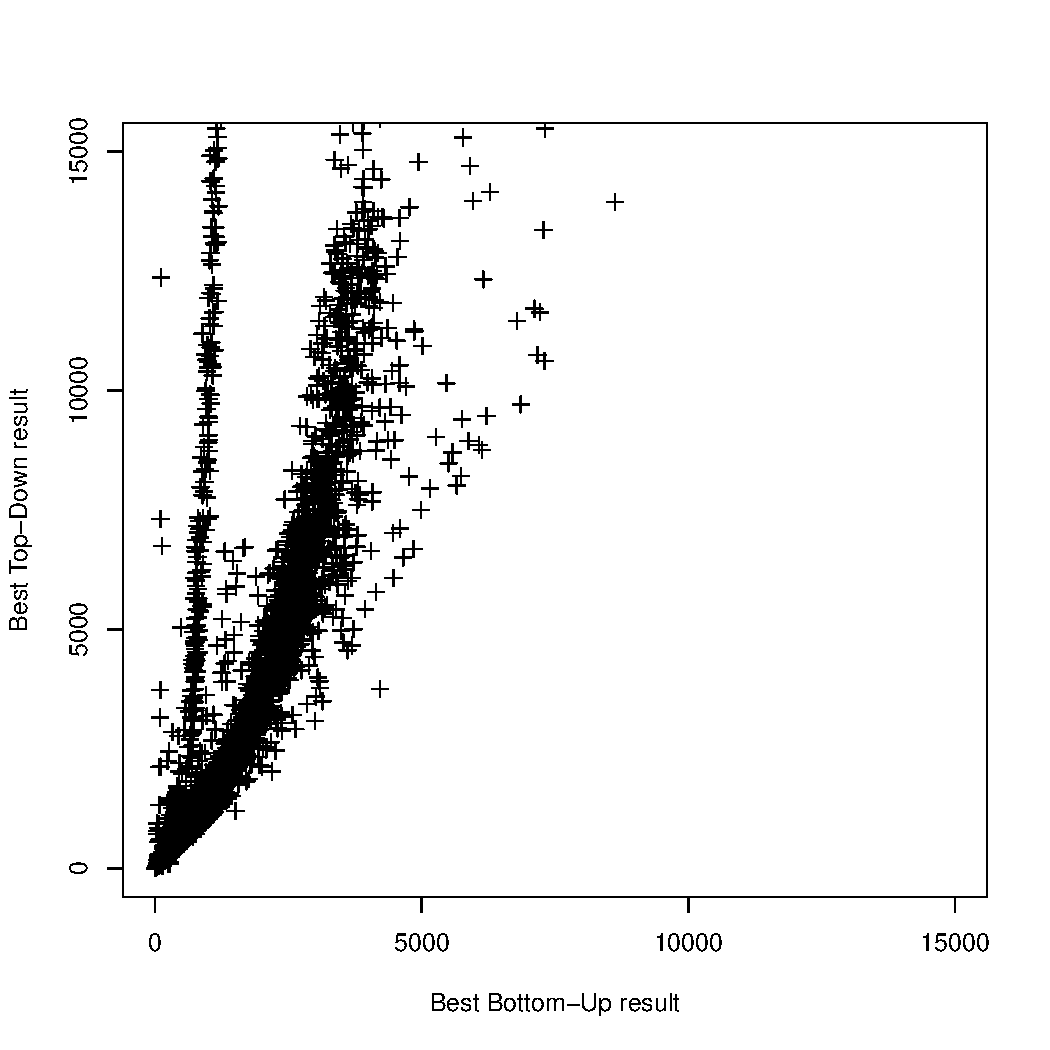
\includegraphics[scale=0.5]{chapters/pebbling/figures/td_vs_bu.pdf}
	\caption{Space measures of best Bottom-Up and Top-Down result}
	\label{fig:BUvsTD}
\end{figure}

The Bottom-Up algorithm does not only produce better results, it is also much faster, as can be seen in the last column of Table \ref{tab:results}. 
The reason probably is the number of comparisons that the algorithms make. 
For Bottom-Up the set $N$ of possible choices consists of the premises of a single node only, i.e. $|N| \in \{0,2\}$.
For Top-Down the set $N$ is the set of currently pebbleable nodes, which can be large (e.g. for a perfect binary tree with $2n -1$ nodes, initially $|N| = n$). 
Possibly for some heuristics, Top-Down algorithms could be made more efficient by using, instead of a set, an ordered sequence of pebbleable nodes together with their memorized heuristic evaluations.

Unsurprisingly the radius used for the Distance Heuristic has a severe impact on the speed, which decreases rapidly as the maximum radius increases. 
With radius 5, only a few small proofs were processed in a reasonable amount of time.

On average the smallest space measure of a proof is 44.1 times smaller than its length. 
This shows the impact that the usage of deletion information together with well constructed topological orders can have. 
When these techniques are used, on average 44.1 times less memory is required for storing nodes in memory during proof processing.


%%%%%%%%%%%%%%%%%%%%%%%%%%%%%%%%%%%%%%%%%
%%% Conclusion %%%%%%%%%%%%%%%%%%%%%%%%%%
%%%%%%%%%%%%%%%%%%%%%%%%%%%%%%%%%%%%%%%%%
%\chapter{Conclusion}
%\label{ch:conclusion}
%%%%%%%%%%%%%%%%%%%%%%%%%%%%%%%%%%%%%%%%%

Several algorithms for compressing proofs with respect to space have been conceived. The experimental evaluation clearly shows that the so-called Bottom-Up algorithms are faster and compress more than the more natural, straightforward and simple Top-Down algorithms. Both kinds of algorithms are parameterized by a heuristic function for selecting nodes. The best performances are achieved with the simplest heuristics (i.e. Last Child and Number of Children). More sophisticated heuristics provided little extra compression but cost a high price in execution time. Future work could investigate heuristics that take advantage of the particular shape of proofs generated by analysis of conflict graphs.

\vspace{-5pt}
\paragraph{Acknowledgments:} We would like to thank Armin Biere for clarifying why resolution chains are not left-associative in the TraceCheck proof format.

\vspace{-5pt}




%%%%%%%%%%%%%%%%%%%%%%%%%%%%%%%%%%%%%%%%%
%\chapter{Congruence}
%\label{ch:congruence}
%%%%%%%%%%%%%%%%%%%%%%%%%%%%%%%%%%%%%%%%%

\chapter*{Congruence}
\label{cha:congruence}
%\section{Congruence Closure}
\label{sec:congruencedef}

In this section we define the concepts of congruence- relation and closure, which is the foundation of our proof compression method.
To this end we define terms and equations, which are notions that will be used throughout this chapter.
We close this section by proving some elementary properties of congruence relations.

\begin{definition}[Terms and Subterms]

Let $\mathcal{F}$ be a finite set of function symbols and $arity: \mathcal{F} \rightarrow \mathbb{N}$.
A tuple $\Sigma = \langle \mathcal{F}, arity \rangle$ is a \emph{signature}.
A function symbol with arity zero is a \emph{constant}, one with arity one is a \emph{unary} function symbol and one with arity two is \emph{binary}.
For a given signature $\Sigma$, the set of \emph{terms} $\mathcal{T}^{\Sigma}$ is defined inductively.

\begin{align*}
	\mathcal{T}^{\Sigma}_0 &= \{a \in \mathcal{F} \mid arity(a) = 0\}\\
	\mathcal{T}^{\Sigma}_{i+1} &= \{g(t_1,\ldots,t_n) \mid arity(g) = n \text{ and } t_1, \ldots, t_n \in \mathcal{T}_{i}\} \\
	\mathcal{T}^{\Sigma} &= \bigcup_{i\in \mathbb{N}} \mathcal{T}^{\Sigma}_{i}
\end{align*}

\noindent Let $g(t_1,\ldots,t_n) \in \mathcal{T}^{\Sigma}$, then $t_1,\ldots,t_n$ are \emph{direct subterms} of $g(t_1,\ldots,t_n)$.
The \emph{subterm} relation is the reflexive, transitive closure of the direct subterm relation.
A term of the form $g(t_1,\ldots,t_n)$ is a \emph{compound term}.

\end{definition}

\noindent Should $\Sigma$ be clear from context or of no relevance, we will omit it and write $\mathcal{T}$ instead of $\mathcal{T}^{\Sigma}$.

\begin{definition}[Equation]

Let $\mathcal{T}$ be a set of terms.
An \emph{equation} of $\mathcal{T}$ is a tuple of terms, i.e. an element of $\mathcal{T} \times \mathcal{T}$.

\end{definition}

\noindent For a set of equations $E$ we denote by $\mathcal{T}_E$ the set of terms used in $E$.
$$\mathcal{T}_E := \{t \mid t \text{ is subterm of some } u \text{, such that for some } v: (u,v) \in E \text{ or } (v,u) \in E\}$$

\begin{definition}[Congruence Relation]

Let $\mathcal{T}$ be a set of terms.
A relation $R \subseteq \mathcal{T} \times \mathcal{T}$ is a congruence relation, if has the following four properties:
\begin{itemize}
	\item reflexivity: for all $t \in \mathcal{T}: (t,t) \in R$
	\item symmetry: $(s,t) \in R$ then $(t,s) \in R$
	\item transitivity: $(r,s) \in R$ and $(s,t) \in R$ then $(r,t) \in R$
	\item compatibility: $g$ is a n-ary function symbol and for all $i = 1,\ldots,n$ $(t_i,s_i) \in R$ then $(g(t_1,\ldots,t_n),g(s_1,\ldots,s_n)) \in R$
\end{itemize}

\end{definition}

Clearly every congruence relation is also an equivalence relation (which is a reflexive, transitive and symmetric relation).
Therefore every congruence relation partitions its underlying set of terms $\mathcal{T}$ into congruence classes, such that two terms $(s,t)$ belong to the same class if and only if $(s,t) \in R$.
The relations $\emptyset$ and $\mathcal{T} \times \mathcal{T}$ are trivial congruence relations.

In this work we are interested in congruence relations induced by sets of equations.
In other words, we compute the partitioning of the terms such that two terms in the same partition are proven to be equal by the input set of equations.
To this end we define the notion of congruence closure of a set of equations.

\begin{definition}[Congruence Closure]

Let $E$ be a set of equations.
The set $E^* \supseteq E$ is the \emph{congruence closure} of $E$, 
if $E^*$ is a congruence relation on $\mathcal{T}_E$ and for every congruence relation $C$, such that $C \supseteq E$ follows $C \supseteq E^*$.
We write $E \models s \thickapprox t$ if $(s,t) \in E^*$ and say that $E$ is an \emph{explanation} for $s \thickapprox t$.
We call a pair $(s,t)$ in a congruence closure an \emph{equality} and we call an equality of compound terms $(g(t_1,\ldots,t_n),g(s_1,\ldots,s_n))$ such that for all $i = 1,\ldots,n$: $E \models t_i \thickapprox s_i$ a \emph{deduced equality}.
For a term $t \in \mathcal{T}_E$ the set of congruent terms $\{s \in \mathcal{T}_E \mid E \models s \thickapprox t\}$ is the \emph{congruence class} of $t$.

\end{definition}

It is easily seen that congruence relations are closed under intersection.
Therefore $E^*$ always exists.

\begin{proposition}[Properties of the $\models$ relation]
\label{prop:models}
The $\models$ relation is monotone: $E_1 \subseteq E_2$ and $E_1 \models s \thickapprox t$ implies $E_2 \models s \thickapprox t$ and consistent: $E \models s \thickapprox t$ and $E \cup \{(s,t)\} \models u \thickapprox v$ implies $E \models u \thickapprox v$. 

\end{proposition}

\begin{proof}

Monotonicity follows from the fact that congruence closure of $E_1$ is contained in the congruence closure of $E_2$.

Since the congruence closure of $E^*$ is $E^*$ itself, it follows that $E \models u \thickapprox v$ if and only if $E^* \models u \thickapprox v$.
Since $(s,t) \in E^*$, clearly it is the case that $E^* = (E \cup \{(s,t)\})^*$.
Therefore $E \cup \{(s,t)\} \models u \thickapprox v$ implies $(u,v) \in E^*$, i.e. $E \models u \thickapprox v$ or in other words, the $\models$ relation is consistent.

\end{proof}


%\section*{Resolution extended with equality}

Let $\mathcal{T}$ be a set of terms.
A relation $R \subset \mathcal{T} \times \mathcal{T}$ is a congruence relation, if has the following four properties:
\begin{itemize}
	\item reflexive: for all $t \in \mathcal{T}: (t,t) \in R$
	\item symmetric: $(s,t) \in R$ implies $(t,s) \in R$
	\item transitive: $(r,s) \in R$ and $(s,t) \in R$ implies $(r,t) \in R$
	\item congruence: $f$ is a n-ary function symbol and for all $i = 1,\ldots,n (t_i,s_i) \in R$ implies $f(t_1,\ldots,t_n),f(s_1,\ldots,s_n) \in R$
\end{itemize}

Every congruence relation partitions its underlying termset $\mathcal{T}$ into congruence classes, s.t. two terms $(s,t)$ belong to the same class if and only if $(s,t) \in R$.
The relations $\mathcal{T} \times \mathcal{T}$ and $\emptyset$ are trivial congruence relations.

Let $E$ be a set of equations with terms in some set of terms $\mathcal{T}$.
The set $E* \supseteq E$ is called the congruence closure of $E$, 
if $E*$ is a congruence relation on $\mathcal{T}$ and for every congruence relation $C$, such that $C \supset E$ follows $C \supseteq E*$.
It is easily seen that congruence relations are closed under intersection.
Therefore $E*$ always exists.

We write $E \models s = t$ if $(s,t) \in E*$.

We now extend the resolution calculus, presented in Section \ref{TODO}, with the axioms of equality.


%\section{NP-completeness of Short Explanation Decision Problem}
\label{sec:npcomplete}
In Section \ref{sec:congruencedef} the notion of an explanation is defined and it was mentioned that we want to find short explanations in order to compress proofs.
In this section we show that one might have to search a while to find the shortest one, by proving that the problem of deciding whether there is an explanation of a given size is NP-complete.
Our proof of NP-completeness reduces the problem of deciding the satisfiability of a propositional logic formula  in conjunctive normal form (SAT) to the short explanation decision problem.
For basics about satisfiability of propositional logic formulas and assignments, we refer the reader to \cite{Biere2009}.
We begin by formally defining the problem.

\begin{definition}[Short explanation decision problem]

Let $E = \{(s_1,t_1),\ldots,(s_n,t_n)\}$ be a set of equations, $k \in \mathbb{N}$ and $(s,t)$ be a target equation.
The \emph{short explanation decision problem} is the question whether there exists a set $E'$ such that $E' \subseteq E$, $E' \models s \thickapprox t$ and $|E'| \leq k$.

\end{definition}

Our proof of hardness translates propositional formulas into sets of equations and proves properties of the resulting formulas.
To this end we define a general translation of formulas in conjunctive normal form into sets of equations.

\begin{definition}[Congruence Translation]

Let $\Phi$ be a propositional logic formula in conjunctive normal form with clauses $C_1,\ldots,C_n$ using variables $x_1,\ldots,x_m$.
%The set of terms $\mathcal{T}$ is constructed using the following constants and function symbols.
%For every $i= 1,\ldots,n + 1$, there is a constant $\hat{c}_i$ and function symbols $t_i$ and $f_i$.
%For every $j= 1,\ldots,m$, there are constants $\hat{x}_j$, $\top_j$ and $\bot_j$.
The congruence translation $E_{\Phi}$ of $\Phi$ is defined as the set of equations $Assignment \cup Pos \cup Neg \cup Connect$, where
\begin{align*}
	Assignment &= \{ (\hat{x}_j,\top_j), (\hat{x}_j,\bot_j) \mid 1 \leq j \leq m\} \\
	Pos &= \{ (\hat{c}_i, t_i(\hat{x}_j)) \mid x_j \text{ appears positively in } C_i\} \\
	Neg &= \{ (\hat{c}_i, f_i(\hat{x}_j)) \mid x_j \text{ appears negatively in } C_i\} \\
	Connect &= \{ (t_i(\top_j),\hat{c}_{i+1}),(f_i(\bot_j), \hat{c}_{i+1}) \mid 1 \leq i \leq n, 1 \leq j \leq m\} \\
%\end{align*}
&\hspace{-2cm}\text{For presentation purposes we define the following sets for every $i = 1,\ldots, n$ and $j = 1,\ldots, m$}\\
%\begin{align*}
T_{ij} &= \{(\hat{c}_i, t_i(\hat{x}_j)), (\hat{x}_j,\top_j), (t_i(\top_j),\hat{c}_{i+1})\} \\
F_{ij} &= \{(\hat{c}_i, f_i(\hat{x}_j)), (\hat{x}_j,\bot_j), (f_i(\bot_j),\hat{c}_{i+1})\}
\end{align*}

\end{definition}

The following examples shows the congruence translation of a propositional formula and a subset of the translation corresponding to a satisfying assignment.
We use the standard notion of satisfiability and present variable assignments as sets of those propositional variables being mapped to true.

\begin{example}

Let $\Phi := (x_1 \vee x_2 \vee \neg x_3) \wedge (\neg x_2 \vee x_3) \wedge (\neg x_1 \vee \neg x_2)$. 
Figures \ref{fig:npexamplebig}, \ref{fig:npassignment} and \ref{fig:npexplanation} present sets of equations graphically, where an edge between two nodes means that the respective set contains an equation between the two nodes.
Figure \ref{fig:npexamplebig} shows the graphical representation of the equations in $Pos, Neg$ and $Connect$ for the congruence translation $E_{\Phi}$ of $\Phi$.
Let $\mathcal{I} := \{x_1,x_3\}$. 
It is easy to see that $\mathcal{I} \models \Phi$.
Figure \ref{fig:npexplanation} shows a graphical representation of $\mathcal{I}$ in terms of equations.
This set of equations is an explanation for $(\hat{c}_1,\hat{c}_4)$.
Note that $\mathcal{I}' := \{x_1\}$ is another satisfying assignment and for the satisfiability of $\Phi$, the truth value of variable $x_3$ is not essential.
Therefore replacing $\{(\hat{x}_3,\top_3)\}$ by $\{(\hat{x}_2,\top_2)\}$ in the explanation corresponding to $\mathcal{I}$ leads to another explanation of $(\hat{c}_1,\hat{c}_4)$ of equal size.
However, this set does not represent an assignment, since it is not clear which truth value $x_2$ has.
In the proof of Lemma \ref{lemma:nphardness} we exclude such ambiguous sets by introducing additional topological clauses.
\begin{figure}[!h]


\centering
\begin{tikzpicture}[node distance=.3cm]

\node(c1){$\hat{c}_1$};

\node[right =.4cm of c1] (t1x2) {$t_1(\hat{x}_2)$};
\node[above =1cm of t1x2] (t1x1) {$t_1(\hat{x}_1)$};
\node[below =1cm of t1x2] (f1x3) {$f_1(\hat{x}_3)$};

\draw [-] (c1) to (t1x2);
\draw [-] (c1) to (t1x1);
\draw [-] (c1) to (f1x3);


\node[right =.4cm of t1x1, yshift = 0.25cm] (f11) {$f_1(\bot_1)$};
\node[above =.4cm of f11] (t11) {$t_1(\top_1)$};
\node[below =.4cm of f11] (t12) {$t_1(\top_2)$};
\node[below =.4cm of t12] (f12) {$f_1(\bot_2)$};
\node[below =.4cm of f12] (t13) {$t_1(\top_3)$};
\node[below =.4cm of t13] (f13) {$f_1(\bot_3)$};

\node[right = 4cm of c1](c2){$\hat{c}_2$};

\draw [-] (c2) to (t11);
\draw [-] (c2) to (t12);
\draw [-] (c2) to (t13);
\draw [-] (c2) to (f11);
\draw [-] (c2) to (f12);
\draw [-] (c2) to (f13);

\node[right =.25cm of c2, yshift=1cm]  (f2x2) {$f_2(\hat{x}_2)$};
\node[below =1.5cm of f2x2] (t2x3) {$t_2(\hat{x}_3)$};

\draw [-] (c2) to (f2x2);
\draw [-] (c2) to (t2x3);

\node[right =3cm of f11] (f21) {$f_2(\bot_1)$};
\node[right =3cm of t11] (t21) {$t_2(\top_1)$};
\node[right =3cm of t12] (t22) {$t_2(\top_2)$};
\node[right =3cm of f12] (f22) {$f_2(\bot_2)$};
\node[right =3cm of t13] (t23) {$t_2(\top_3)$};
\node[right =3cm of f13] (f23) {$f_2(\bot_3)$};

\node[right = 4cm of c2](c3){$\hat{c}_3$};

\draw [-] (c3) to (t21);
\draw [-] (c3) to (t22);
\draw [-] (c3) to (t23);
\draw [-] (c3) to (f21);
\draw [-] (c3) to (f22);
\draw [-] (c3) to (f23);

\node[right =.25cm of c3, yshift=1cm] (f3x1) {$f_3(\hat{x}_1)$};
\node[below =1.5cm of f3x1] (f3x2) {$f_3(\hat{x}_2)$};

\draw [-] (c3) to (f3x1);
\draw [-] (c3) to (f3x2);

\node[right =3.4cm of f21] (f31) {$f_3(\bot_1)$};
\node[right =3.4cm of t21] (t31) {$t_3(\top_1)$};
\node[right =3.4cm of t22] (t32) {$t_3(\top_2)$};
\node[right =3.4cm of f22] (f32) {$f_3(\bot_2)$};
\node[right =3.4cm of t23] (t33) {$t_3(\top_3)$};
\node[right =3.4cm of f23] (f33) {$f_3(\bot_3)$};

\node[right = 4.5cm of c3](c4){$\hat{c}_4$};

\draw [-] (c4) to (t31);
\draw [-] (c4) to (t32);
\draw [-] (c4) to (t33);
\draw [-] (c4) to (f31);
\draw [-] (c4) to (f32);
\draw [-] (c4) to (f33);

\end{tikzpicture}


\caption{Pos, Neg and Connect for $E_{\Phi}$}
\label{fig:npexamplebig}
\end{figure}


\begin{figure}[!h]


\centering
\begin{tikzpicture}[node distance=.75cm]

\node (x1) {$\hat{x}_1$};
\node [below =.5cm of x1] (x2) {$\hat{x}_2$};
\node [below =.5cm of x2] (x3) {$\hat{x}_3$};

\node [right = of x1] (t1) {$\top_1$};
\node [left = of x1] (f1) {$\bot_1$};

\draw [-] (x1) to (t1);
\draw [-] (x1) to (f1);

\node [right = of x2] (t2) {$\top_2$};
\node [left = of x2] (f2) {$\bot_2$};

\draw [-] (x2) to (t2);
\draw [-] (x2) to (f2);

\node [right = of x3] (t3) {$\top_3$};
\node [left = of x3] (f3) {$\bot_3$};

\draw [-] (x3) to (t3);
\draw [-] (x3) to (f3);

\end{tikzpicture}



\caption{Assignment for $E_{\Phi}$}
\label{fig:npassignment}
\end{figure}

\begin{figure}[!h]


\centering
\begin{tikzpicture}
\tikzstyle{every node}=[font=\small]
\node(c1){$\hat{c}_1$};

\node[right =.2cm of c1] (t1x1) {$t_1(\hat{x}_1)$};

\draw [-] (c1) to (t1x1);

\node[right =.1cm of t1x1] (t11) {$t_1(\top_1)$};

%\draw [dashed] (t1x1) to (t11);

\node[right =.2cm of t11](c2){$\hat{c}_2$};

\draw [-] (c2) to (t11);

\node[right =.2cm of c2]  (f2x2) {$f_2(\hat{x}_2)$};

\draw [-] (c2) to (f2x2);

\node[right =.1cm of f2x2] (f22) {$f_2(\bot_2)$};

%\draw [dashed] (f2x2) to (f22);

\node[right = .2cm of f22](c3){$\hat{c}_3$};

\draw [-] (c3) to (f22);

\node[right =.2cm of c3] (f3x2) {$f_3(\hat{x}_2)$};

\draw [-] (c3) to (f3x2);

\node[right =.1cm of f3x2] (f32) {$f_3(\bot_2)$};

%\draw [dashed] (f3x2) to (f32);

\node[right =.2cm of f32](c4){$\hat{c}_4$};

\draw [-] (c4) to (f32);

\node [below =.5cm of t1x1] (x1) {$\hat{x}_1$};

\node [right =.5cm of x1] (t1) {$\top_1$};

\node [right =1cm of t1] (f2) {$\bot_2$};


\node [right =.5cm of f2] (x2) {$\hat{x}_2$};

\node [right =1cm of x2] (x3) {$\hat{x}_3$};


\node [right =1cm of x3] (t3) {$\top_3$};

\draw [-] (x1) to (t1);

\draw [-] (x2) to (f2);


\draw [-] (x3) to (t3);

\end{tikzpicture}


\caption{Explanation of $(\hat{c}_1,\hat{c}_4)$}
\label{fig:npexplanation}
\end{figure}

\end{example}


\begin{lemma}[Characterization of explanations]
\label{lemma:charexpl}

Let $\Phi$ be a propositional logic formula in conjunctive normal form with $n$ clauses and $m$ variables.
For every subset $E$ of $E_{\Phi}$, $E \models \hat{c}_1 \thickapprox \hat{c}_{n+1}$ if and only if for every $i = 1,\ldots,n$ there is a $j = 1,\ldots,m$ such that $T_{ij} \subseteq E$ or $F_{ij} \subseteq E$.

\end{lemma}

\begin{proof}

Suppose that for every $i = 1,\ldots,n$ there is a $j = 1,\ldots,m$ such that $T_{ij} \subseteq E$ or $F_{ij} \subseteq E$.
Clearly $T_{ij} \models \hat{c}_i \thickapprox t_i(\hat{x}_j)$ and $T_{ij} \models t_i(\top_j) \thickapprox \hat{c}_{i+1}$. 
Since $(\hat{x}_j,\top_j) \in E$, the fact $E \models t_i(\hat{x}_j) \thickapprox t_i(\top_j)$ follows by an application of the monotonicity axiom.
Using the transitivity of congruence relations, it follows that $T_{ij} \models \hat{c}_i \thickapprox \hat{c}_{i+1}$.
Similarly it can be shown that $F_{ij} \models \hat{c}_i \thickapprox \hat{c}_{i+1}$.
Therefore it follows from the assumption that $E \models \hat{c}_i \thickapprox \hat{c}_{i+1}$ for every $i = 1,\ldots,n$.
Using the transitivity again, it follows that $E \models \hat{c}_1 \thickapprox \hat{c}_{n+1}$.

\noindent We show the other implication of the equivalence by induction on $n$.
\begin{paragraph}{Induction Base $n = 1$:}

Suppose that $E \models \hat{c}_1 \thickapprox \hat{c}_{2}$. %, which implies $\hat{c}_2 \in [\hat{c}_1]_E$.
Since $\hat{c}_1$ is a constant, the compatibility of congruence relations can not be applied to extend the congruence class of $\hat{c}_1$ beyond the singleton $\{\hat{c}_1\}$.
Therefore in order to satisfy $E \models \hat{c}_1 \thickapprox u$ with $u \neq \hat{c}_1$ there has to be an equation $(\hat{c}_1, u) \in E$ for some term $u$.
Since $E \subseteq E_{\Phi}$, the only possible such equations are $(\hat{c}_1, t_1(\hat{x}_j))$ and $(\hat{c}_1, f_1(\hat{x}_j))$ for some $j$.
The only equations in $E$ involving terms with the function symbols $t_1$ and $f_1$ are $(\hat{c}_1, t_1(\hat{x}_j)), (t_1(\top_j),\hat{c}_2)$ and $(\hat{c}_1, f_1(\hat{x}_j)), (f_1(\bot_j),\hat{c}_2)$ for some $j$.
Therefore in order to satisfy $E \models \hat{c}_1 \thickapprox u$ such that $u$ is neither the constant $\hat{c}_1$, nor some term $t_1(\hat{x}_j), f_1(\hat{x}_j)$, it is necessary that $E \models t_1(\hat{x}_j) \thickapprox t_1(\top_j)$ and $(\hat{c}_1, t_1(\hat{x}_j)) \in E$ or $E \models f_1(\hat{x}_j) \thickapprox f_1(\bot_j)$ and $(f_1(\bot_j),\hat{c}_2) \in E$ for some $j$.
The conditions can only be satisfied with equations of $E_{\Phi}$ if $\{(\hat{c}_1, t_1(\hat{x}_j)), (\hat{x}_j,\top_j)\} \subseteq E$ or $\{(\hat{c}_1, f_1(\hat{x}_j), (\hat{x}_j,\bot_j)\} \subseteq E$ respectively.
%Similarly $t \in [\hat{c}_1]_E$ such that $t$ is neither $\hat{c}_1$ nor a term with the function symbol $t_1$ or $f_1$, for some $j$ $(t_1(\top_j),\hat{c}_2) \in E$ and 
From a similar argumentation about the equations involving $\hat{c_2}$ and $t_1(\top_j)$ or $f_1(\bot_j)$ it follows that either $T_{1j} \subseteq E$ or $F_{1j} \subseteq E$ for some $j$.
\end{paragraph}

\begin{paragraph}{Induction Hypothesis:} For every subset $E$ of $E_{\Phi}$, $E \models \hat{c}_1 \thickapprox \hat{c}_{n}$ if and only if for every $i = 1,\ldots,n-1$ there is a $j = 1,\ldots,m$ such that $T_{ij} \subseteq E$ or $F_{ij} \subseteq E$.
\end{paragraph}

\begin{paragraph}{Induction Step:}
Suppose that $E \models \hat{c}_1 \thickapprox \hat{c}_{n+1}$.\\
Similarly to the argumentation in the induction base, the only equations in $E_{\Phi}$ involving $\hat{c}_{n+1}$ are of the form $(t_n(\top_j),\hat{c}_{n+1})$ and $(f_n(\bot_j),\hat{c}_{n+1})$.
The only possibility to enrich the congruence class of $\hat{c}_{n+1}$ with terms other than $\hat{c}_{n+1}$ and those of the form $t_n(\top_j)$ and $f_n(\bot_j)$, 
is that for some $j$, $(\hat{x}_j,\top_j) \in E$ or $(\hat{x}_j,\bot_j) \in E$ and subsequently also $(\hat{c}_n,t_n(\hat{x}_j)) \in E$ or $(\hat{c}_n,f_n(\hat{x}_j)) \in E$.
Thus $T_{nj} \subseteq E$ or $F_{nj} \subseteq E$ and as a consequence $E \models \hat{c}_n \thickapprox \hat{c}_{n+1}$.
Using transitivity $E \models \hat{c}_1 \thickapprox \hat{c}_{n+1}$ and $E \models \hat{c}_n \thickapprox \hat{c}_{n+1}$ imply $E \models \hat{c}_1 \thickapprox \hat{c}_n$ and from the induction hypothesis it follows that  $T_{ij} \subseteq E$ or $F_{ij} \subseteq E$ for every $i = 1,\ldots,n-1$.
\end{paragraph}

\end{proof}

\begin{lemma}[NP- hardness]
\label{lemma:nphardness}
The short explanation decision problem is NP- hard.

\end{lemma}

\begin{proof}

We reduce SAT to the short explanation decision problem.
SAT is a well known NP-complete problem \cite{Biere2009}.
Let $\Phi$ be a propositional formula in conjunctive normal form with clauses $C_1,\ldots,C_n$ and variables $x_1,\ldots,x_m$.
Let $C_{n+1},\ldots,C_{n+m}$ be the tautological clauses $\{x_1, \neg x_1\},\ldots,\{x_m,\neg x_m\}$.
Clearly $\Phi$ is satisfiable if and only if $\Phi' = \{C_1,\ldots,C_{n+m}\}$ is satisfiable.
We will show that $\Phi'$ is satisfiable if and only if there exists $E \subseteq E_{\Phi'}$ such that $E \models \hat{c}_1 \thickapprox \hat{c}_{n+m+1}$ and $|E| \leq 2n + 3m$.

\emph{Suppose} $\Phi'$ is satisfiable and let $\mathcal{I}$ be a satisfying assignment.\\
For every clause $C_i$ there is a literal $\ell_i \in C_i$, such that $\mathcal{I} \models \ell_i$.
For every $i = 1,\ldots,n+m$ we set $E_i:= T_{ij}$ if $\ell_i = x_j$ and $E_i:= F_{ij}$ if $\ell_i = \neg x_j$.
From $\ell_i \in C_i$ follows $E_i \subseteq E_{\Phi'}$.
Let $E = \bigcup_i^n E_i$ then from Lemma \ref{lemma:charexpl} and the transitivity of the congruence relations follows $E \models c_1 \thickapprox c_{n+m+1}$.
What remains to show is that $|E| \leq 2n + 3m$.
Since the sets $Pos, Neg$ and $Connect$ in the definition of $E_{\Phi'}$ are pairwise disjoint, for $i \neq j$ $E_i \cap E_j \subseteq \{(\hat{x}_j,\top_j),(\hat{x}_j,\bot_j) \mid j = 1,\ldots,m\}$.
Therefore $E$ involves exactly $2(n+m)$ equations of $Pos, Neg$ and $Connect$.
By construction of the sets $E_i$ and the clauses $C_{n+1},\ldots,C_{n+m}$ there is no $j = 1,\ldots,m$ such that $(\hat{x}_j,\top_j) \in E$ and $(\hat{x}_j,\bot_j) \in E$.
Therefore $E$ involves $m$ equations of set $Assignment$ in the definition of $E_{\Phi'}$.
Overall we have $|E| = 2n + 3m$.

\emph{Suppose} there exists $E \subseteq E_{\Phi'}$, $E \models \hat{c}_1 \thickapprox \hat{c}_{n+m+1}$ and $|E| \leq 2n + 3m$.\\
We will show that $\mathcal{I} = \{\hat{x}_j \mid (\hat{x}_j,\top_j) \in E\}$ is a satisfying assignment for $\Phi'$.
Let $i = 1,\ldots,n+m$ be an arbitrary clause index.
From $E \models \hat{c}_1 \thickapprox \hat{c}_{n+m+1}$ and Lemma \ref{lemma:charexpl} follows $T_{ij} \subseteq E$ or $F_{ij} \subseteq E$ for some $j=1,\ldots,m$.
Assume $T_{ij} \subseteq E$ for some $j = 1,\ldots,m$.
$E \subseteq E_{\Phi'}$ implies that $x_j$ appears positively in $C_i$. 
By definition of $\mathcal{I}$, $\mathcal{I} \models x_j$ and therefore $\mathcal{I} \models C_i$.
If $T_{ij} \nsubseteq E$ for all $j = 1,\ldots,m$, then $F_{ij} \subseteq E \subseteq E_{\Phi'}$, which implies that $x_j$ appears negatively in $C_i$, $x_j \notin \mathcal{I}$ and therefore $\mathcal{I} \models C_i$. Since $i$ was arbitrary we conclude $\mathcal{I} \models \Phi'$.

\end{proof}

\begin{lemma}[In NP]
\label{lemma:innp}
The short explanation decision problem is in NP.

\end{lemma}
\begin{proof}

Explanations are subsets of the input equations, therefore they are clearly polynomial in the problem size.
The congruence of two terms, i.e. verifying that a subset is actually an explanation, can be decided in $O(n \log(n))$ using for example the congruence closure algorithm presented in Section \ref{sec:algorithms}.

\end{proof}

Lemma \ref{lemma:nphardness} and \ref{lemma:innp} establish the main result of this section.

\begin{theorem}[NP - completeness]

The short explanation decision problem is NP- complete.

\end{theorem}

\section{Explanation Producing Congruence Closure}
\label{sec:algorithm}
%
In this section we present a congruence closure algorithm that is able to produce explanations.
The algorithm is a mix of the approaches of the algorithms presented in \cite{Fontaine2004} and \cite{Nieuwenhuis2005,Nieuwenhuis2007}.
The basic structure of the algorithm is inherited from \cite{Fontaine2004}, which itself inherits its structure from the algorithm of Nelson and Oppen \cite{Nelson1980}.
The technique to store and deduce equalities of non constant terms is inspired by \cite{Nieuwenhuis2005,Nieuwenhuis2007}.
Additionally the proof forest structure described below was proposed by \cite{Nieuwenhuis2005,Nieuwenhuis2007}.

Before we describe the algorithm, we discuss two technical concepts that are important aspects of our congruence closure algorithm.

\subsection*{Currification and Abstract Congruence Closure}
\label{subsec:algorithms_preliminaries}

Our congruence closure algorithm operates on curried terms.
Curried terms use a single binary function symbol to represent general terms.
More formally, let $\mathcal{F}$ be a finite set of functions with a designated binary function symbol $f \in \mathcal{F}$ and let every other function symbol in $\mathcal{F}$ be a constant.
A term w.r.t. a signature of this form is called a \emph{curried term}.

It is possible to uniquely translate a general set of terms $\mathcal{T}^{\Sigma}$ with signature $\Sigma = \langle \mathcal{F},arity \rangle$ into a set of curried terms $\mathcal{T'}^{\Sigma'}$.
The new signature $\Sigma'$ is obtained from $\Sigma$ by setting $arity$ to zero for every function symbol in $\mathcal{F}$ and introducing the designated binary function symbol $f$ to $\mathcal{F}$.
The translation of a term $t \in \mathcal{T}^{\Sigma}$ is given in terms of the function $curry$.

$$
curry(t) = \Big\{
\begin{array}{ll}
	t & \text{ if } t \text{ is a constant }\\
	f(\ldots (f(f(g,curry(t_1)),curry(t_2)))\ldots,curry(t_n)) &\text{ if } t = g(t_1,\ldots, t_n)
\end{array}
$$

The idea of currying was introduced by M. Sch\"onfinkel \cite{Schoenfinkel1924} in 1924 and independently by Haskell B. Curry \cite{Curry1958} in 1958, who also lends his name to the concept.
Currying is not restricted to terms.
The general idea is to translate functions of type $A \times B \rightarrow C$ into functions of type $A \rightarrow B \rightarrow C$.
There is a close relation between currying and lambda calculus \cite{Church1936}.
Lambda calculus uses a single binary function $\lambda$.
Its arguments can either be elements of some set or again lambda terms.
For an introduction to lambda calculus, including currying in terms of lambda calculus and its relation to functional programming, see \cite{Barendregt1997}.

The benefit of working with curried terms is an easier and cleaner congruence closure algorithm, while maintaining best known runtime for congruence closure algorithms of $O(n \log(n))$.
Curried terms simplify the algorithm, because case distinctions on terms are much simpler.
A curried term is either a constant or a compound term of the form $f(a,b)$, where $a$ and $b$ are curried terms.
To deal with all kinds of general terms, different leading function symbols and their arities have to be taken into account.
Cleaner algorithms are not only easier to implement, but should also improve the practical runtime for similar reasons.

Recently so called abstract congruence closure algorithms have been proposed and shown to be more efficient than traditional approaches \cite{Bachmair2000}.
The idea of abstract congruence closure is to introduce new constants for non constant terms.
Doing so, all equations the algorithm has to take into account are of the form $(c,d)$ and $(c, f(a,b))$, where $a,b,c,d$ are constants.
This replaces tedious preprocessing steps, for example transformation to a graph of outdegree 2 \cite{Downey1980},that are necessary for other algorithms to achieve the optimal running time.

Our method is does not employ the idea of abstract congruence closure.
We found that using currying is enough to obtain an algorithm with optimal running time and no tedious preprocessing steps.
The reason why we did not go for abstract congruence closure is, that we do not want to have the overhead of introducing and eliminating fresh constants.
In the context of proof compression, our congruence closure algorithm will be applied to relatively small instances very often.
We could introduce the extra constants for the whole proof before processing, but would still have to remove them from explanations every time we produce a new subproof.
It would be interesting to investigate, whether our intuition in that regard is right, or if it pays off to deal with extra constants.

\cite{Nieuwenhuis2005,Nieuwenhuis2007} describes an explanation producing abstract congruenc closure algorithm, 
whereas \cite{Fontaine2004} proposes a traditional algorithm without currying and extra constants.
By choosing to work with curried terms, but without extra constants, our algorithm is a middle ground between the two algorithms.

\subsection*{Immutable Data Structures}

Most of the data structures presented the following section are defined in terms of mathematical functions.
This is not by coincidence and our congruence closure algorithm can easily be translated to an implementation in a functional programming language.
Furthermore, all data structures can be implemented immutable.
An immutable data structure is one that never changes is internal state after its creation.
When alternating the information stored in the data structure, a new object with the new information is constructed.
The old object remains intact.
A side effect of a method is a modification of an object that is not the returned value of the method.
Such side effects often lead to bugs, since the method can not be used as a black box anymore.
An example for a side effect is the modification of the representative of a term in the congruence closure algorithm presented in \cite{Fontaine2004} and its effect on what is called signature table in this work.
Using immutable data structures prohibits side effects by design.
Furthermore immutable data structures allow to maintain internal correctness much easier.
For example, in the Skeptik tool resolution nodes are stored in an immutable fashion.
Modifying the premise of a node does not have an effect on the node itself, since its premise remains to be the old version.
Therefore the correctness of a resolution proof, once established when creating a proof is maintained without any further actions.
Functional programming languages almost exclusively use immutable data structures and often it is not easy or impossible to translate an imperative description of an algorithm into functional programming.
Sometimes it is possible, but not with the same runtime.

Immutable data structures also have some downsides.
The impossibility of changing internal structures often makes it hard to maintain certain structures without a lot of extra effort.
One simple example is that of a linked list.
Suppose such a linked list is implemented in such a way that every element of the list internally has a pointer to the next element in the list.
When modifying the first element of the list in some fashion, the pointer of the second element has to be set to the new version of the first one.
Since this requires to produce a new version of the second element as well, also the pointer of the third element has to be updated and so on.
Some algorithms and their optimal runtime depend on such data structures, that are very hard or impossible to implement immutable.
However, sometimes tricky data structures like the zipper were invented which help to overcome these problems.

\subsection*{Congruence structure}

We call the underlying data structure of our congruence closure algorithm a \emph{congruence structure}.
A congruence structure for set of terms $\mathcal{T}$ is a collection of the following data structures.
The set $\mathcal{E} = \mathcal{T} \times \mathcal{T} \cup \{\smiley\}$ is the set of \emph{extended equations}.
The symbol $\smiley$ serves as a placeholder for deduced equalities that have to be explained in terms of input equations.

\begin{itemize}
	\item Representative $r: \mathcal{T} \rightarrow \mathcal{T}$
	\item Congruence class $[.]: \mathcal{T} \rightarrow 2^\mathcal{T}$
	\item Left neighbors $N_l: \mathcal{T} \rightarrow 2^\mathcal{T}$
	\item Right neighbors $N_r: \mathcal{T} \rightarrow 2^\mathcal{T}$
	\item Lookup table $l: \mathcal{T} \times \mathcal{T} \rightarrow \mathcal{T}$
	\item Congruence graph $g$
	\item Queue $\mathcal{Q}$ of pairs of terms
	\item Current explanations $\mathcal{M}: \mathcal{T} \times \mathcal{T} \rightarrow \mathcal{E}$
\end{itemize}

The representative is one particular term of a class of congruent terms.
It is used to identify whether two terms are in the same congruence class and the data structures ($l, N_l$ and $N_r$) used for detecting deduced equalities are kept updated only for representatives.
The congruence class structure represents a set of pairwise congruent terms.
It is used to keep track which representatives have to be updated when merging the classes of two terms.
The structures left $N_l$ (resp. right $N_r$) neighbor  keeps track of the respective other terms in compound terms.
The information is only used for representatives (i.e. terms in the target of $r(.)$).
Furthermore right and left neighbors always only contain one term per congruence class (which is not necessarily the representative of that class).
The lookup table is used to keep track of all compound terms in the congruence structure and to merge classes of compound terms, which arguments are congruent.
For example if the terms $f(a,b),f(c,d)$ were inserted and the representatives are such that $r(a) = r(c), r(b) = r(d)$, then $N_r(r(a)) = \{d\}$, $N_l(r(d)) = \{a\}$ and $l(r(a),r(b)) = f(a,b)$.
The elements in the respective sets serve as pointers to their representatives, therefore it does not matter whether for example $N_r(r(a)) = \{d\}$ or $N_r(r(a)) = \{b\}$.
In Section \ref{sec:congruenceclosurealgorithm} we explain how these structures are modified and used in detail.
The congruence graph (explained in detail in Section \ref{sec:congruencegraph}) stores the derived equalities in a structured way, that allows to create explanations for a given pair of terms.
Edges are added to the graph in a lazy way, meaning that they are buffered and only actually entered into the graph when demanded.
The queue $\mathcal{Q}$ keeps track of the order in which edges should be added to the graph.
The function $\mathcal{M}$ stores explanations if they exist for buffered edges.
The idea will be explained in detail in Section \ref{sec:proofproduction}.
We call the unique congruence structure for $\mathcal{T} = \emptyset$ the \emph{empty congruence structure}.

\FloatBarrier

\subsection*{Congruence closure algorithm}
\label{sec:congruenceclosurealgorithm}
In this section we present our explanation producing congruence closure algorithm and state and prove its properties.
Most importantly we show that the algorithm is sound and complete and has the best known asymptotic running time $O(n \log(n))$, where $n$ is the number of terms in the input.
Computing the congruence closure of some set of equations $E$ is done by adding all equations to an ever growing congruence structure, which initially is empty.
Since this has to be done in some order, we will often assume that $E$ is given as a sequence of equations rather than a set.
The pseudocode of most methods do not include return statements.
In fact every method implicitly returns a (modified) congruence structure or simply modifies a global variable, which is the current congruence structure.
Adding an equation to a congruence structure is done with the \texttt{addEquation} method, which is the only method that has to be visible to the user.
The method adds boths sides of the equation to the current set of terms using the \texttt{addNode} method and afterwards merges the classes of the two terms.
The \texttt{addNode} method enlarges the set of terms and detects deduced equalities.
The updates of the set of terms are not outlined explicitly, but are understood to happen implicitly.
Throughout this chapter we denote this implicit set of terms by $\mathcal{T}$.
The method \texttt{merge} initializes and guides the merging of congruence classes.
The actual merging is done by the method \texttt{union} by modifying the data structures.
The method does not only merge classes, but also searches for and returns deduced equalities.
The classes of the terms of these extra equalities are merged, if they are not equal yet.
The congruence classes are kept track of in a graph, maintaining important information for producing explanation and proofs.
We call such a graph Congruence Graph and explain them in a more detailed fashion in Section \ref{sec:congruencegraph}.
Edges, that reflect detected equalities, are not inserted into the graph right away, but stored in queue until the insertion is requested.
The reason for adding edges in a lazy way is to produce shorter explanations and proofs and will be explained and exemplified in Section \ref{sec:proofproduction}.

\begin{algorithm}[t]
\caption[.]{addEquation}
  \KwIn{equation $s=t$ or null}
	
	addNode($s$) \\
	addNode($t$) \\
	merge($s, t, s=t$)
  
  \label{algo:addEquation}
\end{algorithm}


\begin{algorithm}[t]
	\caption[.]{addNode}
  \KwIn{term $v$}
	
	\If{$r$ is not defined for $v$}
		{$r(v) \leftarrow v$ \\
		$[v] \leftarrow \{v\}$ \label{initclass} \\
		$N_l(v) \leftarrow \emptyset$ \\
		$N_r(v) \leftarrow \emptyset$ \label{initrN} \\
		\If{$v$ is of the form $f(a,b)$}{
			addNode(a) \\
			addNode(b) \\
			\eIf{$l$ is defined for $(r(a),r(b))$ and $l(r(a),r(b)) \neq f(a,b)$ \label{ldefined}}{
				merge($l(r(a),r(b)),f(a,b),\smiley$) \label{addnodemerge} 
			}
			{
				$l(r(a),r(b)) \leftarrow f(a,b)$ \label{initl} 
			}
			$N_l(r(b)) \leftarrow N_l(r(b)) \cup \{a\}$ \\
			$N_r(r(a)) \leftarrow N_r(r(a)) \cup \{b\}$ \label{modifyrN}\\
			%\KwAssert{Neighbours \nllabel{invariant:neig_add}} 
		 }
	}
	
  
  \label{algo:addNode}
\end{algorithm}


\begin{algorithm}[t]
\caption[.]{merge}
  \KwIn{term $s$}
	\KwIn{term $t$}
	\KwIn{extended equation $eq$}
	
	\If{$r(s) \neq r(t)$}{
		$c \leftarrow \{s=t\}$ \\
		$eq \leftarrow s=t$ \\
		\While{$c \neq \emptyset$}{
			Let $(u,v)$ be some element in $c$ \\
			$c \leftarrow c \setminus \{(u,v)\} \cup union(u,v)$ \\
			lazy\_insert$(u,v,eq)$ \\
			$eq \leftarrow null$
		}
	}
  \KwAssert{$r(s) = r(t)$ \nllabel{assertion:merge_rep}}
  \label{algo:merge}
\end{algorithm}


\begin{algorithm}[t]
\caption[.]{union}
  \KwIn{term $s$}
	\KwIn{term $t$}
	\KwOut{a set of deduced equations}
	
	\eIf{$[r(s)] \geq [r(t)]$}{
		$(u,v) \leftarrow (s,t)$
	}
	{
		$(u,v) \leftarrow (t,s)$
	}
	$d \leftarrow \emptyset$ \\
	\nllabel{startlN}\For{every $x \in lN(r(v))$}{
		$l_v \leftarrow l(r(x),r(v))$ \\
		\eIf{$r(x) = r(v)$}{
			$new_left \leftarrow r(u)$
		}{
			$new_left \leftarrow r(x)$
		}
		\eIf{$l$ is defined for $(new\_left,r(u))$}{
			$l_u \leftarrow l(new\_left,r(u))$ \\
			\eIf{$r(l_u) \neq r(l_v)$}{
				\nllabel{deduceEq1} $d \leftarrow d \cup \{(l_u,l_v)\}$
			}
			{
				$lN(r(v)) \leftarrow lN(r(v)) \setminus \{x\}$
			}
		}
		{
			\nllabel{changel2} $l(new\_left,r(u)) \leftarrow l_v$
		}
	\nllabel{stoplN}}
	\nllabel{startrN}\For{every $x \in rN(r(v))$}{
		$l_v \leftarrow l(r(v),r(x))$ \\
		\eIf{$r(x) = r(v)$}{
			$new_right \leftarrow r(u)$
		}{
			$new_right \leftarrow r(x)$
		}
		\eIf{$l$ is defined for $(r(u),new\_right)$}{
			$l_u \leftarrow l(r(u),new\_right)$ \\
			\eIf{$r(l_u) \neq r(l_v)$}{
				\nllabel{deduceEq2} $d \leftarrow d \cup \{(l_u,l_v)\}$
			}
			{
				$rN(r(v)) \leftarrow rN(r(v)) \setminus \{x\}$
			}
		}
		{
			\nllabel{changel1} $l(r(u),new\_right) \leftarrow l_v$
		}
	\nllabel{stoprN}}
	\nllabel{changeclass} $[r(u)] \leftarrow [r(u)] \cup [r(v)]$ \\
	\For{every $x \in [r(v)]$}{
		\nllabel{changerep} $r(x) \leftarrow r(u)$
	}
	\nllabel{changeclass} $[r(u)] \leftarrow [r(u)] \cup [r(v)]$ \\
	$lN(r(u)) \leftarrow lN(r(u)) \cup lN(r(v))$ \\
	\nllabel{modifyrN2} $rN(r(u)) \leftarrow rN(r(u)) \cup rN(r(v))$ \\
	\KwInvariant{Neighbours \nllabel{invariant:neig_union}} \\
	\KwAssert{$r(s) = r(t)$ \nllabel{assertion:union_rep}}
	\Return $d$
  \label{algo:union}
\end{algorithm}



\begin{algorithm}[h]
\caption[.]{lazy\_insert}
  \KwIn{term $s$}
	\KwIn{term $t$}
	\KwIn{extended equation $eq$}
	%\KwGlobal{Queue of tuples of terms $\mathcal{Q}$}
	%\KwGlobal{Map of tuples of terms to equation $\mathcal{M}$}
	
	\eIf{$\mathcal{M}$ is set for $(s,t)$ or $(t,s)$}{
		\If{eq is not null}{
			$\mathcal{M}(s,t) \leftarrow s = t$ 
		}
	}{
		$\mathcal{Q} \leftarrow \mathcal{Q}.enqueue(s,t)$ \\
		$\mathcal{M}(s,t) \leftarrow eq$ 
	}
  
  \label{algo:lazyinsert}
\end{algorithm}


\begin{algorithm}[h]
\caption[.]{lazy\_update}
	%\KwIn{congruence graph $g$}
	%\KwGlobal{Queue of tuples of terms $\mathcal{Q}$}
	%\KwGlobal{Map of tuples of terms to equation $\mathcal{M}$}
	
	\While{$\mathcal{Q}$ is not empty}{
		$(u,v) \leftarrow \mathcal{Q}.dequeue$\\
		$eq \leftarrow \mathcal{M}(u,v)$ \\
		$g.insert(u,v,eq)$
	}
  
  \label{algo:lazyupdate}
\end{algorithm}



In the following pages, we will provide some invariants that are essential for proving the properties of the algorithm.
The invariants hold when initializing the respective data structures and before and after every insertion of an equation via the \texttt{addEquation} method.

\begin{invariant}[Class]

For every $s \in \mathcal{T}$ and every $t \in [r(s)]$, $r(t) = r(s)$.

\label{invar:class}
\end{invariant}
%{\color{blue} For all invariants I might need to be more specific as to when exactly they should old.}
\begin{proof}

Clearly the invariant is true when intializing $[s]$ in line \ref{initclass} of \texttt{addNode}.

The only other point in the code that changes $[s]$ is line \ref{changeclass} of union.
Suppose the class of $u$ is enlarged by the class of $v$ in union and suppose the invariant holds before the union for those terms.
Before the update of $[r(u)]$ the representative of every term in $[r(v)]$ is set to $r(u)$.
Therefore the invariant remains valid after the update.

\end{proof}

\begin{invariant}[Lookup]

The lookup structure $l$ is defined for a pair of terms $(s,t)$ if and only if there is a term $f(a,b) \in \mathcal{T}$ such that $r(a) = r(s)$ and $r(b) = r(t)$.

\end{invariant}

\begin{proof}

Suppose $l$ is defined for some pair of terms $(s,t)$.
The value of $l(s,t)$ is set either in lines \ref{changel1} or \ref{changel2} of \texttt{union} or in line \ref{line:initl} of \texttt{addNode}.
In the latter case, $l$ is set to $f(a,b)$ for the tuple $(r(a),r(b))$ and therefore the invariant holds at this point.
For changes to $r(a)$ or $r(b)$ in union the one implication of the invariant remains valid in case $l$ is defined for the new representatives, or $l$ is set for an additional pair of terms in lines \ref{changel1} or \ref{changel2}.
In case $l$ is set to $(new\_left,r(u))$ or $(r(u),new\_right)$ in union, there is an $l$-entry $l_v$ for which the invariant held before the union.
The changes in representatives of $x$ are reflected by $new\_left$ and $new\_right$, while the representative of $v$ is changed to $r(u)$.
The new entry for $l$ therefore respects the implication of the invariant.

To show the other implication, let $f(a,b) \in \mathcal{T}$.
The term $f(a,b)$ is entered with the \texttt{addEquation} method and subsequently via the \texttt{addNode} method.
For compound terms lines \ref{line:ldefined} and \ref{line:initl} assert that $l$ is defined for $(r(a),r(b))$.
All changes to $r(a)$ or $r(b)$ must happen in \texttt{union} and they are reflected by matching updates to the $l$ structure.

\end{proof}


\begin{invariant}[Neighbours]

For every $s \in \mathcal{T}$, every $t_r \in N_r(r(s))$ and $t_l \in N_l(r(s))$, $l$ is defined for $(r(s),r(t_r))$ and $(r(t_l),r(s))$.

\end{invariant}

\begin{proof}

We show the result for the structure $N_r$.
The result about $N_l$ can be obtained analogously.
Since $N_r$ is initialized with the empty set in line \ref{initrN} of \texttt{addNode}, the invariant clearly holds initially.
To show that the invariant always holds, it has to be shown that all modifications of $r$ and $N_r$ preserve the invariant.
The structure $l$ is not modified after initialization.
Line \ref{modifyrN} of \texttt{addNode} adds $b$ to $N_r(r(a))$ and the four lines before that addition show that $l$ is defined for $(r(a),r(b))$.
Union modifies $N_r$ in such a way that it adds all right neighbors of some representative $r(v)$ to $N_r(r(u))$.
Lines \ref{startrN} to \ref{stoprN} make sure that $l$ is defined for all these right neighbors.
Updates of $r$ in \ref{changerep} are always followed by corresponding updates to $N_r$.

\end{proof}

A consequence of this invariant is the fact that, that for every term $t \in \mathcal{T}$ of the form $f(a,b)$, $l$ is defined for $(r(a),r(b))$.

\begin{proposition}[Sound- \& Completeness]

Let $r(.)$ be the representative mapping obtained by adding equations $E = \langle (u_1,v_1), \ldots, (u_n,v_n) \rangle $ to the empty congruence structure.
For every $s,t \in \mathcal{T}_E$: $E \models s \thickapprox t$ if and only if $r(s) = r(t)$.

\end{proposition}

\begin{proof}
\textbf{Completeness}

\noindent We show that from $E \models s \thickapprox t$ follows $r(s) = r(t)$ by induction on $n$.

\begin{itemize}
\item \textbf{Induction Base} $n=1$: $E \models s \thickapprox t$ implies either $s = t$ or $\{u_1,v_1\} = \{s,t\}$.
In the first case $r(s) = r(t)$ is trivial. 
In the second case, the claim follows from the fact that, when $(u_1,v_1)$ is entered, union is called with arguments $s$ and $t$.
After this operation $r(s) = r(t)$.

\item \textbf{Induction Hypothesis}: For every sequence of equations $E_n$ with $n$ elements and every $s,t \in \mathcal{T}_{E_n}$: $E_n \models s \thickapprox t$ then $r(s) = r(t)$.

\item \textbf{Induction Step}: Let $E = \langle (u_1,v_1), \ldots, (u_{n+1},v_{n+1}) \rangle$ and $E_n = \langle (u_1,v_1), \ldots, (u_n,v_n) \rangle$.
There are two cases: $E_n \models s\thickapprox t$ and $E_n \nvDash s\thickapprox t$.
In the former case, the claim follows from the induction hypothesis, the invariant class and the fact that union always changes representatives for all elements of a class.
We still have to show the claim in the latter case.
We write $E \models_n u \thickapprox v$ as an abbreviation for $E_n \nvDash u \thickapprox v$ and $E \models u \thickapprox v$.
We show the claim ($E \models s \thickapprox t$) by induction on the structure of the terms $s$ and $t$.

\begin{itemize}
\item \textbf{Induction Base} $s$ or $t$ is a constant and therefore transitivity reasoning was used to derive $E \models_n s \thickapprox t$.
In other words, there are $l$ terms $t_1,\ldots,t_l$ such that $s = t_1$, $t = t_l$ and for all $i = 1,\ldots,l-1: E \models_n t_i \thickapprox t_{i+1}$.
We prove by yet another induction on $l$ that $r(t_1) = r(t_l)$.
\begin{itemize}
\item \textbf{Induction Base} $l = 2$. It has to be the case (up to swapping $u_{n+1}$ with $v_{n+1}$), that $E_n \models s \thickapprox u_{n+1}$ and $E_n \models t \thickapprox v_{n+1}$, and the outmost induction hypothesis implies $r(s) = r(u_{n+1})$ and $r(t) = r(v_{n+1})$.
Therefore it follows from Invariant Class, that after the call to union for $(u_{n+1},v_{n+1})$ it is the case that $r(t_1) = r(t_2)$.

\item \textbf{Induction Step}: suppose that the claim holds for all sequences of length $l \in \mathbb{N}$, for $l+1$ the claim follows from a simple application of the transitivity axiom, since $t_1,\ldots,t_l$ and $t_2,\ldots,t_{l+1}$ are both sequences of length $l$.
\end{itemize}
\item \textbf{Induction Step}: suppose that $s = f(a,b)$ and $t = f(c,d)$.
There are two cases such that $E \models_n s \thickapprox t$ can be derived.
Using a transitivity chain, the claim can be shown just like in the base case.
Using the compatability axiom, it has to be the case that $E \models_n a \thickapprox c$ and $E \models_n b \thickapprox d$ (in fact one of those can also be the case without the $n$ index).
The terms $a,b,c,d$ are of lower structure than $s$ and $t$.
Therefore it follows from the induction hypothesis that $r(a) = r(c)$ and $r(b) = r(d)$.
The Invariants Neighbour and Lookup imply that either $r(s) = r(t)$ or $(s,t)$ is added to $d$ in line \ref{deduceEq1} or line line \ref{deduceEq2} of union.
Subsequently union is called for $s$ and $t$, after which $r(s) = r(t)$ holds.
\end{itemize}
\end{itemize}

\noindent\textbf{Soundness}

\noindent For $s = t$ the claim follows trivially.
Therefore we show soundness in case $s \neq t$.
We show that from $r(s) = r(t)$ follows $E \models s \thickapprox t$ by induction on the number $m$ of calls to union induced by adding all equations of $E$ to the empty congruence structure, for all $s$ and $t$ that are arguments of some call to union.
The original claim then follows from invariant Class, since only union modifies the $r$ structure and the fact that two terms are in the same class if and only if union was called for some elements in the respective classes.
%Notice that only union modifies $r$ after initialization.
%Therefore the proof investigates the changes made by union and the parameters it is called when adding equations to a congruence structure.
\begin{itemize}
\item \textbf{Induction Base} $m = 1$: $r(s) = r(t)$ implies $\{u_1,v_1\} = \{s,t\}$ and $E \models s \thickapprox t$ is trivial.
%Lines \ref{deduceEq1} and \ref{deduceEq2} do not induce any further unions, because no compound terms, that $s$ or $t$ could be a subterm of, are yet inserted in the congruence structure.

%Induction hypothesis: For every sequence of equations $E_n$ with $n$ elements and every $s,t \in \mathcal{T}_{E_n}$: $r(s) = r(t)$ after adding all $n$ equations to the empty congruence structure then $E_n \models s \thickapprox t$.

\item \textbf{Induction Hypothesis}: For every $k < m$, if a set of equations $F$ induces $k$ calls to union, then from $r(s) = r(t)$ follows $F \models s \thickapprox t$ for all terms $s,t$ that are arguments of some call to union.

\item \textbf{Induction Step}: Suppose $E = \langle (u_1,v_1), \ldots, (u_n,v_n) \rangle$ induces $m$ calls to union with arguments $(h_1,g_1),\ldots,(h_m,g_m)$.
The subsequence $E_n = \langle (u_1,v_1), \ldots, (u_{n-1},v_{n-1}) \rangle$ induced the first $l$ calls to union for some $n-1 \leq k < m$.
In other words, adding $(u_n,v_n)$ to the congruence structure induces $m-k-1$ calls to union with arguments $(h_{k+1},g_{k+1}),\ldots,(h_m,g_m)$.
The pair $(h_{k+1},g_{k+1})$ is either an original input equation, or a deduced equality from line \ref{addnodemerge} of \texttt{addNode}.
In both cases $E \models h_{k+1} \thickapprox g_{k+1}$, which is trivial in the former case and an application of the induction hypothesis in the latter case.
Let $j \in \{k+2,\ldots,m\}$.
The pair $(h_j,g_j)$ was inserted to $d$ in line \ref{deduceEq1} or \ref{deduceEq2} of \texttt{union} that was called with arguments $(h_i,g_i)$ with $i \in \{k+1,\ldots,j-1\}$, such that subterm ...
Therefore, using induction on the structure of terms, the original induction hypothesis, Invariants Lookup and Neighbour and lines \ref{startlN} to \ref{stoprN} of \texttt{union}, it can be shown that for all pairs $(h_k,g_k)$ and all $k = l+1,\ldots,m$ it is the case that $E \models h_k \thickapprox g_k$.

%
%We show the induction step by another induction on $k-l$, i.e. the number of unions induced by adding $(u_n,v_n)$ to the congruence structure.
%Base case $k-l = 1$: Union is called for $(u_n,v_n)$ and the induces no further calls union.
%After the one call to union $r(u_n) = r(v_n)$ and clearly $E \models u_n \thickapprox v_n$.
%The fact that lines \ref{deduceEq1} and \ref{deduceEq2} of union do not induce any further calls to the method, together with the induction hypothesis and the invariants Lookup and Neighbour, imply that $E \models_n s \thickapprox t$ if and only if $s,t = \{u_n,v_n\}$.
%
%Induction step: Suppose adding $(u_n,v_n)$ induces $m$ calls to union with arguments $(h_{k-m},g_{k-m}),\ldots,(h_k,g_k)$.
%The last call to union has to be added 
%
%Adding the equation $(u_{n+1},v_{n+1})$ to the working congruence structure induces a sequence of $l$ calls to union with parameters $(h_1,g_1),\ldots,(h_l,g_l)$

%After initialization of $r$ only union modifies the structure.
%Adding $E$ to the empty congruence structure induces a sequence of calls to union with parameters $(u_1,v_1), \ldots , (u_n,v_n)$.
%We show by induction on $n$, that $E \models v_i \thickapprox u_i$
\end{itemize}
\end{proof}

\begin{proposition}[Runtime]
\label{prop:runtime}
Let $E$ be a set of equations such that $|\mathcal{T}_E| = n$.
Computing the congruence closure with our congruence closure algorithm takes worst-case time $O(n \log(n))$.

\end{proposition}

\begin{proof}

There are three loops in the method \texttt{union}, which are nested within the loop of \texttt{merge}.
These loops are clearly the dominating factor for runtime.
Lines \ref{reverse1} and \ref{reverse2} of \texttt{union} swap the arguments $s$ and $t$ in such a way, that always the congruence class of $v$ is smaller than the one of $u$.
Let $k$ be the size of the congruence class of $v$ before the union.
For every term in the congruence classes of $v$ and $u$ before the union, the size of their new congruence class after the union (set in line \ref{changeclass}) is at least $2*k$.
Furthermore, only representatives for terms in the old congruence class of $v$ are changed in line \ref{changerep}.
This implies that for every term, whenever its representative is changed in line \ref{changerep}, its congruence class doubles in the same execution of \texttt{union}.
The maximum size of a congruence class is $n$.
Therefore the representative of a single term is changed in line \ref{changerep} maximally $\log(n)$ times.
There are $n$ terms that can be changed, so line \ref{changerep} of \texttt{union} is executed at most $n \log(n)$ times.
Let $f(a,b)$ be the result of accessing $l$ in line \ref{accessl1}.
In the same call of \texttt{union} line \ref{changerep} changes the representative of $b$.
Since this this happens only $\log(n)$ times and there are at most $m < n$ compound terms, line \ref{accessl1} is executed at most $n \log(n)$ times.
The same holds for line \ref{accessl1} and all other lines in the respective loops.

\end{proof}


\FloatBarrier

\subsection*{Congruence Graph}
\label{sec:congruencegraph}
The most important feature of our congruence closure algorithm towards proof compression is explanation production.
For this purpose the input equations and deduced equalities have to be stored in a data structure that supports this feature.
We support two different such data structures.
Both structures store equalities in labeled graphs, which we call congruence graphs and have methods.
A node in such a graph represents a term and an edge between two nodes denotes that the represented terms are congruent w.r.t. the set of input equations.
A path in a congruence graph is a sequence of undirected, unweighted, labeled edges in the underlying graph.
The set of labels for both types of graphs is the set of extended equations $\mathcal{E}$ (i.e. equations and the placeholder \smiley).
The method \texttt{merge} adds edges to the graph via the \texttt{lazy\_insert} method, which eventually calls the \texttt{insert} method, which is different for the two structures.
After calling \texttt{insert} with arguments $s$ and $t$ it is guaranteed that there is a path in the congruence graph between $s$ and $t$.
In case they were not connected before the call, then there is an edge between $s$ and $t$ after the call.
The same can be assumed for \texttt{lazy\_insert} since edges that are added to the queue are never discarded and $s$ and $t$ are connected virtually.
The methods \texttt{insert} and \texttt{explain} are assumed to be attached to the data structures.
For example adding an edge to the data structure means adding it to the used congruence graph.

\begin{invariant}[Paths]

For terms $s, t$ such that $s \neq t$ holds $r(s) = r(t)$ if and only if there is a path in the congruence graph of the structure between $s$ and $t$

\end{invariant}

\begin{proof}

We show the claim by an induction on $|[r(s)]|$.
%We show that there is a path between $s$ and $t$ in the congruence graph induction on $|[r(s)]|$. 
The proof relies on the invariant Class, which shows the consistency between classes and representatives.

\begin{itemize}
\item \textbf{Induction Base:} $[r(s)] = \{s\}$, i.e. $r(s) = r(t)$ is false for every term $t \neq s$.
We have to show that there is no edge $(s,t)$ for $t \neq s$ in the congruence graph.
Edges are only added to the congruence graph via the \texttt{lazy\_insert} method which is only called in \texttt{merge}.
Clearly \texttt{merge} does not call \texttt{union} for $s$ and some term $t \neq s$, since otherwise $t \in [r(s)]$.
Therefore \texttt{merge} also does not add an edge for $s$ and some term $t \neq s$ to the congruence graph.

\item \textbf{Induction Hypethesis:} For every term $s$ such that $|[r(s)]| \leq n$ and for every term $t \neq s$ it is the case that $r(s) = r(t)$ if and only if there is a path between $s$ and $t$ in the congruence graph.

\item \textbf{Induction Step:} Suppose $[r(s)]$ is an arbitrary class with cardinality $n+1$.
Then there are two terms $u,v \in [r(s)]$ such that \texttt{union} was called for $u$ and $v$.
Before the union $|[r(u)]|$ and $|[r(v)]|$ both were strictly smaller than $n+1$.
In case they both belong to the same class before the union, the claim follows trivially by the induction hypothesis, since existing paths are not removed by adding new edges to the graph.
Suppose $s \in [r(u)]$ and $t \in [r(v)]$, then by induction hypothesis there are paths $p_1$ between $s$ and $u$ and $p_2$ between $t$ and $v$.
Right after the union of $u$ and $v$, an edge is inserted between them, so $p_1$ concatenated with $(u,v)$ and $p_2$ is a path between $s$ and $t$.
In case one of the terms did not belong to one of the classes before the union, it does not belong to the merged class after the union.
Also there was no path between the two terms before and since the only addition paths are between elements of $[r(u)]$ and $[r(v)]$, there is no path between the terms after the union.
\end{itemize}

\end{proof}

\begin{invariant}[Deduced Edges]

For every edge in a congruence structure between vertices $u,v$ with label $\smiley$, 
there are $a,b,c,d \in \mathcal{T}$ such that $u = f(a,b)$, $v = f(c,d)$ and
there are paths in the underlying graphs between $a$ and $c$ as well as between $b$ and $d$.

\end{invariant}

\begin{proof}

Edges with label $\smiley$ are added, when \texttt{merge} is called from \texttt{addNode}, or \texttt{union} induces an additional merge.
In both cases there are subterms with respective congruent representatives.
The claim follows by using the invariant Paths.

\end{proof}

The method \texttt{explain} returns a path between its two arguments, if one exists.
There can be more than one such path depending on the actual type of graph used.
The method \texttt{inputEqs} for a path in the congruence graph returns the input equations that were used to derive the equality between the first and the last node of the path.
For an input equation, this is simply the equation itself.
For a deduced equality, this is the set of input equations that were used for deduction.
Combining these two methods, the statement \texttt{inputEqs(explain(s,t,g),g)} for input equations $E$ returns an explanation $E' \subseteq E$ such that $E' \models s \thickapprox t$ if there is one.

\begin{algorithm}[h]
\caption[.]{inputEqs}
	\KwIn{path $p$}
	\KwOut{set of input equations used in $p$}
	
	Let $p$ be $(u_1,l_1,v_1),\ldots,(u_n,l_n,v_n)$\\
	$eqs \leftarrow \emptyset$ \\
	\For{$i \leftarrow 1 \text{ to }n$}{
		\eIf{$l_i = \smiley$}{
			$f(a,b) \leftarrow u_i$ \\
			$f(c,d) \leftarrow v_i$ \\
			$p1 \leftarrow $ explain$(a,c)$ \\
			$p2 \leftarrow $ explain$(b,d)$ \\
			$eqs \leftarrow eqs \cup inputEqs(p1) \cup inputEqs(p2)$
		}{
			$eqs \leftarrow eqs \cup \{l_i\}$
		}
	}
	\Return{$eqs$}
  
  \label{algo:inputeqs}
\end{algorithm}


In the following, we describe the two types of congruence graphs we support.
They differ in the underlying type of graph, how edges are inserted and how explanations are produced.

\subsubsection*{Equation Graph}

An equation graph stores equalities in an edge labeled weighted undirected graph $(V,E)$ with 
$V \subseteq \mathcal{T}$, $E \subseteq V \times \mathcal{E} \times V \times \mathbb{N}$.
The weight for an edge is the number of input equations used to derive the equality between its two nodes.
This number is one for input equalities and the size of the explanation for deduced equalities.
Edges are added to the graph, regardless whether the nodes are already connected in the graph.
Therefore there is a choice which path the explain method returns.
We look for short explanations and the weights reflect sizes of sub explanation.
Therefore we want to return the shortest path.

Finding the shortest path between two nodes in a weighted graph is not trivial.
The single source shortest path problem (SSSP) is a classical graph problem in computer science.
The task is to find the shortest path in a graph between one designated node, the source, and all other nodes in the graph.
To the best knowledge of the authors, there is no algorithm to find the shortest path between two nodes which has better asymptotic runtime than one to solve SSSP.
There is a whole variety of algorithms that solve SSSP.
Classical algorithms for SSSP are those of Dijkstra \cite{Dijkstra1959} and Bellman-Ford \cite{Ford1956,Bellman1956}.
The algorithms work on different kinds of graphs.
Our setting is an undirected graph with positive integer weights.
We chose to use Dijkstra's algorithm, even though the algorithm does not have optimal asymptotic runtime.
Its worst-case runtime is $O(n \log(n))$ \cite{Cormen1989}, if the priority queue is implemented as a Fibonacci Heap, which is the case in our implementation.
\cite{Thorup1999} reports of an linear time algorithm for the undirected single source shortest path with positive integer weights problem.
However, the algorithm has a big overhead and needs several precomputations.
\cite{Cherkassky1996} presents a comparative study of several shortest path algorithms which shows that Dijkstra's algorithm performs well in practice.

Dijkstra's algorithm finds shortest paths to an increasing set of nodes, until every node has been discovered.
It does so by keeping track of the the shortest paths and the distances, being the combined weights of edges on the path, of nodes to the source.
Initially, the only discovered node is the source itself and the distance to every other node is infinite.
The algorithm discovers new nodes by selecting the lowest weight outgoing edge of all nodes that have been discovered so far and updates shortest paths and distances while doing so.
It is a greedy algorithm in the sense that it always locally chooses lowest weight edges and never discards previously made decisions.

The algorithm has been slightly modified to take into account decisions that are edges for deduced equalities.
These edges represent explanations, which are sets of input equations.
In the same call to the search algorithm, using such equations again to explain another equality does not increase the size of the overall explanation.
The modified Dijkstra algorithm temporarily adds an edge with weight 0 for every input equation in the explanation of a deduced equality edge.
This is done to possibly reduce the size of explanations.
Since previous decisions are not discarded, it is not guaranteed that the modified algorithm returns the shortest path in the final graph, including the extra edges.
Example \ref{ex:short_expl} demonstrates that the modified shortest path algorithm does not always produce the shortest explanation, but can produce shorter explanations than the unmodified version in some situations.
The shortest path algorithm's inability to return shortest explanations is not surprising, since it runs in $O(n \log(n))$ and in Section \ref{sec:npcomplete} it is shown that finding the shortest explanation is NP-complete.

\begin{example}
Consider the congruence graph shown in Figure \ref{fig:short_expl}, where solid edges are input equation and the dashed edge marks an application of the congruence axiom.
The equality of $f(c_1,e)$ and $f(c_4,e)$ was deduced using the equations $(c_1,c_2),(c_2,c_3),(c_3,c_4)$, which is the shortest path in the graph between $c_1$ and $c_4$, obtained from a previous call to the shortest path algorithm.

Suppose we want to compute an explanation for $a \thickapprox b$.
Clearly the input equalities $(a,f(c_1,e))$, $(f(c_4,e),c_1)$ and the explanation for $f(c_1,e) \thickapprox f(c_4,e)$ have to be included in the explanation.
Additionally $c_1 \thickapprox b$ has to be explained.
For this equality the set $(c_1,d_1),(d_1,d_2),(d_2,b)$ is the shortest explanation in the original graph.
This sub explanation adds three new equations to the explanation for $a \thickapprox b$.
When the modified Dijkstra algorithm iterates over the edge $(f(c_1,e),f(c_4,e))$, it can add add zero weight edges $(c_1,c_2),(c_2,c_3),(c_3,c_4)$ to the graph.
By doing so the shortest explanation for $c_1 \thickapprox b$ becomes $(c_1,c_2),(c_2,c_3),(c_3,c_4),(c_4,b)$, which only adds one extra equation $(c_4,b)$ to the global explanation.
The resulting explanation contains six input equations.

This method is successful in finding the shortest explanation in this example if the search begins in the node $a$.
Should the search begin in the node $b$, the edges including $d_1$, $d_2$ are added to the shortest path before the edge $(f(c_1,e),f(c_4,e))$ is touched.
Therefore the undesired long explanation, including eight input equations, is returned.

\begin{figure}[!h]

\centering
\begin{tikzpicture}[node distance=1.5cm]

\node(a){$a$};

\node(f1)[right = .5cm of a]{$f(c_1,e)$};

\node(f2)[right = .5cm of f1]{$f(c_4,e)$};

\node(c1)[right = .5cm of f2]{$c_1$};

\node(c2)[right = .5cm of c1]{$c_2$};

\node(c3)[right = .5cm of c2]{$c_3$};

\node(c4)[right = .5cm of c3]{$c_4$};

\node(b)[right = .5cm of c4]{$b$};

\node(d1)[above = .25cm of c2]{$d_1$};

\node(d2)[above = .25cm of c4]{$d_2$};

\draw (a) -- (f1)  node [midway, above, sloped] {\small{1}};

\draw (f1) -- (f2) [-,dashed] node [midway, above, sloped] {\small{3}};

\draw (f2) -- (c1) node [midway, above, sloped] {\small{1}};

\draw (c1) -- (c2) node [midway, above, sloped] {\small{1}};

\draw (c2) -- (c3) node [midway, above, sloped] {\small{1}};

\draw (c3) -- (c4) node [midway, above, sloped] {\small{1}};

\draw (c4) -- (b) node [midway, above, sloped] {\small{1}};

\draw (c1) -- (d1) node [midway, above, sloped] {\small{1}};

\draw (d1) -- (d2) node [midway, above, sloped] {\small{1}};
  
\draw (d2) -- (b) node (test) [midway, above, sloped] {\small{1}};

\end{tikzpicture}

\caption{Short explanation example}
\label{fig:short_expl}
\end{figure}

\label{ex:short_expl}
\end{example}

\begin{algorithm}[h]
\caption[.]{insert (equation graph)}
  \KwIn{term $s$}
	\KwIn{term $t$}
	\KwIn{extended equality $eq \in \mathcal{E}$}
	%\KwIn{equation graph $g$}
	
	\eIf{$eq \neq \smiley$}{
		add edge $(s,eq,t,1)$ to $g$
	}
	{
		$f(a,b) \leftarrow s$ \\
		$f(c,d) \leftarrow t$ \\
		$p1 \leftarrow $ shortest path between $a$ and $c$ in $g$ \\
		$p2 \leftarrow $ shortest path between $b$ and $d$ in $g$ \\
		$w \leftarrow \#(p1.inputEqs \cup p2.inputEqs) $ \\
		add edge $(s,\smiley,t,w)$ % to $g$
	}
  
  \label{algo:insert_dij}
\end{algorithm}


\begin{algorithm}[h]
\caption[.]{explain}
  \KwIn{term $s$}
	\KwIn{term $t$}
	\KwIn{equation graph $g$}
	\KwOut{Path in $g$}
	
	\Return shortest path between $s$ and $t$ in $g$
	
  \label{algo:explain_dij}
\end{algorithm}



\FloatBarrier

\subsubsection*{Proof Forest}

A proof forest is a collection of proof trees.
A proof tree is a labeled tree with nodes in $\mathcal{T}$ and edge labels in $\mathcal{E}$.
For every congruence class in the current status of a congruence structure, there is one proof tree.
Inserting an edge between nodes $s$ and $t$ of different proof trees is done by making one the child of the other.
To maintain a tree structure, all edges between the new child and the root of its tree are reversed.
To limit the number of edge revering steps, the smaller tree is always attached to the bigger one.
This results in $O(n \log(n))$ edge reversing steps, where $n$ is the number terms in the input equation set.
This bound can be shown using the same argument as in the proof of Proposition \ref{prop:runtime}.
As stated above, we understand a path as a sequence of undirected edges.
In case of a proof tree, a path between $s$ and $t$ of the same tree is the combined sequence of edges between the nodes and their nearest common ancestors.
The structure, up to small changes, was proposed by \cite{Nieuwenhuis2005,Nieuwenhuis2007}.
Its benefit is the quick access of explanations and good overall runtime.
Its downside is its inflexibility when it comes to producing alternative explanations.
In fact the explanation returned is always the first one to occur during edge insertion.
The authors of \cite{Nieuwenhuis2005,Nieuwenhuis2007} improve the structure for the special case of flattened terms, for which no term has nesting depth greater than one.

\begin{algorithm}[h]
\caption[.]{insert (proof forest)}
  \KwIn{term $s$}
	\KwIn{term $t$}
	\KwIn{equation $eq \in \mathcal{E}$}
	%\KwIn{proof forest $g$}
	
	\If{$s$ is not in $g$}{
		add tree with single node $s$ %to $g$
	}
	\If{$t$ is not in $g$}{
		add tree with single node $t$ %to $g$
	}
	
	$sSize \leftarrow $ size of tree of $s$ \\ %in $g$ \\
	$tSize \leftarrow $ size of tree of $t$ %in $g$
	
	\eIf{$sSize \leq tSize$}{
		$(u,v) \leftarrow (s,t)$
	}{
		$(u,v) \leftarrow (t,s)$
	}

	reverse all edges on the path between $u$ and its root node \\
	insert edge $(v,eq,u)$% into $g$

  \label{algo:insert_pt}
\end{algorithm}


\begin{algorithm}[h]
\caption[.]{explain}
  \KwIn{term $s$}
	\KwIn{term $t$}
	%\KwIn{proof forest $g$}
	
	\eIf{$s$ and $t$ are in the same proof tree $P$}{
		Let $nca$ be the nearest common ancestor of $s$ and $t$ in $P$\\
		$p1 \leftarrow $ path from $s$ to $nca$ \\
		$p2 \leftarrow $ path from $nca$ to $s$ \\
		\Return $p1 :: p2$
	}{
		\Return the empty path
	}

  \label{algo:explain_pt}
\end{algorithm}




\begin{example}

Consider again the set of equations presented in Figure \ref{fig:short_expl} and Example \ref{ex:short_expl} and suppose that the equations $(c_1,d_1),(d_1,d_2),(d_2,b)$ are inserted into the congruence structure before any other equation.
After adding these three equations, the proof forest contains of a single proof tree and is displayed in Figure \ref{fig:proof_forest_1}, where the labels are omitted.
Suppose that next following equations are inserted: $(a,f(c_1,e)),(f(c_4,e),c_1),(c_1,c_2),(c_2,c_3)$.
The resulting proof forest contains two proof trees and is shown in Figure \ref{fig:proof_forest_2}.
Finally the equation $(c_3,c_4)$ is added and the equality $f(c_1,e) \thickapprox f(c_4,e)$ is deduced.
At this point, the explanation for $c_1 \thickapprox c_4$ in the proof forest is the path $\langle c_1,c_2,c_3,c_4 \rangle$, which is the combined path from $c_1$ and $c_4$ to their nearest common ancestor, which is $c_2$.
The resulting proof forest is shown in Figure \ref{fig:proof_forest_3}, where the explanation for the edge $(f(c_1,e),f(c_4,e))$ is highlighted in a dotted rectangle.
The explanation for $a \thickapprox b$ in this graph is the path $\langle b,d_2,d_1,c_1,f(c_4,e),f(c_1,e),a\rangle$ and since the edge $(f(c_1,e),f(c_4,e))$ uses all other equations as explanation, the final explanation includes all eight equations.
In example \ref{ex:short_expl} we have shown that this is not necessary.

\begin{figure}[!h]

\centering
\begin{tikzpicture}[node distance=1cm]



\node(d1){$d_1$};

\node(c1)[below left=of d1]{$c_1$};

\node(d2)[below right= of d1]{$d_2$};

\node(b)[below= of d2]{$b$};

\draw [->] (c1) -- (d1);% node [midway, above, sloped] {\small{1}};

\draw [->] (d2) -- (d1);% node [midway, above, sloped] {\small{1}};
  
\draw [->] (b) -- (d2);% node (test) [midway, above, sloped] {\small{1}};

\end{tikzpicture}

\caption{Proof Forest including first three equations}
\label{fig:proof_forest_1}
\end{figure}

\begin{figure}[!h]

\centering
\begin{tikzpicture}[node distance=1cm]

\node(c2){$c_2$};

\node(c3)[below left=of c2]{$c_3$};

\node(c1)[below right=of c2]{$c_1$};

\node(t1)[below left=of c1]{$f(c_4,e)$};

\node(d1)[below right=of c1]{$d_1$};

\node(d2)[below= of d1]{$d_2$};

\node(b)[below= of d2]{$b$};

\node(t2)[right =of c2,xshift=2cm]{$f(c_1,e)$};

\node(a)[below =of t2]{$a$};

\draw [->] (c3) -- (c2);
\draw [->] (d1) -- (c1);
\draw [->] (c1) -- (c2);
\draw [->] (d2) -- (d1);
\draw [->] (b) -- (d2);
\draw [->] (t1) -- (c1);

\draw [->] (a) -- (t2);

\end{tikzpicture}

\caption{Proof Forest before deducing}
\label{fig:proof_forest_2}
\end{figure}

\begin{figure}[!h]

\centering
\begin{tikzpicture}[node distance=1cm]
\node(t1){$f(c_4,e)$};

\node(c1)[below =of t1]{$c_1$};

\node(c2)[below of=c1]{$c_2$};

\node(c3)[below =of c2]{$c_3$};

\node(c4)[below =of c3]{$c_4$};

\node(d1)[below right=of c1]{$d_1$};

\node(d2)[below= of d1]{$d_2$};

\node(b)[below= of d2]{$b$};

\node(t2)[below left=of t1]{$f(c_1,e)$};

\node(a)[below =of t2]{$a$};

\node[rectangle,rounded corners,draw,dotted,fit=(c1) (c2) (c3) (c4)](rect) {};

\draw [->] (c4) -- (c3);
\draw [->] (c3) -- (c2);
\draw [->] (d1) -- (c1);
\draw [->] (c2) -- (c1);
\draw [->] (d2) -- (d1);
\draw [->] (b) -- (d2);
\draw [->] (c1) -- (t1);
\draw [->] (t2) -- (t1) node [midway, below] (expl) {};
\draw [->] (a) -- (t2);
\draw [->,dotted] (expl) -- (rect);

\end{tikzpicture}

\caption{Final Proof Forest}
\label{fig:proof_forest_3}
\end{figure}

\end{example}

%See how BarceLogic ppl prove stuff,
%-) tree is still tree after inserting
%-) path to NCA forms explanation


\FloatBarrier

%\section{Proof Production}
\label{sec:proofproduction}

In this section we describe how to produce resolution proofs from paths in a congruence graph.
The method to carry out this operation is \texttt{prodcureProof}.
The basic idea is to traverse the path, creating a transitivity chain of equalities between adjacent nodes, while keeping track of the deduced equalities in the chain.
From invariant Deduced Edges follows that for the deduced equalities there have to be paths between the respective arguments of the compound terms.
These paths are transformed into proof recursively and resolved with a suiting instance of the congruence axiom.
Afterwards the subproof is resolved with the original transitivity chain.
Since terms can never be equal to their (non trivial) subterms, the procedure will eventually terminate.
The result of this procedure is a resolution proof with a root, such that the equations of the negative literals are an explanation of the target equality or $\emptyset$ to denote that the equality can not be proven.
Suppose some equality $s \thickapprox t$ can be explained and \texttt{produceProof} returns a proof with root $\rho$ and
let $F := \{(u,v) \mid u \neq v \text{ is a literal in } \rho\}$.
It is the case that $F \models s \thickapprox t$ and $F$ is a subset of the input equations.

\begin{algorithm}[t]
\caption[.]{produceProof}
  \KwIn{term $s$}
	\KwIn{term $t$}
	%\KwIn{congruence graph $g$}
	\KwOut{Resolution proof for $E \models s \thickapprox t$ or $null$}
	
	$p \leftarrow explain(s,t,g)$ \\
	$d \leftarrow \emptyset$ \\
	$e \leftarrow \emptyset$ \\
	
	\While{$p$ is not empty}{
		$(u,l,v) \leftarrow $ first edge of $p$ \\
		$p \leftarrow p \setminus (u,l,v)$ \\
		$e \leftarrow e \cup \{u \neq v\}$ \\
		\If{$l = null$}{
			$f(a,b) \leftarrow u$ \\
			$f(c,d) \leftarrow v$ \\
			$p_1 \leftarrow produceProof(a,c,g)$ \\
			$p_2 \leftarrow produceProof(b,d,g)$ \\
			$con \leftarrow \{ a \neq c, b\neq d, f(a,b) = f(c,d) \}$ \\
			$res \leftarrow$ resolve $con$ with non null roots of $p_1$ and $p_2$ \\
			%$int_1 \leftarrow$ resolve $con$ with $root(p_1)$ \\
			%$int_2 \leftarrow$ resolve $int_1$ with $root(p_2)$ \\
			$d \leftarrow d \cup res$
		}
	}
	
	\If{$\# e > 1$}{
		$proof \leftarrow e \cup \{s = t\}$ \\
		\While{$d$ is not empty}{
			$int \leftarrow $ some element in $d$ \\
			$d \leftarrow d \setminus \{int\}$ \\
			$proof \leftarrow $ resolve $proof$ with $int$
		}
		\Return $proof$
	}
	\ElseIf{$d = \{ded\}$}{
		\Return $ded$
	}
	\Else{
		\If{$e = \{(u,l,u)\}$} {
			\Return $\{u = u\}$
		}
		\Else {
			\Return $null$
		}
	}
	
  \label{algo:prodproof}
\end{algorithm}



\begin{example}

Consider again the congruence graph shown in Figure \ref{fig:short_expl} and suppose we want a proof for $a \thickapprox b$.
Suppose we found the path $p_1 := \langle  a, f(c_1,e), f(c_4,e), c_1, c_2, c_3, c_4, b \rangle$ as an explanation and that the explanation for $f(c_1,e) \thickapprox f(c_4,e)$ is the path $\langle c_1, c_2, c_3, c_4 \rangle$.
We transform $p_1$ and $p_2$ into instances of the transitivity axiom $C_1$ and $C_2$ respectively. 
The clause $C_2$ is resolved with the instance of the congruence axiom $C_3$, which is then resolved with the instance of the reflexive axiom $C_4$ resulting in clause $C_5$.
Finally, $C_1$ is resolved with $C_5$ to obtain the final clause $C_6$.
The proof is shown in Figure \ref{fig:proofprod}.

\begin{figure}[!h]

\centering
\begin{tikzpicture}[node distance=1.5cm]
	%\proofnode{root} {$a \neq f(c_1,e), f(c_4,e) \neq c_1, c_1 \neq c_2, c_2 \neq c_3, c_3 \neq c_4, c_4 \neq b, a = b$};
	%
	%%\proofnode{root} {$C_6$};
	%
	%\withchildren{root} {c1}{$a \neq f(c_1,e), f(c_1,e) \neq f(c_4,e), f(c_4,e) \neq c_1, c_1 \neq c_2, c_2 \neq c_3, c_3 \neq c_4, c_4 \neq b, a = b$} {c5}{$c_1 \neq c_2, c_2 \neq c_3, c_3 \neq c_4, f(c_1,e) = f(c_4,e)$};
	%
	%\withchildren{c5} {c4}{$e = e$} {tmp}{tmp};
	%
	%\withchildren{tmp} {c3}{$e \neq e, c_1 \neq c_4, f(c_1,e) = f(c_4,e)$} {c2}{$c_1 \neq c_2, c_2 \neq c_3, c_3 \neq c_4, c_1 = c_4$};


	\proofnode[xshift=-1cm,font=\small,align=center]{root} {$C_6$\\$a \neq f(c_1,e), f(c_4,e) \neq c_1, c_1 \neq c_2, c_2 \neq c_3, c_3 \neq c_4, c_4 \neq b, a = b$};
	
	\proofnode[above left of=root,yshift=1.25cm,xshift=-2.75cm,align=center,font=\small]{c1}{$C_1$\\$a \neq f(c_1,e), f(c_1,e) \neq f(c_4,e), f(c_4,e) \neq c_1,$\\$ c_1 \neq c_2, c_2 \neq c_3, c_3 \neq c_4, c_4 \neq b, a = b$};
	\proofnode[above right of=root,yshift=.5cm,xshift=2cm,align=center,font=\small]{c5}{$C_5$\\$c_1 \neq c_2, c_2 \neq c_3, c_3 \neq c_4, f(c_1,e) = f(c_4,e)$};

	\proofnode[above left of=c5,xshift=-1.5cm,align=center,font=\small]{c4}{$C_4$\\$e = e$};
	\proofnode[above right of=c5,align=center,font=\small]{tmp}{$e \neq e, f(c_1,e) = f(c_4,e)$};

	\proofnode[above left of=tmp,align=center,xshift=-2.5cm,font=\small]{c3}{$C_3$\\$e \neq e, c_1 \neq c_4, f(c_1,e) = f(c_4,e)$};
	\proofnode[above right of=tmp,align=center,yshift=1cm,xshift=-.75cm,font=\small]{c2}{$C_2$\\$c_1 \neq c_2, c_2 \neq c_3, c_3 \neq c_4, c_1 = c_4$};

	\drawchildren{root}{c1}{c5};
	\drawchildren{c5}{c4}{tmp};
	\drawchildren{tmp}{c3}{c2};
	
	%\proofnode[right of=root, xshift=2cm]{root2} {$t_a \neq a, a\neq b, b \neq t_b, t_a = t_b$};
	
\end{tikzpicture}


\caption{Example proof}
\label{fig:proofprod}
\end{figure}

\end{example}

As mentioned in Section \ref{sec:congruenceclosurealgorithm}, edges are inserted into a congruence graph in a lazy way by the congruence closure algorithm.
The reason is that \texttt{produceProof} searches for explanations for edges with label $\smiley$.
Should the equality of question be an input equation that is added later to the congruence structure than it was deduced, then we would like to overwrite this label with the input equation.
The impact of lazy insertion gets bigger, if an implementation searches for explanations already when an edge is added to the graph.
Example \ref{example:lazy} shows how this technique can help producing shorter proofs.

\begin{example}
\label{example:lazy}
Suppose we want to add the following sequence of equations into an empty congruence structure: $\langle (a,b),(f(a,a),d),(f(b,b),e),(f(a,a),f(b,b)) \rangle$.
After adding the first three equations, the congruence closure algorithm detects the deduced equality $f(a,a) \thickapprox f(b,b)$.
The explanation for this equality is $\{(a,b)\}$, if we were to insert the edge $(f(a,a),f(b,b))$ into the graph immediately, it would have weight 1 and label $\smiley$.
Depending on the congruence graph used, when adding the fourth equation $(f(a,a),f(b,b))$ to the congruence structure, either the edge $(f(a,a),f(b,b))$ is not added at all to the graph or is added with weight 1.
In the latter case, both edges have weight 1 and equal chance to be selected by the shortest path algorithm.
However, choosing the edge with label $\smiley$ is undesirable, since it two extra resolution nodes (corresponding to the compatability axiom and an intermediate node).

\end{example}

\FloatBarrier

\subsection*{Congruence Compressor}

In this Section we put our explanation producing congruence closure algorithm and the proof production method into the context of proof compression.
To this end we replace subproofs with conclusions that contain unnecessary long explanations with new proofs that have shorter conclusions.
Shorter conclusions lead to less resolution steps further down the proof and possibly big chunks of the proof can simply be discarded.
There is however a tradeoff in overall proof length when introducing new subproofs.
The subproof corresponding to a short explanation can be longer in proof length, i.e. involve more resolution nodes, than one with a longer explanation.
Example \ref{example:shortexpl} displays this issue.
Additionally it can be the case that by introducing a new subproof, we only partially remove the old subproof.
Some nodes of the old subproof might still be used in other parts of the proof.
Therefore the replacement of a subproof by another, smaller one does not necessarily lead to a smaller proof.
Nevertheless, the intuition is that the meta heuristic favoring smaller conclusions should dominate such effects, especially on large proofs.
The results in Section \ref{TODO} confirm this intuition.

%In Section \ref{sec:proofprocessing} processing of a proof was defined.
%The most important application of proof processing for this work is proof compression.

\begin{example}
\label{example:shortexpl}
For presentation purposes, throughout this example we will abbreviate the term $f(f(a,b),f(a,a))$ with $t_a$ and $f(f(b,a),f(b,b))$ with $t_b$.
Consider the set of equations $E = \{(t_a,a),(a,b),(b,t_b)\}$ and the target equality $t_a \thickapprox t_b$.
Using equations in $E$, one can prove the the target equality in two ways.
Either one uses the instance of the transitivity axiom $\{t_a \neq a, a \neq b, b \neq t_b, t_a = t_b\}$ or a repeated applications of instances of the congruence axiom, e.g. $\{a \neq b, f(a,a) = f(b,b)\}$.
The corresponding explanations are $E$ and $\{(a,b)\}$.

The two resulting proofs are shown in Figure \ref{fig:short_expl_proof}.
The proof with the longer explanation $E$ is only one proof node, whereas the proof with the singleton explanation has proof length 5.

%\begin{figure}[!h]
%
\centering
\begin{tikzpicture}[node distance=2cm]
	\proofnode{root} {$t_a = t_b$};
	%\withchildren{root} {n5}{$b \neq f(f(b,a),f(b,b)), f(f(a,b),f(a,a)) = f(f(b,a),f(b,b))$}  {n6}{$b = f(f(b,a),f(b,b))$};
	%\withchildren{n5}   {n3}{$a\neq b, b \neq f(f(b,a),f(b,b)), f(f(a,b),f(a,a)) = f(f(b,a),f(b,b))$} {n4}{$a = b$};
	%\withchildren{n3} {n1}{$f(f(a,b),f(a,a)) \neq a, a\neq b, b \neq f(f(b,a),f(b,b)), f(f(a,b),f(a,a)) = f(f(b,a),f(b,b))$} {n2}{$f(f(a,b),f(a,a)) = a$};
	\withchildren{root} {n5}{$b \neq t_b, t_a = t_b$}  {n6}{$b = t_b$};
	\withchildren{n5}   {n3}{$a \neq b, b \neq t_b, t_a = t_b$} {n4}{$a = b$};
	
	\proofnode[above left  of=n3,xshift=-.5cm]{n1}{$t_a \neq a, a\neq b, b \neq t_b, t_a = t_b$};
	\proofnode[above right  of=n3,xshift=.5cm]{n2}{$t_a = a$};
	
	\drawchildren{n3} {n1}{n2};
\end{tikzpicture}

%\caption{Long explanation, short proof}
%\label{fig:short_expl_proof_1}
%\end{figure}
%
%\begin{figure}[!h]
%
\centering
\begin{tikzpicture}[node distance=2.5cm]
	\proofnode{root} {$t_a = t_b$};
	
	\proofnode[above left of=root,yshift=-.5cm]{n5}{$f(a,a) \neq f(b,b), t_a = t_b$};
	\proofnode[above right of=root]{n7}{$f(a,a) = f(b,b)$};
	
	\proofnode[above right of=n7]{n6}{$a\neq b,f(a,a)=f(b,b)$};
	
	\proofnode[above left of=n5,yshift=2.5cm,xshift=-1cm]{n3}{$f(a,b) \neq f(b,a), f(a,a) \neq f(b,b), t_a = t_b$};
	\proofnode[above right of=n5]{n4}{$f(a,b) = f(b,a)$};
	
	\proofnode[above left of=n4]{n1}{$a\neq b, f(a,b) = f(b,a)$};
	\proofnode[above left of=n7,xshift=1cm,yshift=1cm]{n2}{$a = b$};
	
	\drawchildren{n7}{n6}{n2};
	\drawchildren{n4}{n1}{n2};
	\drawchildren{root}{n5}{n7};
	\drawchildren{n5}{n3}{n4};
\end{tikzpicture}


%\caption{Short explanation, long proof}
%\label{fig:short_expl_proof_2}
%\end{figure}

\begin{figure}[!h]

\centering
\begin{tikzpicture}[node distance=2cm]
	\proofnode[align=center]{root} {$a \neq b, t_a = t_b$\\Compatibility proof};
	
	\proofnode[above right of=root,yshift=.25cm]{n5}{$a \neq b, f(a,a) \neq f(b,b), t_a = t_b$};
	\proofnode[above left of=root,yshift=-.25cm]{n7}{$a\neq b, f(a,a) = f(b,b)$};

	\proofnode[above left of=n5,yshift=.25cm]{n3}{$f(a,b) \neq f(b,a), f(a,a) \neq f(b,b), t_a = t_b$};
	\proofnode[above right of=n5,yshift=-.25cm]{n4}{$a \neq b, f(a,b) = f(b,a)$};

	\drawchildren{root}{n5}{n7};
	\drawchildren{n5}{n3}{n4};
	
	\proofnode[right of=root, xshift=2.5cm, align=center]{root2} {$t_a \neq a, a\neq b, b \neq t_b, t_a = t_b$\\Transitivity proof};
\end{tikzpicture}


\caption{Short explanation, long proof}
\label{fig:short_expl_proof}
\end{figure}

\end{example}

The Congruence Compressor compresses processes a proof replacing subproofs as described above. 
It is defined upon the processing function $f: V \times V \times V \rightarrow V$ specified in pseudocode in Algorithm \ref{algo:compressor}.
The function $g_f: V \rightarrow V$ for axioms is simply the identity (i.e. axioms are not modified).
The idea of the processing function is simple.
Axioms are not changed by the function.
For all other nodes the \texttt{fixNode} method is called, to maintain a correct proof.
For a clause $C$, the method adds $neg(C)$ (as defined in \ref{sec:calculus}) to the empty congruence structure and checks whether these equations induce a proof for one of the equations in the $pos(C)$ that has a shorter conclusion than the original subproof.
If there is such a proof, we replace the old subproof by the new one.

In line \ref{criteria} it is decided whether the explanation finding congruence closure algorithm should be used to find a replacement for the current node.
A trivial criteria is true for every node.
Testing every node will result in a slow algorithm, but the best possible compression.
Some nodes do not need to be checked, since they contain optimal explanations by definition or there is no hope of finding an explanation at all.
The following definition classifies nodes to define a more sophisticated decision criteria.

\begin{definition}[Types of nodes]

An axiom is a \emph{theory lemma} if it is an instance of one of the congruence axioms.
Otherwise it is \emph{input derived}.
The classification of internal nodes is defined recursively.
An internal node is input derived, if one of its premises is input derived.
Otherwise it is a theory lemma.
We call a node a \emph{low theory lemma} if it is a theory lemma and has a child that is input derived.

\end{definition}

We suspect that most redundancies in proofs are to be found in low theory lemmas, since they reflect the explanations found by the proof producing solver.
Therefore an alternative criteria is to only find replacements for low theory lemmas.
The question whether a node is a low theory lemma is not trivial to answer while traversing the proof in a top to bottom fashion.
Therefore a preliminary traversal is necessary to determine the classification of nodes.
Experiments have shown that using this criteria speeds up the algorithm a lot, while losing only very little compression.
Futher criteria for deciding whether or not to replace could be size of the subproof or a global metric that tries to predict the global compression achieved by replacement.

\begin{algorithm}[h]
\caption[.]{compress}
	\KwGlobal{Set of input equations $E$}
	\KwIn{resolution node $n$}
  \KwIn{$pr:$ tuple of resolution nodes $(p_1,p_2)$ or null}
	\KwOut{resolution node}
	
	\eIf{$pr = null$}{
		\Return $n$
	}{
		$m \leftarrow fixNode(n,(p_1,p_2))$ \\
		\nllabel{criteria}\If{$m$ fulfills criteria}{
			$lE \leftarrow \{(a,b) \mid (a \neq b) \in m\}$ \\
			$rE \leftarrow \{(a,b) \mid (a = b) \in m\}$ \\
			$con \leftarrow $ empty congruence structure \\
			\For{$(a,b)$ in $lE$}{
				$con \leftarrow con.addEquality(a,b)$
			}
			\For{$(a,b)$ in $rE$}{
				$con \leftarrow con.addNode(a).addNode(b)$ \\
				$proof \leftarrow con.prodProof(s,t)$ \\
				\If{$proof \neq null$ and $| proof.conclusion | < | m.conclusion |$}{
					$m \leftarrow proof$
				}
			}
		}
		\Return $m$
	}
  \label{algo:compressor}
\end{algorithm}


The compressor (Algorithm \ref{algo:compressor}) uses the method \texttt{fixNode} to maintain a correct proof.
The method modifies nodes with premises that have earlier been replaced by the compressor. 
Nodes with unchanged premises are not changed.
Let $n$ be a proof node that was derived using pivot $\ell$ in the original proof and which updated premises are $pr_1$ and $pr_2$ .
Depending on the presence of $\ell$ in $pr_1$ and $pr_2$, $n$ is either replaced by the resolvent of $pr_1$ and $pr_2$ or by one of the updated premises.
In case both updated premises do not contain the original pivot element, replacing the node by either one of them maintains a correct proof.
Since we are interested in short proofs, we return the one with the shorter clause.
This method of maintaining a correct proof was proposed in \cite{Bar-Ilan2008} in the context of similar proof compression algorithms.

\begin{algorithm}[h]
\caption[.]{fixNode}
	\KwIn{resolution node $n$}
  \KwIn{$pr:$ tuple of resolution nodes $(p_1,p_2)$ or null}
	\KwOut{resolution node}
	
	\eIf{$pr = null$ or ($n.premise_1 = p_1$ and $n.premise_2 = p_2$)}{
		\Return $n$
	}{
		\If{$n.pivot \in p_1$ and $n.pivot \in p_2$}{
			\Return $resolve(p_1,p_2)$
		}
		\ElseIf{$n.pivot \in p_1$}{
			\Return $p_2$
		}
		\ElseIf{$n.pivot \in p_2$}{
			\Return $p_1$
		}
		\Else{
			\Return node with smaller clause
		}
	}

  \label{algo:fixnode}
\end{algorithm}



\FloatBarrier


%\section*{Future Work}

\cite{Bachmair2000} compares the running times of several congruence closure algorithms.
It would be interesting to do a similar comparison including the congruence closure algorithm presented in Section \ref{sec:algorithm}.
A comparison to the classic congruence closure algorithms of Nelson and Oppen \cite{Nelson1980}, Downey, Sethi and Tarjan \cite{Downey1980} and Shostak \cite{Shostak1978} and their abstract counterparts, as described in \cite{Bachmair2000}, would show whether our method can compete in terms of computation speed.
Comparing our method with the explanation producing algorithms presented in \cite{Fontaine2004} and \cite{Nieuwenhuis2005,Nieuwenhuis2007} could be done not only in terms of speed, but also in terms of explanation size.

In Section \ref{sec:npcomplete} it was shown that the problem of finding the shortest explanation is NP-complete.
Therefore methods and heuristics to find short explanations could be investigated.
The idea of using shortest path algorithms for explanation finding is a step in that direction.
In \ref{TODO} we describe a modification of Dijkstra's algorithm \cite{TODO} to make it sensitive to previously used equations.
Further modifications, possibly using heuristics, could lead to a short explanation algorithm.
Furthermore translating the problem into a SAT instance could result in an algorithm to derive shortest explanations in acceptable time.

The congruence closure algorithm could be implemented into a SMT solver.
Such solvers usually have high requirements regarding computation time.
It would be interesting to see, whether the method presented in this work can match these requirements.




%%%%%%%%%%%%%%%%%%%%%%%%%%%%%%%%%%%%%%%%%
%\chapter{Conclusion}
%\label{ch:conclusion}
%%%%%%%%%%%%%%%%%%%%%%%%%%%%%%%%%%%%%%%%%

%
In this work we presented two methods for proof compression and their theoretical foundations.
We implemented the methods into the Skeptik tool and evaluated them extensively on the Vienna Scientific Cluster.
We investigated the complexity of the underlying problems.
In the case of explanation production, we proved the NP-completeness of the short explanation decision problem, which is a novel result in complexity theory.
For both methods we highlighted possible future work, which could improve the presented methods further.

The method for compressing proofs in length shows good results both in compression rate and speed.
It can compete with previously proposed compression algorithms in that regard.
The compression rate grows with the proof size and since compressing proofs is especially interesting for huge proofs, this puts an even better light on the results measured.
Furthermore, the novel congruence closure algorithm can be used in other applications.
It is especially interesting when immutable data structures are desired, which is inherently the case in functional programming languages.
There is still room for improvement and we proposed possible future projects on and around this method.

Two algorithms together with a variety of heuristics for compressing proofs with respect to space have been conceived. 
The experimental evaluation shows that the so-called Bottom-Up algorithm is faster and compresses more than the more natural, straightforward and simple Top-Down algorithm. 
The best performances are achieved with the simplest heuristics (i.e. Last Child and Number of Children). 
More sophisticated heuristics provided little extra compression but cost a high price in execution time. 
Compressing proofs in space is a young discipline of proof compression.
Our method can serve as an entry point for further investigations in this field.
Furthermore, our method can be used to construct strategies for pebbling games that are relevant in many scientific fields besides proof compression.

The key contributions of this work are two novel proof compression methods, together with a novel explanation producing congruence closure algorithm and the proof of NP-completeness of the short explanation decision problem.

%%%%%%%%%%%%%%%%%%%%%%%%%%%%%%%%%%%%%%%%%
%\chapter{Typographic Design}
%\label{ch:typo}
%%%%%%%%%%%%%%%%%%%%%%%%%%%%%%%%%%%%%%%%%

%
For working with LaTeX you can take advantage of a variety of books and free introductions and tutorials on the internet. A competent contact point for LaTeX beginners is the LaTeX Wikibook, which is available under \url{http://en.wikibooks.org/wiki/LaTeX}. 

The following sections give examples of the most important LaTeX environments and commands.

\section{Tables}

Tables have to be realized with the help of the \textit{table} environment. Tables shall be sequentially numbered for each chapter and described in terms of a short caption (cf. Table~\ref{tab:diplomaseminar}).

\begin{table}[htb]
	\centering
	\begin{tabular}{|l|c|c|}
		\hline \textbf{Name} & \textbf{Date} & \textbf{Title} \\
		\hline
		\hline Mustermann Adam  & 18.5   & T1    \\
		\hline Musterfrau Eva  & 22.6   & T2    \\
		\hline
	\end{tabular}
	\caption{Seminar for Master Students}
	\label{tab:diplomaseminar}
\end{table}


\section{Figures}

Like tables, figures shall be sequentially numbered for each chapter and described in terms of a short caption). You could either produce your drawings directly inside Latex using PSTricks\footnote{\url{http://tug.org/PSTricks}}, Tikz\footnote{\url{http://sourceforge.net/projects/pgf}}, or any set of macros dedicated to your requirements (cf. Figure~\ref{fig:samplefigure_tikz}). Alternatively, you may include figures prepared in external tools (cf. Figure~\ref{fig:samplefigure_pdf}). Note, to ensure high quality printing, all figures must have at least 300 dpi.

\begin{figure}
	\centering
	\begin{tikzpicture}[->, auto, node distance=2.8cm, semithick]
	  \node[initial, state] (1)		 {$S_1$};
	  \node[state] 		(2) [right of=1] {$S_2$};
	
	  \path (1) edge [bend left]  node {0} (2)
		(1) edge [loop above] node {1} (1)
		(2) edge [bend left]  node {0} (1)
		(2) edge [loop above] node {1} (2);
	\end{tikzpicture}
	\caption{Sample figure}
	\label{fig:samplefigure_tikz}
\end{figure}

\begin{figure}[tb]
	\centering
	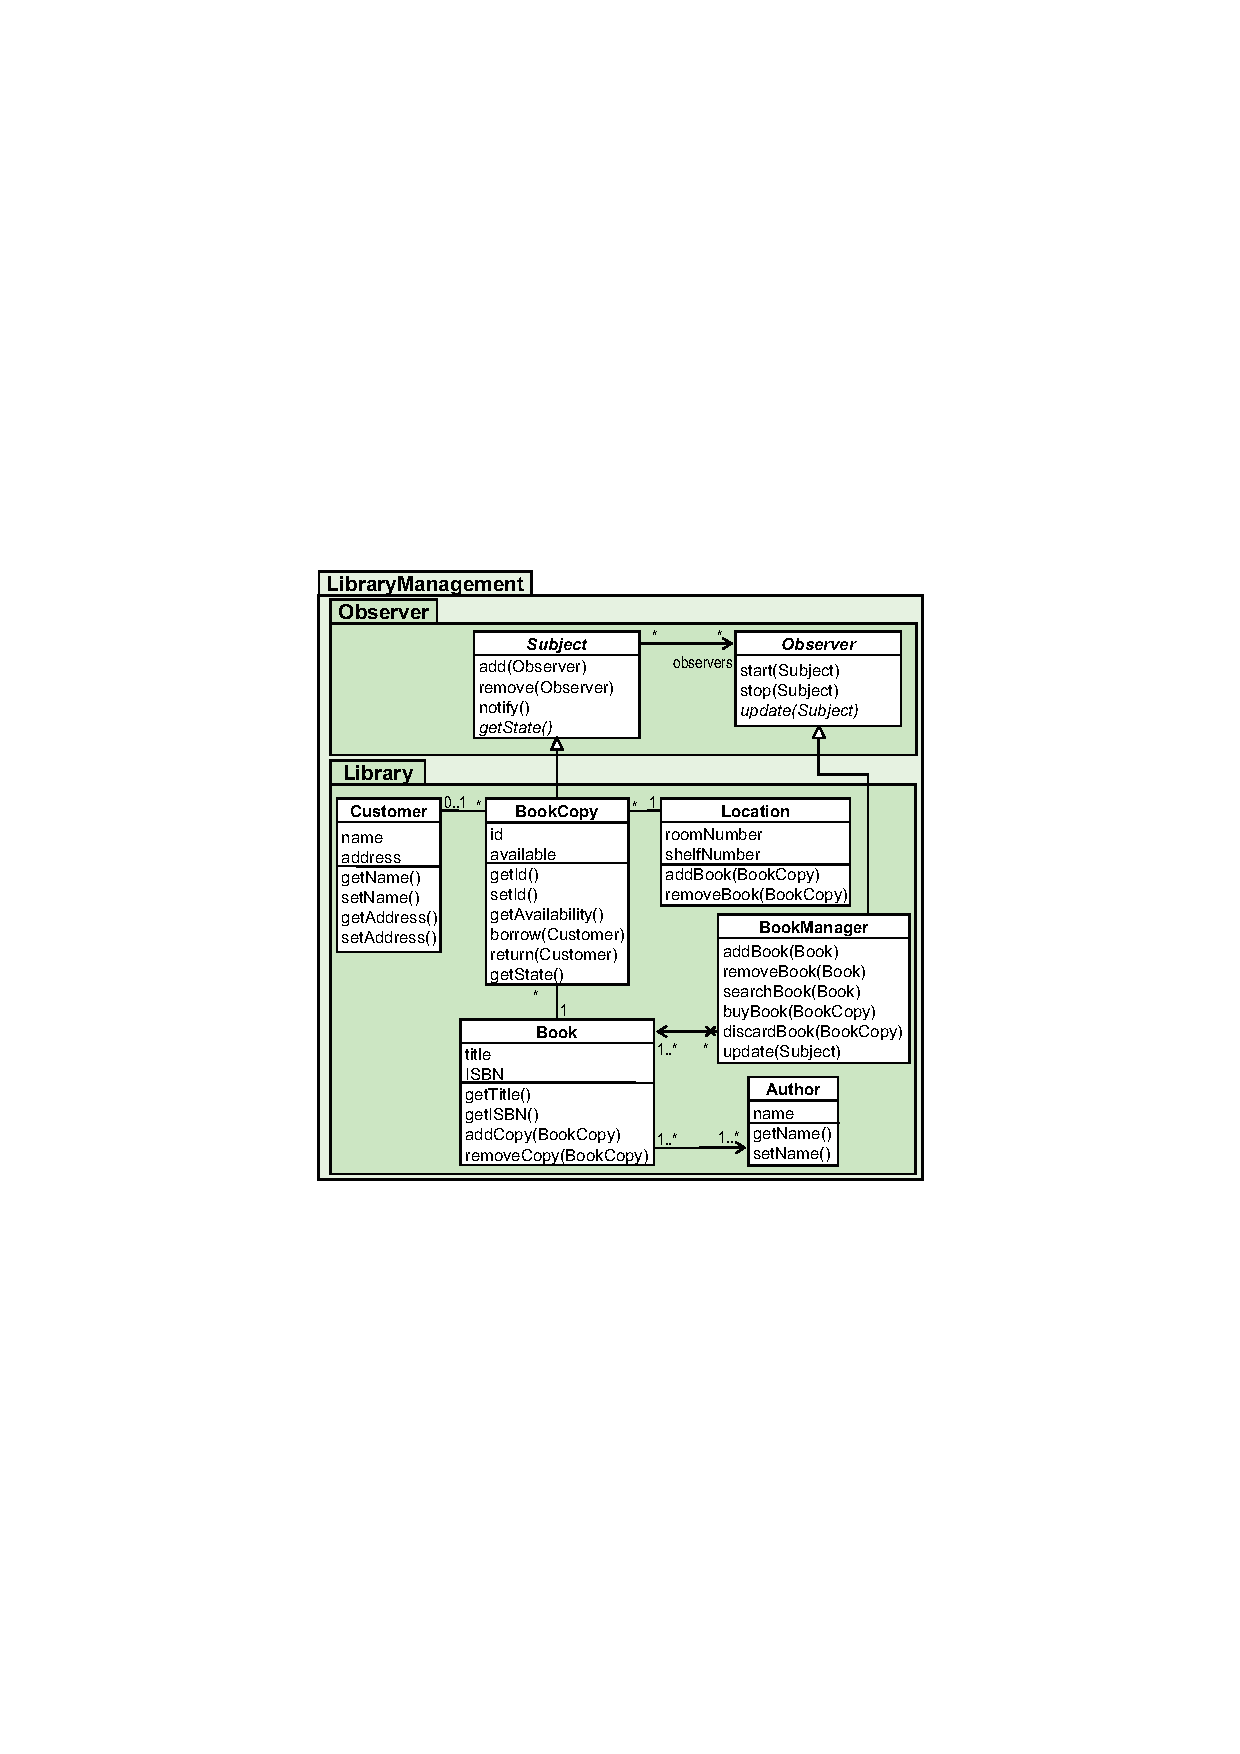
\includegraphics[width=0.7\textwidth]{figures/figure1}
	\caption{Sample figure}
	\label{fig:samplefigure_pdf}
\end{figure}


\section{Fonts}

When introducing important terms for the first time use \emph{emphasize}. For a consistent look and feel of proper names like {\cd} and {\uml{Observer}} pattern you may define macros in the main document \texttt{thesis.tex}.

\section{Code}

For short code fragments use the \textit{verbatim} environment.

\begin{verbatim}
//Start Program
System.out.println("Hello World!");
//End Program
\end{verbatim}

A much better alternative is the \textit{algorithm} environment (cf. Algorithm~\ref{alg:samplealgorithm}). This environment offers special formatting features for loops, operations and comments.

\begin{algorithm}[t]
\SetKwData{Left}{left}
\SetKwData{This}{this}
\SetKwData{Up}{up}
\SetKwFunction{Union}{Union}
\SetKwFunction{FindCompress}{FindCompress}
\SetKwInOut{Input}{input}
\SetKwInOut{Output}{output}

\Input{A bitmap $Im$ of size $w\times l$}
\Output{A partition of the bitmap}

\BlankLine

\emph{special treatment of the first line}\;
\For{$i\leftarrow 2$ \KwTo $l$}{
\emph{special treatment of the first element of line $i$}\;
\For{$j\leftarrow 2$ \KwTo $w$}{\label{forins}
\Left$\leftarrow$ \FindCompress{$Im[i,j-1]$}\;
\Up$\leftarrow$ \FindCompress{$Im[i-1,]$}\;
\This$\leftarrow$ \FindCompress{$Im[i,j]$}\;
\If(\tcp*[r]{O(\Left,\This)==1}){\Left compatible with \This}{\label{lt}
\lIf{\Left $<$ \This}{\Union{\Left,\This}}\;
\lElse{\Union{\This,\Left}\;}
}
\If(\tcp*[r]{O(\Up,\This)==1}){\Up compatible with \This}{\label{ut}
\lIf{\Up $<$ \This}{\Union{\Up,\This}}\;
\tcp{\This is put under \Up to keep tree as flat as possible}\label{cmt}
\lElse{\Union{\This,\Up}}\tcp*[r]{\This linked to \Up}\label{lelse}
}
}
\lForEach{element $e$ of the line $i$}{\FindCompress{p}}
}
\caption{Sample algorithm}\label{alg:samplealgorithm}
\end{algorithm}



%%%%%%%%%%%%%%%%%%%%%%%%%%%%%%%%%%%%%%%%%
%\chapter{Bibliographic Issues}
%\label{ch:bibliographic}
%%%%%%%%%%%%%%%%%%%%%%%%%%%%%%%%%%%%%%%%%

%\section{Literature Search}

Information on online libraries and literature search, e.g., interesting magazines, journals, conferences, and organizations may be found at \url{http://www.big.tuwien.ac.at/teaching/info.html}.

\section{BibTeX}

BibTeX should be used for referencing.

Blabla article1 \cite{hetzl2012towards}, laber laber article2 \cite{hetzl2014article}.

%%%%%%%%%%%%%%%%%%%%%%%%%%%%%%%%%%%%%%%%%
%%% BACKMATTER %%%%%%%%%%%%%%%%%%%%%%%%%%
%%%%%%%%%%%%%%%%%%%%%%%%%%%%%%%%%%%%%%%%%

\appendix

\bibliographystyle{plain}
\bibliography{references1}

\end{document}
